\documentclass[a4paper]{scrartcl}

\usepackage[
	fancytheorems,
	fancyproofs,
	noindent
]{adam}

\usepackage{tikz}
\usetikzlibrary{decorations.markings}

\newcommand{\id}{\operatorname{id}}
\newcommand{\genby}[1]{\langle #1 \rangle}
\newcommand{\Cinf}{\C_\infty}
\newcommand{\disc}{\mathbb{D}}
\newcommand{\Hp}{\mathbb{H}}
\newcommand{\Cs}{\C^*}
\newcommand{\mult}{\operatorname{mult}}
\newcommand{\vaL}{\operatorname{val}}
\newcommand{\Deck}{\operatorname{Deck}}
\newcommand{\res}{\operatorname{res}}

\title{Riemann Surfaces}
\author{Adam Kelly (\texttt{ak2316@cam.ac.uk})}
\date{\today}

\allowdisplaybreaks

\begin{document}

\maketitle

Complex analysis is full of functions that refuse to be functions. The logarithm is the
obvious offender: $\exp$ is surjective onto $\C^*$ but wildly non-injective, so `the'
logarithm of $z$ is only defined once we have made a choice, and no choice can be made
consistently on all of $\C^*$. The same is true of $\sqrt{z}$, of $\sqrt{z^3 - z}$, and
of the inverse of essentially any interesting holomorphic map. The traditional response
is to slit the plane along a branch cut and work on what is left, but this is a
confession of defeat: the cut is an artefact of our bookkeeping, not of the function,
and the whole interest of $\log$ lies precisely in what happens when you walk around the
origin and come back changed.

Riemann's idea was to stop mutilating the domain and start enlarging it. If $\log$ wants
to take infinitely many values at each point of $\C^*$, then give it a domain with
infinitely many points lying over each point of $\C^*$ -- an infinite spiral ramp -- on
which it becomes an honest single-valued holomorphic function. The price is that this new
domain is no longer an open subset of $\C$; it is a space which merely \emph{looks like}
$\C$ near each of its points. That is a Riemann surface, and once we allow ourselves such
objects a great deal falls into place. Multi-valued functions become genuine functions,
branch cuts become invisible, and -- most strikingly -- the analysis starts to control the
topology. We will prove the Riemann--Hurwitz formula, which says that a holomorphic map
between compact surfaces forces a numerical relation between their genera and its
branching, and we will use it to compute the genus of a surface from nothing more than
the equation that cuts it out.

This article constitutes my notes for the `Riemann Surfaces' course, held in Michaelmas
2022 at Cambridge. These notes are \emph{not a transcription of the lectures}, and differ
significantly in quite a few areas. Still, all lectured material should be covered.

\tableofcontents

\section{Holomorphic Functions Revisited}

We begin by recalling, mostly without proof, what IB Complex Analysis gives us. Nothing
in this section is new, but the results here are the local engine driving everything
later on: every theorem we prove about Riemann surfaces will ultimately be a theorem
about holomorphic functions on discs, transported by charts.

\subsection{Analytic Functions and their Zeros}

\begin{definition}[Domain]
	A \vocab{domain} is a non-empty open connected subset $D \subseteq \C$.
\end{definition}

Open discs $D(a, r) = \{z : |z - a| < r\}$, punctured discs $D(a,r) \setminus \{a\}$,
annuli, half-planes and slit planes are all domains, and these are essentially the only
ones we will ever need to write down explicitly.

\begin{definition}[Holomorphic Function]
	Let $D \subseteq \C$ be a domain. A function $f: D \to \C$ is \vocab{holomorphic}
	(or \vocab{analytic}) if it is complex differentiable at every point of $D$.
\end{definition}

The great theorem of IB Complex Analysis is that this weak-looking hypothesis is
enormously strong: a holomorphic function is automatically infinitely differentiable,
and is represented by its Taylor series on any disc contained in its domain. In
particular `complex differentiable everywhere' and `locally the sum of a convergent
power series' mean the same thing, and we shall use the two descriptions
interchangeably.\footnote{This is why the words `holomorphic' and `analytic' are used
as synonyms throughout. In the real setting they are very much not synonyms.}

The first consequence we need concerns zeros. A holomorphic function cannot vanish on a
set with an accumulation point without vanishing identically -- its zeros are isolated.

\begin{proposition}[Isolated Zeros]\label{prop:isolatedzeros}
	Let $f$ be holomorphic on a domain $D$ and suppose $f(z_0) = 0$. Then either $f$ is
	identically zero on $D$, or there is a punctured disc about $z_0$ on which $f$ does
	not vanish.
\end{proposition}

\begin{proof}
	Write $f(z) = \sum_{n \geq 0} a_n (z - z_0)^n$ on some disc $U = D(z_0, r) \subseteq D$.
	If every $a_n$ vanishes then $f \equiv 0$ on $U$, and a connectedness argument (the set
	where all derivatives of $f$ vanish is open and closed in $D$) gives $f \equiv 0$ on all
	of $D$.

	Otherwise let $m \geq 0$ be minimal with $a_m \neq 0$, so that on $U$ we may write
	$$
	f(z) = (z - z_0)^m g(z), \qquad g(z) = \sum_{n \geq 0} a_{m + n}(z - z_0)^n.
	$$
	The series for $g$ converges on $U$, so $g$ is holomorphic there, and $g(z_0) = a_m \neq 0$.
	By continuity $g$ is non-vanishing on some disc $D(z_0, \delta)$, and therefore $f$ is
	non-vanishing on $D(z_0,\delta) \setminus \{z_0\}$.
\end{proof}

The integer $m$ appearing in the proof is the \vocab{order} of the zero of $f$ at $z_0$,
and it is worth noticing now -- because the observation is the whole of Section
\ref{sec:branching} in disguise -- that near such a point $f$ looks like $z \mapsto z^m$
multiplied by a non-vanishing function.

\begin{corollary}[Identity Theorem]\label{cor:identity}
	Let $f, g$ be holomorphic on a domain $D$. If the set $\{z \in D : f(z) = g(z)\}$ has
	an accumulation point in $D$, then $f = g$ on $D$.
\end{corollary}

\begin{proof}
	Apply Proposition \ref{prop:isolatedzeros} to $f - g$: the agreement set is not
	discrete, so $f - g$ cannot have isolated zeros, and hence vanishes identically.
\end{proof}

This is the single most important fact in the course. It says a holomorphic function has
no local freedom whatsoever: its germ at one point determines it everywhere on a
connected domain. All of analytic continuation is an attempt to exploit this rigidity,
and all of the trouble with analytic continuation comes from the word `connected'.

\subsection{Singularities and Meromorphic Functions}

\begin{definition}[Isolated Singularity]
	A function $f$ holomorphic on a punctured disc $D(z_0, r) \setminus \{z_0\}$ is said
	to have an \vocab{isolated singularity} at $z_0$.
\end{definition}

On such a punctured disc $f$ has a Laurent expansion
$$
f(z) = \sum_{n = -\infty}^{\infty} a_n (z - z_0)^n,
$$
converging locally uniformly, and the singularity is classified by the tail of negative
coefficients.

\begin{definition}[Types of Singularity]
	With notation as above, we say $z_0$ is
	\begin{enumerate}[label=(\roman*)]
		\item a \vocab{removable singularity} if $a_n = 0$ for all $n < 0$;
		\item a \vocab{pole of order} $m > 0$ if $a_{-m} \neq 0$ and $a_n = 0$ for all $n < -m$;
		\item an \vocab{essential singularity} otherwise.
	\end{enumerate}
	A pole of order $1$ is called \vocab{simple}.
\end{definition}

\begin{theorem}[Riemann Removable Singularity Theorem]\label{thm:removable}
	If $f$ is holomorphic and bounded on a punctured disc about $z_0$, then $z_0$ is a
	removable singularity, and $f$ extends holomorphically over $z_0$.
\end{theorem}

\begin{theorem}[Casorati--Weierstrass]\label{thm:casorati}
	The point $z_0$ is an essential singularity of $f$ if and only if $f(U)$ is dense in
	$\C$ for every punctured neighbourhood $U$ of $z_0$.
\end{theorem}

Both were proved in IB Complex Analysis and we take them as given. The trichotomy is
worth restating in the form we shall actually use: as $z \to z_0$, either $f(z)$ tends to
a limit in $\C$ (removable), or $|f(z)| \to \infty$ (pole), or $f$ oscillates so violently
that it comes arbitrarily close to every complex number (essential). Poles are therefore
not really singularities at all if we are willing to let $\infty$ count as a value, and
that willingness is exactly what the Riemann sphere will formalise.

\begin{definition}[Meromorphic Function]
	Let $D$ be a domain and $A \subseteq D$ a discrete closed subset. A holomorphic
	function $f : D \setminus A \to \C$ with a pole at each point of $A$ is called
	\vocab{meromorphic} on $D$.
\end{definition}

\begin{example}
	The function
	$$
	f(z) = \frac{1}{e^{1/z} - 1}
	$$
	is meromorphic on the upper half-plane, with simple poles at the points
	$1/(2\pi i n)$ for $n \in \N$. Note what happens if we try to regard $f$ as meromorphic
	on all of $\C$: the poles accumulate at $0$, so the set of poles is no longer discrete
	as a subset of $\C$, and indeed $0$ is an essential singularity of $f$. The condition
	that $A$ be discrete \emph{and closed in $D$} is doing real work.
\end{example}

\subsection{The Open Mapping Theorem and the Maximum Modulus Principle}

The last two facts we shall want are global in flavour.

\begin{theorem}[Open Mapping Theorem]\label{thm:omtplane}
	A non-constant holomorphic function on a domain $D \subseteq \C$ is an open map.
\end{theorem}

\begin{theorem}[Maximum Modulus Principle]\label{thm:maxmodplane}
	Let $f$ be holomorphic on a domain $D$. If $|f|$ attains a local maximum at some
	point of $D$, then $f$ is constant.
\end{theorem}

The second follows immediately from the first: if $f(D)$ is open then no point of $f(D)$
can be a point of maximum modulus of $f(D)$, since every neighbourhood of a point $w$
contains points of larger modulus.

Finally we record the local statement that will become the definition of multiplicity.

\begin{theorem}[Inverse Function Theorem]\label{thm:ift}
	Let $f$ be holomorphic near $z_0$ with $f'(z_0) \neq 0$. Then there are open
	neighbourhoods $U \ni z_0$ and $V \ni f(z_0)$ such that $f|_U : U \to V$ is a
	biholomorphism, i.e.\ a holomorphic bijection with holomorphic inverse.
\end{theorem}

\section{Analytic Continuation}

We now come to the problem that motivates the whole course. The identity theorem says
that a holomorphic function on a domain is determined by its restriction to any small
disc. Turning this around: given a holomorphic function on a small disc, can we recover
`the' function it came from, on some larger domain? And if we can do it in more than one
way, how do the answers differ?

\subsection{Function Elements and Direct Continuation}

\begin{definition}[Function Element]
	Let $D \subseteq \C$ be a domain. A \vocab{function element} on $D$ is a pair
	$(f, U)$ where $U \subseteq D$ is a subdomain and $f : U \to \C$ is holomorphic.
\end{definition}

\begin{definition}[Direct Analytic Continuation]
	Two function elements $(f, U)$ and $(g, V)$ on $D$ are \vocab{direct analytic
	continuations} of one another, written $(f, U) \sim (g, V)$, if $U \cap V \neq \emptyset$
	and $f = g$ on $U \cap V$.
\end{definition}

\begin{center}
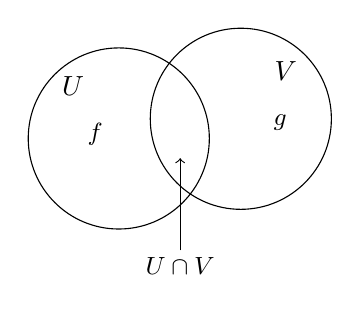
\begin{tikzpicture}[scale=1]
	\draw[thin] (0,0) circle (1.15);
	\draw[thin] (1.55,0.25) circle (1.15);
	\node at (-0.58,0.66) {$U$};
	\node at (2.12,0.86) {$V$};
	\node at (0.78,-1.62) {\small $U \cap V$};
	\draw[->,thin] (0.78,-1.42) -- (0.78,-0.25);
	\node at (-0.3,0.05) {\small $f$};
	\node at (2.05,0.2) {\small $g$};
\end{tikzpicture}
\end{center}

By the identity theorem, if $U \cap V$ is connected then $g$ is completely determined by
$f$ (and by the choice of $V$): there is at most one holomorphic $g$ on $V$ agreeing with
$f$ on $U \cap V$. If $U \cap V$ is disconnected the definition still makes sense, but we
should be careful, since agreeing on one component is then weaker than agreeing on all of
them. We will normally arrange for our sets to be discs, so that intersections are convex
and this issue evaporates.

The relation $\sim$ is reflexive and symmetric but emphatically \emph{not} transitive --
that failure is the entire subject. So we take its transitive closure.

\begin{definition}[Analytic Continuation]
	We write $(f, U) \approx (g, V)$ if there is a finite chain of function elements
	$$
	(f, U) = (f_0, U_0) \sim (f_1, U_1) \sim \cdots \sim (f_n, U_n) = (g, V)
	$$
	on $D$. We then say $(g,V)$ is an \vocab{analytic continuation} of $(f,U)$.
\end{definition}

Now $\approx$ \emph{is} an equivalence relation, being the transitive closure of a
reflexive symmetric relation.

\begin{definition}[Complete Analytic Function]
	An equivalence class $\mathcal{F}$ of function elements on $D$ under $\approx$ is
	called a \vocab{complete analytic function} on $D$.
\end{definition}

The name is a little grandiose for what is, at this stage, just a set of pairs. But the
point of view is the right one: a `multi-valued function' is not a function with several
values, it is a \emph{collection of ordinary functions, glued along their overlaps}. Our
job over the next few sections is to make the gluing literal.

\subsection{The Complex Logarithm}\label{subsec:logelements}

Let us do the fundamental example completely explicitly. Write $\Cs = \C \setminus \{0\}$,
and recall that $\exp : \C \to \Cs$ is surjective with $\exp(z) = \exp(w)$ if and only if
$z - w \in 2\pi i \Z$. We want to invert it.

For an interval $(\alpha, \beta) \subseteq \R$ with $\beta - \alpha \leq 2\pi$, set
$$
U_{(\alpha, \beta)} = \{ r e^{i\theta} : r > 0, \ \alpha < \theta < \beta\},
$$
an open sector, and define $f_{(\alpha,\beta)} : U_{(\alpha,\beta)} \to \C$ by
$$
f_{(\alpha,\beta)}(re^{i\theta}) = \log r + i \theta, \qquad \theta \in (\alpha,\beta).
$$
This is well defined precisely because the angle $\theta$ of a point of
$U_{(\alpha,\beta)}$ is unique in the range $(\alpha,\beta)$, and it is holomorphic since
it is a local inverse of $\exp$, which has non-vanishing derivative. So
$$
F_{(\alpha,\beta)} = (f_{(\alpha,\beta)}, U_{(\alpha,\beta)})
$$
is a function element on $\Cs$, and $\exp \circ f_{(\alpha,\beta)} = \id$.

To keep the bookkeeping finite, restrict attention to quarter-turn sectors: for
$n \in \Z$ put
$$
I(n) = \left( \frac{(n-1)\pi}{2}, \frac{(n+1)\pi}{2} \right),
$$
an interval of length $\pi$ centred on $n\pi/2$, and abbreviate $U_n = U_{I(n)}$,
$f_n = f_{I(n)}$, $F_n = F_{I(n)}$. Thus $U_0$ is the right half-plane, $U_1$ the upper
half-plane, and so on; $U_n$ depends only on $n$ modulo $4$, but $f_n$ does not.

\begin{proposition}\label{prop:logelements}
	$F_m \sim F_n$ if and only if $|m - n| \leq 1$.
\end{proposition}

\begin{proof}
	First suppose $|m-n| \leq 1$. If $m = n$ there is nothing to do, so take $n = m+1$.
	Then $U_m \cap U_{m+1}$ is the open sector of angles in $(m\pi/2, (m+1)\pi/2)$, which
	is non-empty, and for $z = re^{i\theta}$ in it we may take $\theta$ in that common
	range, whence $f_m(z) = \log r + i\theta = f_{m+1}(z)$. So $F_m \sim F_{m+1}$.

	Conversely suppose $|m - n| \geq 2$. If $|m - n| \geq 4$ then $I(m)$ and $I(n)$ are
	disjoint modulo nothing at all -- more precisely the sectors $U_m, U_n$ may still
	meet, but any $z$ in the intersection has $f_m(z) - f_n(z) \in 2\pi i \Z \setminus \{0\}$,
	since the two determinations of the argument differ by a non-zero multiple of $2\pi$.
	If $|m-n| = 2$ then $U_m$ and $U_n$ are opposite half-planes meeting in two opposite
	quadrants, and $|m - n| = 3$ gives an intersection which is a single quadrant; in every
	case a point of the intersection has $f_m(z) \neq f_n(z)$, because the arguments used
	differ by a non-zero multiple of $2\pi$. Hence $F_m \not\sim F_n$.
\end{proof}

\begin{corollary}\label{cor:logconnected}
	$F_m \approx F_n$ for all $m, n \in \Z$.
\end{corollary}

\begin{proof}
	Chain along $F_m \sim F_{m\pm 1} \sim \cdots \sim F_n$.
\end{proof}

So all the $F_n$ lie in a single complete analytic function on $\Cs$, which we may
reasonably call \emph{the} complex logarithm. Notice what has happened: $U_0 = U_4$ as
subsets of $\C$, but
$$
f_0(1) = 0, \qquad f_4(1) = 2\pi i.
$$
Continuing once round the origin has changed the function. Analytic continuation is
therefore \emph{not} path-independent, and the complete analytic function $\log$ is
genuinely bigger than any one of its elements.

\begin{center}
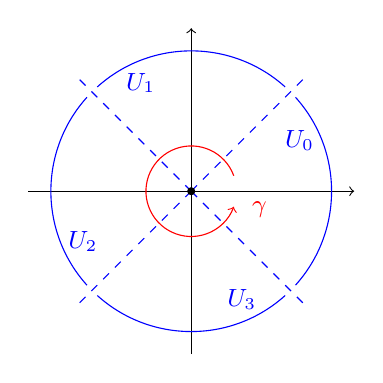
\begin{tikzpicture}[scale=1.15]
	\draw[thin,->] (-1.8,0) -- (1.8,0);
	\draw[thin,->] (0,-1.8) -- (0,1.8);
	\foreach \st/\en/\lab/\pos in {-42/42/{U_0}/25, 48/132/{U_1}/115, 138/222/{U_2}/205, 228/312/{U_3}/295} {
		\draw[thin, color=blue] (\st:1.55) arc (\st:\en:1.55);
		\node[color=blue] at (\pos:1.32) {\small $\lab$};
	}
	\foreach \a in {45,135,225,315} { \draw[thin, dashed, color=blue] (0,0) -- (\a:1.78); }
	\fill (0,0) circle (0.045);
	\draw[->, thin, color=red] (20:0.5) arc (20:340:0.5);
	\node[color=red] at (-15:0.78) {\small $\gamma$};
\end{tikzpicture}
\end{center}

The four half-planes $U_0, \dots, U_3$ cover $\Cs$, and each overlaps the next in a
quadrant. Continuing $f_0$ around the loop $\gamma$ takes us through $F_1, F_2, F_3$ and
back to $U_0$, but with $f_4 = f_0 + 2\pi i$.

\subsection{Complex Roots}

Exactly the same analysis handles $k$-th roots. Let $p_k : \Cs \to \Cs$ be $z \mapsto z^k$
for $k \geq 2$, and define, on the same sectors $U_n$ as above,
$$
g_n(z) = \exp\left(\tfrac{1}{k} f_n(z)\right), \qquad G_n = (g_n, U_n).
$$
Then $g_n(z)^k = \exp(f_n(z)) = z$, so each $g_n$ is a holomorphic branch of the $k$-th
root on $U_n$.

Since $f_{n + 4}= f_n + 2\pi i$ we get $g_{n+4} = e^{2\pi i /k} g_n$, and more generally
$g_n$ depends only on $n$ modulo $4k$. Repeating the case analysis of Proposition
\ref{prop:logelements} shows that $G_m \sim G_n$ if and only if $m \equiv n$ or
$m \equiv n \pm 1$ modulo $4k$, and hence all the $G_n$ lie in a single complete analytic
function. This time, though, going round the origin \emph{four} times returns us to
$e^{2\pi i / k}g_0$, and it takes $k$ circuits to get back to where we started. The
multi-valuedness of $\sqrt[k]{\cdot}$ is finite, of order $k$, where that of $\log$ was
infinite.

\subsection{Natural Boundaries}

Before building surfaces, we pause on an obstruction: sometimes a function element admits
no continuation at all past the boundary of its natural domain.

Write $\disc = D(0,1)$ and $\mathbb{T} = \partial \disc$. Let $f(z) = \sum_{n \geq 0} a_n z^n$
be a power series with radius of convergence exactly $1$, so that $(f, \disc)$ is a
function element.

\begin{definition}[Regular and Singular Points]
	A point $z_0 \in \mathbb{T}$ is \vocab{regular} for $f$ if there is an open
	neighbourhood $U$ of $z_0$ and a function element $(g, U)$ with $g = f$ on
	$U \cap \disc$. Otherwise $z_0$ is \vocab{singular} for $f$.
\end{definition}

The set of regular points is visibly open in $\mathbb{T}$, so the singular points form a
closed set. It is tempting to think that $z_0$ is regular exactly when the power series
converges at $z_0$, and this is false in both directions.

\begin{example}
	Take $f(z) = 1/(1-z) = \sum_{n \geq 0} z^n$. The only singular point is $z = 1$, so
	$z = -1$ is regular; but the power series $\sum (-1)^n$ does not converge at $-1$.
	Convergence is not necessary for regularity.
\end{example}

\begin{example}
	Take $g(z) = \sum_{n \geq 2} \frac{z^n}{n(n-1)}$. This converges absolutely at
	$z = 1$. But $g''(z) = \sum_{n\geq 2} z^{n-2} = 1/(1-z)$, which is singular at $1$; so
	$g$ cannot be continued past $1$ either, and $1$ is singular for $g$. Convergence is
	not sufficient for regularity.
\end{example}

\begin{proposition}
	If $f(z) = \sum_{n \geq 0}a_n z^n$ has radius of convergence exactly $1$, then some
	point of $\mathbb{T}$ is singular for $f$.
\end{proposition}

\begin{proof}
	Suppose not. Then every $z_0 \in \mathbb{T}$ has a disc $D(z_0, \varepsilon_{z_0})$
	carrying a continuation of $f$. By compactness finitely many such discs cover
	$\mathbb{T}$; by the identity theorem (the intersections being convex, hence connected)
	these continuations agree with each other and with $f$ on overlaps, and so patch
	together with $f$ to give a holomorphic function on an open set containing
	$\overline{\disc}$. That set contains $D(0, 1 + \delta)$ for some $\delta > 0$, again
	by compactness, and so the Taylor series of $f$ at $0$ would have radius of convergence
	at least $1 + \delta$, a contradiction.
\end{proof}

\begin{definition}[Natural Boundary]
	If every point of $\mathbb{T}$ is singular for $f$, we call $\mathbb{T}$ the
	\vocab{natural boundary} of $f$.
\end{definition}

\begin{example}[A Lacunary Series]
	Let $f(z) = \sum_{n \geq 0} z^{n!}$, which has radius of convergence $1$. We claim
	$\mathbb{T}$ is its natural boundary.

	Since the singular set is closed, it suffices to show that the roots of unity are all
	singular, as these are dense in $\mathbb{T}$. So let $\omega = e^{2\pi i p /q}$ with
	$p, q \in \Z$, $q \geq 1$. For $n \geq q$ we have $q \mid n!$ and so
	$\omega^{n!} = 1$. Hence for $r \in (0,1)$,
	$$
	f(r\omega) = \sum_{n = 0}^{q-1} r^{n!}\omega^{n!} + \sum_{n \geq q} r^{n!}.
	$$
	The first sum is a finite sum of terms of modulus at most $1$, hence bounded by $q$.
	For the second, given any $M > 0$ we have
	$$
	\sum_{n \geq q} r^{n!} \geq \sum_{n = q}^{q + M} r^{n!} \longrightarrow M + 1
	$$
	as $r \to 1^-$, so $\sum_{n\geq q} r^{n!} > M$ for $r$ close enough to $1$. Therefore
	$f(r\omega) \to \infty$ as $r \to 1^-$. A function element $(g,U)$ agreeing with $f$
	near $\omega$ would be bounded near $\omega$, so no such element exists and $\omega$
	is singular.
\end{example}

So continuation can fail entirely. When it does not fail, we would like to understand how
the answer depends on the route taken -- which requires us to say what a route is.

\subsection{Continuation Along a Path}

\begin{definition}[Continuation Along a Path]\label{def:contpath}
	Let $\gamma : [0,1] \to D$ be a path and let $(f, U), (g, V)$ be function elements on
	$D$ with $\gamma(0) \in U$ and $\gamma(1) \in V$. We write $(f, U) \approx_\gamma (g,V)$
	if there is a dissection $0 = t_0 < t_1 < \cdots < t_n = 1$ and function elements
	$$
	(f, U) = (f_1, U_1), \ (f_2, U_2), \ \dots, \ (f_n, U_n) = (g, V)
	$$
	with $(f_i, U_i) \sim (f_{i+1}, U_{i+1})$ for each $i$, and
	$\gamma([t_{i-1}, t_i]) \subseteq U_i$ for each $i$. We then say $(f,U)$ can be
	\vocab{continued along $\gamma$}, with result $(g,V)$.
\end{definition}

\begin{center}
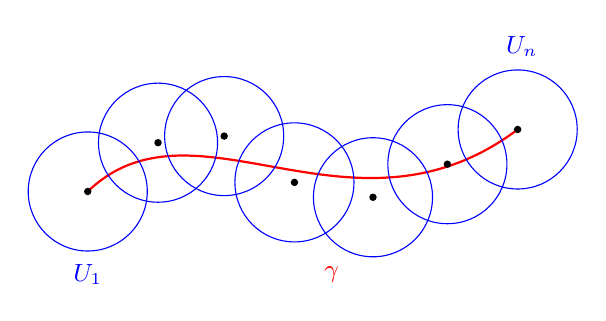
\begin{tikzpicture}[scale=1.05]
	\draw[thick, color=red] (-2.6,-0.35) .. controls (-1.3,0.9) and (0.6,-1.1) .. (2.6,0.4);
	\foreach \x/\y in {-2.6/-0.35, -1.75/0.24, -0.95/0.32, -0.1/-0.24, 0.85/-0.42, 1.75/-0.02, 2.6/0.4} {
		\draw[thin, color=blue] (\x,\y) circle (0.72);
	}
	\foreach \x/\y in {-2.6/-0.35, -1.75/0.24, -0.95/0.32, -0.1/-0.24, 0.85/-0.42, 1.75/-0.02, 2.6/0.4} {
		\fill (\x,\y) circle (0.045);
	}
	\node[color=blue] at (-2.6,-1.35) {\small $U_1$};
	\node[color=blue] at (2.65,1.4) {\small $U_n$};
	\node[color=red] at (0.35,-1.35) {\small $\gamma$};
\end{tikzpicture}
\end{center}

The picture is a chain of discs strung along $\gamma$, each carrying a holomorphic
function agreeing with its neighbours. Definition \ref{def:contpath} is a little
unwieldy, and we will replace it in Section \ref{sec:germs} by something much cleaner:
continuation along $\gamma$ will simply be \emph{lifting $\gamma$ to the space of germs}.
Once we have said that, the key uniqueness statement -- the monodromy theorem, that the
result of continuing along $\gamma$ depends only on the homotopy class of $\gamma$ --
becomes a special case of the homotopy lifting property from IB/II Algebraic Topology.

\section{The Surfaces of $\log$ and $\sqrt[k]{z}$}\label{sec:logsurface}

Before setting up the general theory, let us build the two surfaces the theory is meant
to explain. This is worth doing by hand: everything we do abstractly later is modelled
on these two constructions.

\subsection{Gluing the Sectors}

Recall from Section \ref{subsec:logelements} the function elements $F_n = (f_n, U_n)$
for $\log$. The trouble was that $U_0$ and $U_4$ are the same subset of $\C$ but carry
different functions. So let us refuse to identify them. Define
$$
R = \left( \coprod_{n \in \Z} U_n \right) \Big/ \sim,
$$
where a point $z_1$ in the copy $U_m$ is identified with a point $z_2$ in the copy $U_n$
if and only if
$$
z_1 = z_2 \text{ as elements of } \C \quad \text{and} \quad f_m(z_1) = f_n(z_2),
$$
and give $R$ the quotient topology. In words: we lay out infinitely many copies of the
sectors, and glue copy $m$ to copy $n$ exactly where the two branches of $\log$ agree. By
Proposition \ref{prop:logelements} this happens exactly when $|m - n| \leq 1$, so each
sector is glued to its two neighbours along a quadrant, and the result spirals.

The picture to have in mind is an infinite multi-storey car park: a helical ramp winding
endlessly up and down over the punctured plane, with no floor ever meeting another except
its immediate neighbours.

\begin{center}
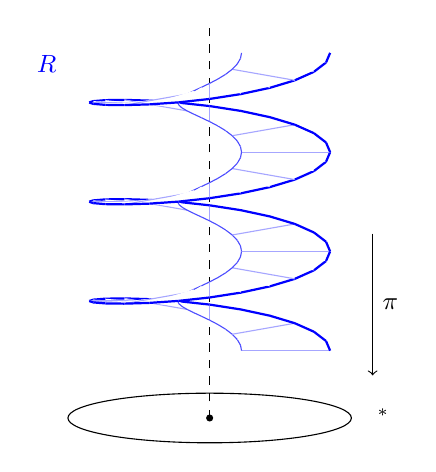
\begin{tikzpicture}[scale=0.9]
	% base punctured plane
	\draw[thin] (0,-2.9) ellipse (2.0 and 0.35);
	\fill (0,-2.9) circle (0.05);
	\node at (2.45,-2.9) {\small $\Cs$};
	% axis through the puncture
	\draw[thin, dashed] (0,-2.9) -- (0,2.6);
	% helicoid: three turns, drawn as white-filled strips in order of increasing angle
	% so that the near part of the ramp correctly overdraws whatever lies behind it
	\foreach \t in {0,15,...,1065} {
		\pgfmathsetmacro\tb{\t+15}
		\pgfmathsetmacro\ya{0.30*sin(\t) + \t*0.003889 - 1.95}
		\pgfmathsetmacro\yb{0.30*sin(\tb) + \tb*0.003889 - 1.95}
		\pgfmathsetmacro\yc{0.08*sin(\tb) + \tb*0.003889 - 1.95}
		\pgfmathsetmacro\yd{0.08*sin(\t) + \t*0.003889 - 1.95}
		\pgfmathtruncatemacro\sp{mod(\t,45)}
		\fill[white] ({1.7*cos(\t)},\ya) -- ({1.7*cos(\tb)},\yb) --
			({0.45*cos(\tb)},\yc) -- ({0.45*cos(\t)},\yd) -- cycle;
		\ifnum\sp=0
			\draw[color=blue!35, thin] ({1.7*cos(\t)},\ya) -- ({0.45*cos(\t)},\yd);
		\fi
		\draw[color=blue, thick] ({1.7*cos(\t)},\ya) -- ({1.7*cos(\tb)},\yb);
		\draw[color=blue!70, thin] ({0.45*cos(\t)},\yd) -- ({0.45*cos(\tb)},\yc);
	}
	\draw[->, thin] (2.3,-0.3) -- (2.3,-2.3);
	\node at (2.55,-1.3) {\small $\pi$};
	\node[color=blue] at (-2.3,2.1) {\small $R$};
\end{tikzpicture}
\end{center}

Two maps come along for free. First, the branches assemble into a single global function:
define $f : R \to \C$ by $f([z]) = f_n(z)$ for $z \in U_n$. This is well defined precisely
because we built the equivalence relation to make it so. Second, the inclusions
$U_n \hookrightarrow \Cs$ assemble into $\pi : R \to \Cs$, $\pi([z]) = z$, which is well
defined because equivalent points are equal in $\C$. These satisfy
$$
\exp \circ f = \pi,
$$
which says exactly that $f$ deserves the name `logarithm': applying $\exp$ to $f$ recovers
the point of $\Cs$ underneath.

\begin{proposition}
	$R$ is path-connected and Hausdorff.
\end{proposition}

\begin{proof}
	Path-connectedness: each $U_n$ is connected, and $U_n$ meets $U_{n+1}$ in $R$ (as
	$F_n \sim F_{n+1}$), so the images of the $U_n$ in $R$ form a chain of overlapping
	connected sets covering $R$.

	For Hausdorffness, consider $\Phi : R \to \C^2$ given by
	$$
	\Phi([z]) = (\pi([z]), f([z])).
	$$
	This is continuous, and it is injective: if $\Phi([z_1]) = \Phi([z_2])$ then $z_1 = z_2$
	in $\C$ and the two branch values agree, which is precisely the condition defining
	$\sim$. A continuous injection into a Hausdorff space separates points, so $R$ is
	Hausdorff.
\end{proof}

\begin{remark}
	In fact $\Phi$ identifies $R$ with the graph
	$$
	\{(w, z) \in \C^2 : w = \exp z\},
	$$
	and under this identification $\pi$ and $f$ are the two coordinate projections. So the
	Riemann surface of $\log$ is nothing more exotic than the graph of $\exp$ with the
	roles of the axes swapped. This is a useful sanity check, and a preview: in general,
	the Riemann surface of an algebraic function will be (a compactification of) the graph
	of the equation defining it.
\end{remark}

\subsection{The Surface of the $k$-th Root}

The same construction with the elements $G_n = (g_n, U_n)$ produces a space $R_k$. Since
$g_n$ depends only on $n$ modulo $4k$, this time only $4k$ copies of the sectors are
involved and the spiral closes up after $k$ turns. We again get $g : R_k \to \Cs$ and
$\pi : R_k \to \Cs$ with
$$
p_k \circ g = \pi, \qquad p_k(z) = z^k,
$$
and, exactly as before, $R_k$ is path-connected and Hausdorff. Here is the picture for
$k = 2$: a two-sheeted spiral, closing after two turns.

\begin{center}
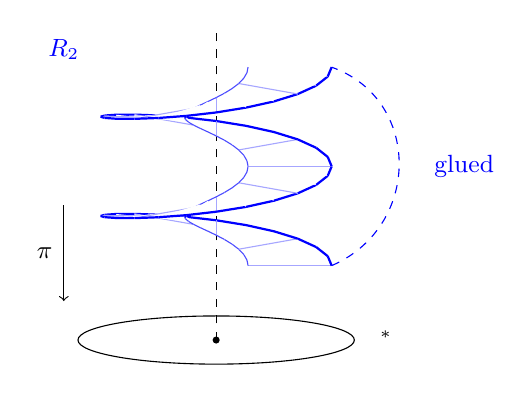
\begin{tikzpicture}[scale=0.9]
	\draw[thin] (0,-2.5) ellipse (1.95 and 0.34);
	\fill (0,-2.5) circle (0.05);
	\node at (2.4,-2.5) {\small $\Cs$};
	\draw[thin, dashed] (0,-2.5) -- (0,1.9);
	\foreach \t in {0,15,...,705} {
		\pgfmathsetmacro\tb{\t+15}
		\pgfmathsetmacro\ya{0.29*sin(\t) + \t*0.003889 - 1.45}
		\pgfmathsetmacro\yb{0.29*sin(\tb) + \tb*0.003889 - 1.45}
		\pgfmathsetmacro\yc{0.08*sin(\tb) + \tb*0.003889 - 1.45}
		\pgfmathsetmacro\yd{0.08*sin(\t) + \t*0.003889 - 1.45}
		\pgfmathtruncatemacro\sp{mod(\t,45)}
		\fill[white] ({1.63*cos(\t)},\ya) -- ({1.63*cos(\tb)},\yb) --
			({0.45*cos(\tb)},\yc) -- ({0.45*cos(\t)},\yd) -- cycle;
		\ifnum\sp=0
			\draw[color=blue!35, thin] ({1.63*cos(\t)},\ya) -- ({0.45*cos(\t)},\yd);
		\fi
		\draw[color=blue, thick] ({1.63*cos(\t)},\ya) -- ({1.63*cos(\tb)},\yb);
		\draw[color=blue!70, thin] ({0.45*cos(\t)},\yd) -- ({0.45*cos(\tb)},\yc);
	}
	% the bottom and top edges of the ramp are identified
	\draw[thin, color=blue, dashed] (1.63,-1.45) .. controls (2.9,-0.9) and (2.9,0.9) .. (1.63,1.35);
	\node[color=blue] at (3.5,-0.05) {\small glued};
	\draw[->, thin] (-2.15,-0.6) -- (-2.15,-1.95);
	\node at (-2.42,-1.28) {\small $\pi$};
	\node[color=blue] at (-2.15,1.6) {\small $R_2$};
\end{tikzpicture}
\end{center}

In both cases $g$ (respectively $f$) is the honest single-valued function we were after,
and $\pi$ is the map remembering which point of $\Cs$ we are sitting over. The key
structural feature of $\pi$ is that it is a \emph{local homeomorphism}: each little piece
of $R$ maps homeomorphically to a piece of $\Cs$. That is what will let us transport the
complex structure of $\Cs$ upstairs, and it is where we turn next.

\begin{remark}
	One thing is unsatisfactory about $R_k$: the interesting point $0$ is missing, and so
	is $\infty$. We would like to add them, obtaining a map
	$\hat{p}_k : \Cinf \to \Cinf$ which is $k$-to-$1$ everywhere except at the two points
	$0, \infty$, where it is $1$-to-$1$. These exceptional points are the \vocab{branch
	points}, and understanding them is the goal of Section \ref{sec:branching}. Once the
	points are added, $\pi$ is no longer a covering map -- but it is still holomorphic, and
	that turns out to be the more useful category.
\end{remark}

\section{Riemann Surfaces}

\subsection{Covering Maps}

We isolate the topological property of $\pi : R \to \Cs$ that made the last section work.
This material overlaps heavily with II Algebraic Topology; we repeat it because the
conventions differ slightly and because we shall need to be careful about exactly which
hypotheses are used where.

\begin{definition}[Covering Map]
	Let $\tilde X, X$ be path-connected Hausdorff spaces. A continuous surjection
	$\pi : \tilde X \to X$ is a \vocab{covering map} if it is a local homeomorphism: every
	$\tilde x \in \tilde X$ has an open neighbourhood $\tilde U$ such that $\pi|_{\tilde U}$
	is a homeomorphism onto an open subset of $X$.
\end{definition}

\begin{definition}[Regular Covering Map]
	A covering map $\pi : \tilde X \to X$ is \vocab{regular} if every $x \in X$ has an open
	neighbourhood $U$ which is \vocab{evenly covered}: there is a discrete set $\Delta$ and
	a homeomorphism $\pi^{-1}(U) \cong U \times \Delta$ under which $\pi$ becomes the
	projection $(u, \delta) \mapsto u$. Equivalently, $\pi^{-1}(U)$ is a disjoint union of
	open sets, the \vocab{sheets} over $U$, each mapped homeomorphically onto $U$ by $\pi$.
\end{definition}

\begin{center}
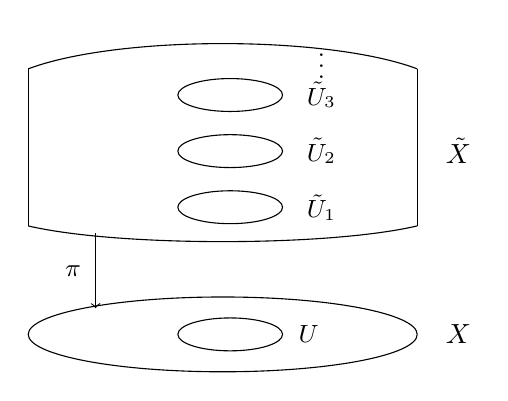
\begin{tikzpicture}[scale=0.95]
	\draw[thin] (0,0) ellipse (2.6 and 0.5);
	\node at (3.15,0) {$X$};
	\draw[thin] (0.1,0) ellipse (0.7 and 0.22);
	\node at (1.15,0) {\small $U$};
	\foreach \y in {1.7, 2.45, 3.2} { \draw[thin] (0.1,\y) ellipse (0.7 and 0.22); }
	\node at (1.32,1.7) {\small $\tilde U_1$};
	\node at (1.32,2.45) {\small $\tilde U_2$};
	\node at (1.32,3.2) {\small $\tilde U_3$};
	\node at (1.32,3.7) {\small $\vdots$};
	\node at (3.15,2.45) {$\tilde X$};
	\draw[thin] (-2.6,1.45) -- (-2.6,3.55);
	\draw[thin] (2.6,1.45) -- (2.6,3.55);
	\draw[thin] (-2.6,3.55) .. controls (-1.4,4.0) and (1.4,4.0) .. (2.6,3.55);
	\draw[thin] (-2.6,1.45) .. controls (-1.4,1.17) and (1.4,1.17) .. (2.6,1.45);
	\draw[->, thin] (-1.7,1.35) -- (-1.7,0.35);
	\node at (-2.0,0.85) {\small $\pi$};
\end{tikzpicture}
\end{center}

Regularity is a genuinely stronger condition, and it is the one that matters for lifting
paths. The distinction is easy to miss, so here are the examples we shall use.

\begin{example}\
	\begin{enumerate}[label=(\roman*)]
		\item The map $\pi : R \to \Cs$ of Section \ref{sec:logsurface} is a regular
		covering map. Indeed
		$$
		\pi^{-1}(U_n) = \coprod_{m \equiv n \ (4)} U_m \cong U_n \times \Z,
		$$
		since the copy $U_m$ maps homeomorphically to $U_n$ exactly when $m \equiv n$
		modulo $4$, and distinct such copies are disjoint in $R$.

		\item $\exp : \C \to \Cs$ is a regular covering map. For an open interval
		$I \subseteq \R$ of length at most $2\pi$, write $\tilde V_I = \R + iI$, a
		horizontal strip; then $\exp$ restricts to a homeomorphism $\tilde V_I \to U_I$
		with inverse a branch of $\log$, and
		$$
		\exp^{-1}(U_{I(n)}) = \coprod_{m \equiv n \ (4)} \tilde V_{I(m)} \cong U_{I(n)} \times \Z.
		$$

		\item $p_k : \Cs \to \Cs$, $z \mapsto z^k$, is a regular covering map with $k$
		sheets: over the sector $U_I$ with $I$ of length less than $2\pi/k$ sit the $k$
		sectors $\zeta^j U_{I/k}$, $\zeta = e^{2\pi i /k}$.

		\item \emph{(Non-example.)} The inclusion $\iota : \disc \hookrightarrow \C$ is a
		local homeomorphism, hence a covering map onto its image in the weak sense above,
		but it is not regular as a map to $\C$: for $z_0 \in \mathbb{T}$ and any
		neighbourhood $U$ of $z_0$, we have $\iota^{-1}(U) = U \cap \disc$, whose image is
		not $U$. More basically, $\iota$ is not surjective. Regularity is what rules out
		this kind of `partial' cover.
	\end{enumerate}
\end{example}

\subsection{Charts and Atlases}

Now we say what a surface is. The idea is Riemann's: a space that looks locally like an
open subset of $\C$, in a way that is compatible from patch to patch.

\begin{definition}[Chart]
	Let $R$ be a topological space. A \vocab{chart} on $R$ is a pair $(\phi, U)$ where
	$U \subseteq R$ is open and $\phi : U \to \phi(U) \subseteq \C$ is a homeomorphism
	onto an open subset of $\C$. We call $\phi$ a \vocab{local coordinate} on $U$.
\end{definition}

\begin{definition}[Atlas]
	A collection $\mathcal{A}$ of charts on $R$ is an \vocab{atlas} if
	\begin{enumerate}[label=(\roman*)]
		\item $\bigcup_{(\phi,U) \in \mathcal{A}} U = R$;
		\item for all $(\phi_1, U_1), (\phi_2, U_2) \in \mathcal{A}$ with
		$U_1 \cap U_2 \neq \emptyset$, the \vocab{transition function}
		$$
		\phi_1 \circ \phi_2^{-1} : \phi_2(U_1 \cap U_2) \to \phi_1(U_1 \cap U_2)
		$$
		is holomorphic.
	\end{enumerate}
\end{definition}

Note that the transition function goes between open subsets of $\C$, so `holomorphic'
means what it always meant. Note also that its inverse is $\phi_2 \circ \phi_1^{-1}$,
which is holomorphic by the same condition with the roles swapped; so transition functions
are automatically biholomorphic.

\begin{center}
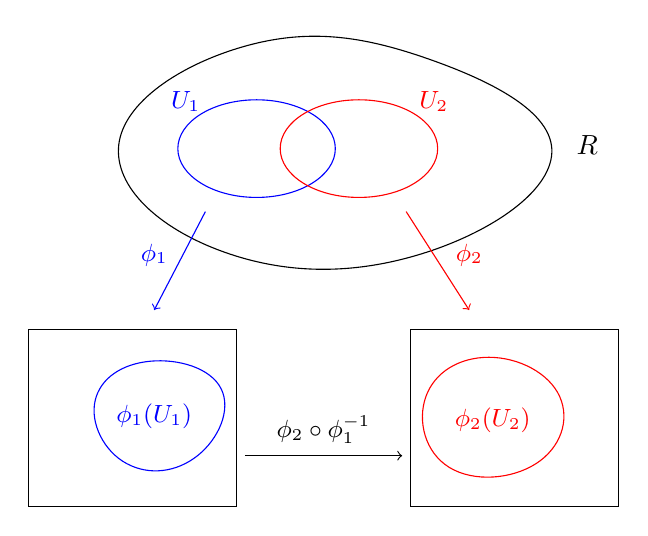
\begin{tikzpicture}[scale=1]
	% surface blob
	\draw[thin] plot[smooth cycle, tension=0.75] coordinates {(-2.6,0.5) (-1.0,1.75) (1.3,1.6) (2.9,0.4) (1.2,-0.9) (-1.3,-0.85)};
	\node at (3.35,0.5) {$R$};
	% two patches
	\draw[thin, color=blue] (-0.85,0.45) ellipse (1.0 and 0.62);
	\draw[thin, color=red] (0.45,0.45) ellipse (1.0 and 0.62);
	\node[color=blue] at (-1.75,1.05) {\small $U_1$};
	\node[color=red] at (1.4,1.05) {\small $U_2$};
	% images
	\begin{scope}[yshift=-3.1cm]
		\draw[thin, color=blue] plot[smooth cycle, tension=0.8] coordinates {(-2.9,0.35) (-2.2,0.85) (-1.3,0.5) (-1.6,-0.35) (-2.5,-0.45)};
		\node[color=blue] at (-2.15,0.15) {\small $\phi_1(U_1)$};
		\draw[thin, color=red] plot[smooth cycle, tension=0.8] coordinates {(1.3,0.4) (2.1,0.9) (3.0,0.4) (2.7,-0.45) (1.6,-0.5)};
		\node[color=red] at (2.15,0.1) {\small $\phi_2(U_2)$};
		\draw[thin] (-3.75,-1.0) rectangle (-1.1,1.25);
		\draw[thin] (1.1,-1.0) rectangle (3.75,1.25);
		\node at (-3.5,1.0) {\small $\C$};
		\node at (1.35,1.0) {\small $\C$};
	\end{scope}
	\draw[->, thin, color=blue] (-1.5,-0.35) -- (-2.15,-1.6);
	\node[color=blue] at (-2.15,-0.9) {\small $\phi_1$};
	\draw[->, thin, color=red] (1.05,-0.35) -- (1.85,-1.6);
	\node[color=red] at (1.85,-0.9) {\small $\phi_2$};
	\draw[->, thin] (-1.0,-3.45) -- (1.0,-3.45);
	\node at (0,-3.12) {\small $\phi_2 \circ \phi_1^{-1}$};
\end{tikzpicture}
\end{center}

There is an annoying redundancy here, which the next example exposes.

\begin{example}\label{ex:atlasesonC}
	Take $R = \C$. Let $\mathcal{A}$ consist of all pairs $(\id_U, U)$ for $U \subseteq \C$
	open; this is an atlas. Let $\mathcal{A}'$ consist of all pairs $(z \mapsto z + 1, U)$;
	this too is an atlas. So is $\mathcal{A} \cup \mathcal{A}'$, since the transition
	functions are translations. Yet all three describe the same complex analysis on $\C$.
\end{example}

The cure is to take the largest possible atlas, so that no information is hidden in a
choice.

\begin{definition}[Conformal Structure]
	A \vocab{conformal structure} on $R$ is an atlas $\mathcal{A}$ which is \vocab{maximal}:
	whenever a chart $(\psi, V)$ on $R$ has the property that $\phi \circ \psi^{-1}$ is
	holomorphic (where defined) for every $(\phi, U) \in \mathcal{A}$, we have
	$(\psi, V) \in \mathcal{A}$.
\end{definition}

\begin{definition}[Riemann Surface]
	A \vocab{Riemann surface} is a pair $(R, \mathcal{A})$ where $R$ is a path-connected
	Hausdorff topological space and $\mathcal{A}$ is a conformal structure on $R$.
\end{definition}

We will normally suppress $\mathcal{A}$ and just write $R$. Note that connectedness is
part of the definition here -- some authors allow disconnected Riemann surfaces, but for
us a Riemann surface is connected, which makes the identity theorem available at all
times.

Maximal atlases are unwieldy to write down, so in practice we always specify a small
atlas and appeal to the following.

\begin{lemma}\label{lem:atlasextends}
	Every atlas $\mathcal{A}$ on $R$ is contained in a unique conformal structure
	$\hat{\mathcal{A}}$.
\end{lemma}

\begin{proof}
	There is only one possible candidate: let $\hat{\mathcal{A}}$ be the set of all charts
	$(\psi, V)$ on $R$ such that $\psi \circ \phi^{-1}$ and $\phi \circ \psi^{-1}$ are
	holomorphic for every $(\phi, U) \in \mathcal{A}$. Any conformal structure containing
	$\mathcal{A}$ is contained in $\hat{\mathcal{A}}$ by definition of an atlas, and
	contains $\hat{\mathcal{A}}$ by maximality; so uniqueness is clear once we know
	$\hat{\mathcal{A}}$ is an atlas.

	It covers $R$ since $\mathcal{A} \subseteq \hat{\mathcal{A}}$ does. For compatibility,
	take $(\psi_1, V_1), (\psi_2, V_2) \in \hat{\mathcal{A}}$ and $p \in V_1 \cap V_2$.
	Choose $(\phi, U) \in \mathcal{A}$ with $p \in U$. Near $\psi_2(p)$ we may write
	$$
	\psi_1 \circ \psi_2^{-1} = (\psi_1 \circ \phi^{-1}) \circ (\phi \circ \psi_2^{-1}),
	$$
	a composite of holomorphic maps, hence holomorphic at $\psi_2(p)$. As $p$ was
	arbitrary, $\psi_1 \circ \psi_2^{-1}$ is holomorphic on $\psi_2(V_1 \cap V_2)$.
	Maximality of $\hat{\mathcal{A}}$ is immediate from its definition.
\end{proof}

So from now on, `here is an atlas' means `here is a Riemann surface'.

\subsection{First Examples}

\begin{example}[The Plane]
	Taking $\mathcal{A} = \{(\id, \C)\}$ and extending gives the \vocab{canonical
	conformal structure} on $\C$. Whenever we speak of $\C$ as a Riemann surface, this is
	what is meant. Note that by Example \ref{ex:atlasesonC} the atlas of all translations
	extends to the same structure.
\end{example}

\begin{example}[The Conjugate Plane]
	The single chart $(z \mapsto \bar z, \C)$ is also an atlas on $\C$, and it does
	\emph{not} extend to the canonical structure, since $z \mapsto \bar z$ is not
	holomorphic. Write $\bar\C$ for $\C$ with this structure. So the same topological
	space can carry different conformal structures. (As it happens $\bar \C \cong \C$ as
	Riemann surfaces, via $z \mapsto \bar z$ -- but they are not \emph{equal}.)
\end{example}

\begin{example}[Open Subsets]\label{ex:opensubset}
	If $R$ is a Riemann surface with conformal structure $\mathcal{A}$ and
	$S \subseteq R$ is open and connected, then
	$$
	\{ (\phi|_{U \cap S}, U \cap S) : (\phi, U) \in \mathcal{A} \}
	$$
	is an atlas on $S$, making $S$ a Riemann surface. In particular every domain
	$D \subseteq \C$ -- the disc $\disc$, the upper half-plane $\Hp$, the punctured plane
	$\Cs$ -- is a Riemann surface.
\end{example}

\begin{example}[The Riemann Sphere]\label{ex:sphere}
	Let $\Cinf = \C \cup \{\infty\}$ with the topology in which neighbourhoods of $\infty$
	are the complements of compact subsets of $\C$. Take the two charts
	$$
	(\phi_0, U_0) = (\id, \C), \qquad (\phi_1, U_1) = \left(z \mapsto 1/z, \ \Cs \cup \{\infty\}\right),
	$$
	where we read $1/\infty = 0$. Each is a homeomorphism onto $\C$, they cover $\Cinf$,
	and on the overlap $U_0 \cap U_1 = \Cs$ the transition function is $z \mapsto 1/z$,
	which is holomorphic there. So this is an atlas, and $\Cinf$ is a Riemann surface,
	the \vocab{Riemann sphere}.
\end{example}

That $\Cinf$ deserves to be called a sphere is the content of stereographic projection.
Identify $\C$ with the plane $\{x_3 = 0\}$ in $\R^3$ and let $S^2$ be the unit sphere,
with north pole $N = (0,0,1)$. Each point $P \in S^2 \setminus \{N\}$ determines a unique
point of the plane, namely where the line $NP$ meets it, and this gives a homeomorphism
$S^2 \setminus \{N\} \to \C$; sending $N \mapsto \infty$ extends it to a homeomorphism
$S^2 \to \Cinf$.

\begin{center}
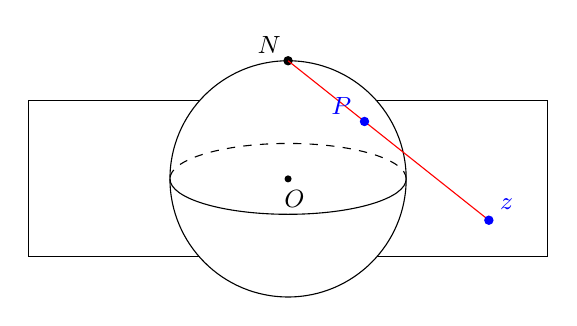
\begin{tikzpicture}[scale=1.5]
	% the plane x_3 = 0, in the projection (x,y,z) |-> (x, 0.3y + z)
	\draw[thin] (-2.2,-0.66) -- (2.2,-0.66) -- (2.2,0.66) -- (-2.2,0.66) -- cycle;
	\node at (-1.95,0.5) {\small $\C$};
	% sphere (filled so the plane does not show through it)
	\fill[white] (0,0) circle (1);
	\draw[thin] (0,0) circle (1);
	% equator: back half dashed, front half solid
	\draw[thin, dashed] (1,0) arc (0:180:1 and 0.3);
	\draw[thin] (-1,0) arc (180:360:1 and 0.3);
	% north pole
	\fill (0,1) circle (0.04);
	\node at (-0.16,1.13) {\small $N$};
	% the ray N -> z, meeting the sphere at P = (0.647,-0.444,0.619)
	\draw[thin, color=red] (0,1) -- (1.7,-0.35);
	\fill[color=blue] (0.647,0.486) circle (0.04);
	\node[color=blue] at (0.45,0.62) {\small $P$};
	\fill[color=blue] (1.7,-0.35) circle (0.04);
	\node[color=blue] at (1.85,-0.21) {\small $z$};
	\node at (0.055,-0.17) {\small $O$};
	\fill (0,0) circle (0.03);
\end{tikzpicture}
\end{center}

Chasing the geometry, if $P = (x_1,x_2,x_3)$ then the line $N + t(P - N)$ meets $x_3 = 0$
at $t = 1/(1-x_3)$, giving
$$
z = \frac{x_1 + i x_2}{1 - x_3}.
$$
Projecting instead from the south pole $S = (0,0,-1)$ gives $z' = (x_1 - ix_2)/(1 + x_3)$,
and one checks $z z' = 1$ using $x_1^2 + x_2^2 + x_3^2 = 1$. So the two stereographic
projections differ by $z \mapsto 1/z$ -- exactly the transition function of Example
\ref{ex:sphere}. The atlas we wrote down is the geometrically natural one.

\begin{remark}
	Under this identification, `$z \to \infty$' means `$P \to N$', so the point $\infty$
	is in no way special: the sphere has a transitive group of conformal automorphisms
	(the M\"obius transformations) and $\infty$ can be moved anywhere. That is the real
	payoff of the Riemann sphere as against the extended plane of a first course.
\end{remark}

\subsection{Holomorphic Maps}

\begin{definition}[Holomorphic Map]
	Let $R, S$ be Riemann surfaces. A continuous map $f : R \to S$ is
	\vocab{holomorphic} (or \vocab{analytic}) if for every chart $(\phi, U)$ on $R$ and
	every chart $(\psi, V)$ on $S$, the map
	$$
	\psi \circ f \circ \phi^{-1}
	$$
	is holomorphic on $\phi(U \cap f^{-1}(V))$.
\end{definition}

The composite $\psi \circ f \circ \phi^{-1}$ is called the \vocab{local expression} of
$f$ in the charts $\phi$ and $\psi$. Checking the condition for \emph{all} charts is of
course impossible in practice; happily it suffices to check one chart at each point.

\begin{lemma}\label{lem:holcheckone}
	A continuous map $f : R \to S$ is holomorphic if and only if for each $p \in R$ there
	exist charts $(\phi_p, U_p)$ on $R$ with $p \in U_p$ and $(\psi_p, V_p)$ on $S$ with
	$f(p) \in V_p$ such that $\psi_p \circ f \circ \phi_p^{-1}$ is holomorphic on
	$\phi_p(U_p \cap f^{-1}(V_p))$.
\end{lemma}

\begin{proof}
	Necessity is trivial. For sufficiency, let $(\phi, U)$ and $(\psi, V)$ be arbitrary
	charts; we must show $\psi \circ f \circ \phi^{-1}$ is holomorphic at $\phi(p)$ for
	each $p \in U \cap f^{-1}(V)$. Take $(\phi_p, U_p), (\psi_p, V_p)$ as hypothesised.
	On a small enough neighbourhood of $\phi(p)$ we may factor
	$$
	\psi \circ f \circ \phi^{-1} = (\psi \circ \psi_p^{-1}) \circ (\psi_p \circ f \circ \phi_p^{-1}) \circ (\phi_p \circ \phi^{-1}).
	$$
	The outer two factors are transition functions, hence holomorphic; the middle factor is
	holomorphic by hypothesis. So the composite is holomorphic at $\phi(p)$.
\end{proof}

\begin{lemma}\label{lem:compholo}
	If $f : R \to S$ and $g : S \to T$ are holomorphic, so is $g \circ f : R \to T$.
\end{lemma}

\begin{proof}
	Immediate from Lemma \ref{lem:holcheckone}: locally $g \circ f$ has local expression
	$(\chi \circ g \circ \psi^{-1}) \circ (\psi \circ f \circ \phi^{-1})$.
\end{proof}

\begin{definition}[Conformal Equivalence]
	A \vocab{conformal equivalence} (or \vocab{biholomorphism}) is a holomorphic bijection
	$f : R \to S$ whose inverse is holomorphic. We then write $R \cong S$.
\end{definition}

By Lemma \ref{lem:compholo} this is an equivalence relation on Riemann surfaces, and it is
the notion of sameness we care about. We will see later (Corollary \ref{cor:degree1}) that
the hypothesis on $f^{-1}$ is automatic: a holomorphic bijection of Riemann surfaces is
always a conformal equivalence.

\begin{example}
	The map $\C \to \bar\C$, $z \mapsto \bar z$, is a conformal equivalence: in the chart
	$\id$ upstairs and $z \mapsto \bar z$ downstairs, its local expression is
	$z \mapsto \overline{\bar z} = z$.
\end{example}

\begin{example}[M\"obius Maps]\label{ex:mobius}
	For $a,b,c,d \in \C$ with $ad - bc \neq 0$, the M\"obius transformation
	$$
	\mu(z) = \frac{az+b}{cz+d}, \qquad \mu(-d/c) = \infty, \quad \mu(\infty) = a/c
	$$
	is a conformal equivalence $\Cinf \to \Cinf$. Indeed $\mu$ is holomorphic away from
	$-d/c$ and $\infty$, and at those points one checks holomorphy in the chart $1/z$: for
	example near $z = \infty$ the local expression is
	$w \mapsto (cw + d)/(aw+b)$ (in the chart $w = 1/z$ upstairs and $1/z$ downstairs when
	$a \ne 0$), which is holomorphic at $0$. The inverse is again M\"obius. In fact
	\emph{every} conformal automorphism of $\Cinf$ is of this form, as we shall see.
\end{example}

\begin{example}[$\Cs$ and the Cylinder]
	The map $\C \to \Cs$, $z \mapsto e^z$, is holomorphic and surjective but not injective;
	it descends to a conformal equivalence $\C / 2\pi i \Z \to \Cs$ once we know how to
	give the quotient a conformal structure. That is the next subsection.
\end{example}

\subsection{Structures Induced by Covering Maps}

Here is the tool that lets us construct nearly all our examples: a covering of a Riemann
surface is a Riemann surface, in exactly one way.

\begin{lemma}\label{lem:coverstructure}
	Let $R$ be a Riemann surface and $\pi : \tilde R \to R$ a covering map, with
	$\tilde R$ path-connected and Hausdorff. Then there is a unique conformal structure on
	$\tilde R$ making $\pi$ holomorphic.
\end{lemma}

\begin{proof}
	\emph{Existence.} Let $p \in \tilde R$. Since $\pi$ is a local homeomorphism, choose an
	open $\tilde N \ni p$ mapped homeomorphically by $\pi$ onto an open $N \ni \pi(p)$.
	Choose a chart $(\phi, U)$ on $R$ with $\pi(p) \in U$, and set
	$$
	\tilde U = (\pi|_{\tilde N})^{-1}(N \cap U), \qquad
	\tilde\phi = \phi \circ \pi|_{\tilde U}.
	$$
	Then $\tilde \phi$ is a composite of homeomorphisms onto open subsets of $\C$, so
	$(\tilde\phi, \tilde U)$ is a chart, and these charts cover $\tilde R$. For two of them
	the transition function is
	$$
	\tilde\phi_1 \circ \tilde\phi_2^{-1} = \phi_1 \circ \pi \circ \pi^{-1} \circ \phi_2^{-1} = \phi_1 \circ \phi_2^{-1},
	$$
	(with the evident restrictions), which is holomorphic since $\phi_1, \phi_2$ came from
	an atlas on $R$. So we have an atlas, and by Lemma \ref{lem:atlasextends} a conformal
	structure $\tilde{\mathcal{A}}$.

	In this structure $\pi$ is holomorphic: with $\tilde\phi$ built from $\phi$ as above,
	the local expression of $\pi$ is
	$$
	\phi \circ \pi \circ \tilde\phi^{-1} = \phi\circ \pi \circ \pi^{-1} \circ \phi^{-1} = \id,
	$$
	and Lemma \ref{lem:holcheckone} applies.

	\emph{Uniqueness.} Let $\tilde{\mathcal{B}}$ be any conformal structure on $\tilde R$
	making $\pi$ holomorphic. If $(\psi, V) \in \tilde{\mathcal{B}}$ and $(\tilde\phi, \tilde U)$
	is one of the charts constructed above, then on the overlap
	$$
	\tilde\phi \circ \psi^{-1} = \phi \circ \pi \circ \psi^{-1}
	$$
	is holomorphic, being the local expression of $\pi$ in charts $\psi$ and $\phi$.
	Likewise $\psi \circ \tilde\phi^{-1}$ is holomorphic, since $\pi|_{\tilde U}$ has a
	holomorphic local inverse (its local expression is the identity). Hence every chart of
	$\tilde{\mathcal{B}}$ is compatible with our atlas, and by maximality
	$\tilde{\mathcal{B}} = \tilde{\mathcal{A}}$.
\end{proof}

\begin{example}[The Surface of the Logarithm, Again]
	Since $\pi : R \to \Cs$ is a covering map and $R$ is path-connected and Hausdorff,
	$R$ becomes a Riemann surface with $\pi$ holomorphic. Moreover $f : R \to \C$ is
	holomorphic, since locally $f|_{U_n} = f_n \circ \pi$ and $f_n$ is holomorphic.

	In fact we can identify $R$ outright. Each $f_n : U_n \to \tilde V_{I(n)} = \R + iI(n)$
	is a homeomorphism with inverse $\exp$, and these agree on overlaps by construction of
	$\sim$; so they patch to a bijection $f: R \to \C$, which is holomorphic with
	holomorphic inverse. Hence
	$$
	R \cong \C.
	$$
	The Riemann surface of the logarithm is just the plane -- but presented as a spiral
	over $\Cs$, with $\pi$ the map $\exp$ in disguise. This is our first hint that the
	interesting data is not the surface alone but the surface \emph{together with its map
	to the base}.
\end{example}

\begin{example}[The Surface of the $k$-th Root]
	Similarly $R_k$ becomes a Riemann surface with $\pi, g$ holomorphic, and $g : R_k \to \Cs$
	is a conformal equivalence, with $\pi = p_k \circ g$. So $R_k \cong \Cs$, again realised
	as a $k$-sheeted spiral over $\Cs$.
\end{example}

\subsection{Complex Tori}\label{subsec:tori}

So far our only compact example is $\Cinf$. Here is a family of others.

\begin{definition}[Lattice]
	Let $\omega_1, \omega_2 \in \Cs$ be linearly independent over $\R$. The subgroup
	$$
	\Lambda = \Z\omega_1 + \Z \omega_2 \leq (\C, +)
	$$
	is called a \vocab{lattice} in $\C$.
\end{definition}

\begin{center}
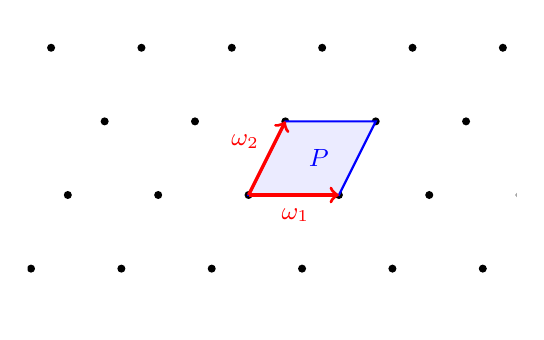
\begin{tikzpicture}[scale=0.85]
	\clip (-3.3,-1.75) rectangle (4.0,2.5);
	\foreach \m in {-4,-3,...,4} {
		\foreach \n in {-2,-1,0,1,2} {
			\fill ({\m*1.35 + \n*0.55}, {\n*1.1}) circle (0.06);
		}
	}
	% fundamental parallelogram
	\draw[thick, color=blue, fill=blue!8] (0,0) -- (1.35,0) -- (1.9,1.1) -- (0.55,1.1) -- cycle;
	\draw[->, very thick, color=red] (0,0) -- (1.35,0);
	\draw[->, very thick, color=red] (0,0) -- (0.55,1.1);
	\node[color=red] at (0.7,-0.3) {\small $\omega_1$};
	\node[color=red] at (-0.05,0.8) {\small $\omega_2$};
	\node[color=blue] at (1.05,0.55) {\small $P$};
\end{tikzpicture}
\end{center}

\begin{definition}[Complex Torus]
	The quotient group $T = \C/\Lambda$, with the quotient topology, is called a
	\vocab{complex torus}.
\end{definition}

The \vocab{fundamental parallelogram} $P = \{s\omega_1 + t\omega_2 : s, t \in [0,1]\}$
maps onto $T$, and is injective on its interior, so $T$ is compact (being a continuous
image of the compact set $P$) and indeed $T \cong S^1 \times S^1$ topologically, with the
two pairs of opposite edges of $P$ glued.

\begin{center}
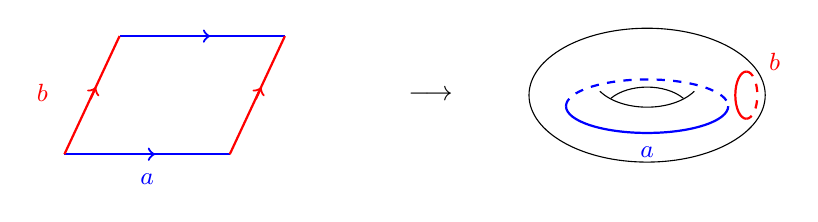
\begin{tikzpicture}[scale=1]
	% the parallelogram with identifications
	\draw[thick, color=blue] (0,0) -- (2.1,0);
	\draw[thick, color=blue] (0.7,1.5) -- (2.8,1.5);
	\draw[thick, color=red] (0,0) -- (0.7,1.5);
	\draw[thick, color=red] (2.1,0) -- (2.8,1.5);
	% arrows
	\foreach \s in {0,1} {
		\draw[->, thick, color=blue] ({1.0 + \s*0.7},{\s*1.5}) -- ({1.15+\s*0.7},{\s*1.5});
	}
	\foreach \s in {0,1} {
		\draw[->, thick, color=red] ({0.33+\s*2.1},{0.7}) -- ({0.4+\s*2.1},{0.85});
	}
	\node[color=blue] at (1.05,-0.32) {\small $a$};
	\node[color=red] at (-0.28,0.78) {\small $b$};
	\node at (4.65,0.75) {$\longrightarrow$};
	% torus
	\begin{scope}[xshift=7.4cm, yshift=0.75cm, scale=1.0]
		\draw[thin] (0,0) ellipse (1.5 and 0.85);
		\draw[thin] (-0.60,0.05) .. controls (-0.32,-0.22) and (0.32,-0.22) .. (0.60,0.05);
		\draw[thin] (-0.46,-0.04) .. controls (-0.23,0.15) and (0.23,0.15) .. (0.46,-0.04);
		% longitude a (blue): front solid, back dashed
		\draw[thick, color=blue] (-1.03,-0.14) arc (180:360:1.03 and 0.34);
		\draw[thick, color=blue, dashed] (-1.03,-0.14) arc (180:0:1.03 and 0.34);
		% meridian b (red)
		\draw[thick, color=red] (1.26,0.30) arc (90:270:0.14 and 0.30);
		\draw[thick, color=red, dashed] (1.26,0.30) arc (90:-90:0.14 and 0.30);
		\node[color=blue] at (0,-0.72) {\small $a$};
		\node[color=red] at (1.62,0.42) {\small $b$};
	\end{scope}
\end{tikzpicture}
\end{center}

We must give $T$ a conformal structure. Let $\pi : \C \to T$ be the quotient map.

\begin{proposition}\label{prop:torusstructure}
	$\pi : \C \to T$ is a regular covering map, and hence $T$ carries a unique conformal
	structure making $\pi$ holomorphic.
\end{proposition}

\begin{proof}
	First, $\Lambda$ is discrete: it is a lattice, so $\mu := \min\{|\lambda| : \lambda \in
	\Lambda \setminus \{0\}\}$ exists and is positive. (Indeed only finitely many lattice
	points lie in any bounded set, since $|m\omega_1 + n\omega_2| \geq c(|m| + |n|)$ for a
	constant $c > 0$ depending on $\omega_1, \omega_2$; we prove this in Lemma
	\ref{lem:latticesum}.) Fix $0 < \varepsilon < \mu/2$.

	$\pi$ is an open map, since for $U \subseteq \C$ open,
	$\pi^{-1}(\pi(U)) = \bigcup_{\lambda \in \Lambda}(U + \lambda)$ is open. Given
	$z_0 \in \C$, put $V = \pi(D(z_0,\varepsilon))$, which is open, and
	$$
	\pi^{-1}(V) = \bigcup_{\lambda\in\Lambda} (D(z_0,\varepsilon) + \lambda)
	= \coprod_{\lambda \in \Lambda} (D(z_0,\varepsilon)+\lambda),
	$$
	the union being disjoint because two of these discs meeting would give
	$|\lambda - \lambda'| < 2\varepsilon < \mu$. Each translate maps bijectively
	(hence homeomorphically, $\pi$ being open and continuous) onto $V$. So $\pi$ is a
	regular covering map, $\Lambda$ with the discrete topology indexing the sheets.

	$T$ is Hausdorff: given $\pi(z_0) \neq \pi(z_1)$, the sets $\pi(D(z_0,\delta))$ and
	$\pi(D(z_1,\delta))$ are disjoint open neighbourhoods once $2\delta$ is less than the
	distance from $z_1$ to $z_0 + \Lambda$. It is path-connected as a continuous image of
	$\C$. Now apply Lemma \ref{lem:coverstructure}.
\end{proof}

Explicitly, the charts on $T$ are the maps $(\pi|_{D(z_0,\varepsilon)})^{-1}$ defined on
$\pi(D(z_0,\varepsilon))$, and the transition functions are the translations
$z \mapsto z + \lambda$, which are certainly holomorphic. This is the cleanest possible
atlas, and it is why tori are such a good testing ground.

\begin{remark}
	All complex tori are homeomorphic, being homeomorphic to $S^1 \times S^1$. They are
	very far from being all conformally equivalent: one shows on the example sheets that
	$\C/\Lambda \cong \C/\Lambda'$ if and only if $\Lambda' = a\Lambda$ for some
	$a \in \Cs$, so that the conformal equivalence classes are parametrised by the modulus
	$\tau = \omega_2/\omega_1 \in \Hp$ up to the action of $\operatorname{SL}_2(\Z)$. There
	are uncountably many. So conformal structure is a strictly finer invariant than
	topology -- which is exactly why the subject is interesting.
\end{remark}

\section{Functions on Riemann Surfaces}

We have a supply of surfaces; now we do analysis on them. Every result in this section is
proved the same way: take charts, quote the corresponding theorem in $\C$, and check that
the conclusion is chart-independent. What makes the section worth reading is the
consequences, which are of a kind that has no analogue in the plane.

\subsection{The Identity Theorem}

\begin{theorem}[Identity Theorem for Riemann Surfaces]\label{thm:identityRS}
	Let $f, g : R \to S$ be holomorphic maps of Riemann surfaces. If the set
	$$
	A = \{p \in R : f(p) = g(p)\}
	$$
	has an accumulation point in $R$, then $f = g$.
\end{theorem}

\begin{proof}
	Let $B$ be the set of accumulation points of $A$ in $R$; by hypothesis $B \neq \emptyset$.
	We show $B$ is open and closed in $R$, which by connectedness gives $B = R$ and hence
	(as $A \supseteq B$ by continuity) $f = g$.

	\emph{$B$ is open.} Let $p \in B$. Then $f(p) = g(p) =: q$ by continuity. Choose a chart
	$(\psi, V)$ on $S$ about $q$ and a connected chart $(\phi, U)$ on $R$ about $p$ with
	$f(U), g(U) \subseteq V$; this is possible since $f, g$ are continuous. The local
	expressions $\psi f \phi^{-1}$ and $\psi g\phi^{-1}$ are holomorphic on the domain
	$\phi(U)$ and agree on a set with an accumulation point (namely $\phi(A \cap U)$, which
	accumulates at $\phi(p)$). By the identity theorem in $\C$ (Corollary \ref{cor:identity})
	they agree on $\phi(U)$, so $f = g$ on $U$, and every point of $U$ is an accumulation
	point of $A$. Hence $U \subseteq B$.

	\emph{$B$ is closed.} Suppose $p \in \bar B$. Take $U$ as above; $U$ meets $B$, so $U$
	contains points of $A$ other than $p$, whence by the argument above $f = g$ on $U$ and
	$p \in B$.
\end{proof}

\begin{corollary}\label{cor:notlocallyconstant}
	A non-constant holomorphic map $f : R \to S$ is nowhere locally constant, and its
	fibres $f^{-1}(q)$ are discrete.
\end{corollary}

\begin{proof}
	If $f$ were constant $= q$ on an open set, apply Theorem \ref{thm:identityRS} to $f$ and
	the constant map $q$. For the fibres: if $f^{-1}(q)$ had an accumulation point, the same
	comparison gives $f$ constant.
\end{proof}

\subsection{The Open Mapping Theorem}

\begin{theorem}[Open Mapping Theorem]\label{thm:omtRS}
	Every non-constant holomorphic map $f : R \to S$ of Riemann surfaces is an open map.
\end{theorem}

\begin{proof}
	Let $W \subseteq R$ be open and $p \in W$; we find a neighbourhood of $f(p)$ inside
	$f(W)$. Choose charts $(\phi, U)$ about $p$ and $(\psi, V)$ about $f(p)$, and shrink so
	that $U \subseteq W$, $U$ is connected and $f(U) \subseteq V$. By Corollary
	\ref{cor:notlocallyconstant} the local expression $F = \psi f \phi^{-1}$ is non-constant
	on the domain $\phi(U)$, so by the open mapping theorem in $\C$ (Theorem
	\ref{thm:omtplane}) $F(\phi(U))$ is open in $\C$. Hence
	$$
	f(U) = \psi^{-1}\left(F(\phi(U))\right)
	$$
	is open in $S$, being the preimage of an open set under the homeomorphism $\psi$
	restricted appropriately. As $f(U) \subseteq f(W)$ contains $f(p)$, we are done.
\end{proof}

\begin{corollary}\label{cor:compactsurjective}
	Let $f : R \to S$ be a non-constant holomorphic map with $R$ compact. Then $f$ is
	surjective and $S$ is compact.
\end{corollary}

\begin{proof}
	$f(R)$ is open by Theorem \ref{thm:omtRS} and compact as a continuous image of a
	compact set, hence closed since $S$ is Hausdorff. As $S$ is connected and $f(R)$ is a
	non-empty clopen subset, $f(R) = S$. Then $S = f(R)$ is compact.
\end{proof}

\begin{corollary}\label{cor:noholofnsoncompact}
	Every holomorphic function $f : R \to \C$ on a compact Riemann surface $R$ is constant.
\end{corollary}

\begin{proof}
	If $f$ were non-constant then $\C$ would be compact by Corollary
	\ref{cor:compactsurjective}. It is not.
\end{proof}

This is a striking statement, and it deserves to be dwelt on: it is a vast generalisation
of Liouville's theorem. On a compact surface there is \emph{no} interesting holomorphic
function at all. All the analysis on a compact Riemann surface must therefore be carried
by maps to other compact targets -- to $\Cinf$, giving meromorphic functions, or to other
surfaces. This single fact shapes the rest of the course.

\begin{theorem}[Maximum Modulus Principle]\label{thm:maxmodRS}
	Let $f : R \to \C$ be holomorphic on a Riemann surface. If $|f|$ attains a local
	maximum at some $p \in R$, then $f$ is constant.
\end{theorem}

\begin{proof}
	Suppose $f$ is non-constant, so $f(R)$ is open by Theorem \ref{thm:omtRS}. Let $W$ be a
	neighbourhood of $p$ with $|f(q)| \le |f(p)|$ for $q \in W$. Then $f(W)$ is an open
	neighbourhood of $f(p)$ contained in the closed disc $\overline{D}(0,|f(p)|)$; but every
	neighbourhood of $f(p)$ contains points of modulus greater than $|f(p)|$ (take
	$f(p)(1 + \epsilon)$ if $f(p) \ne 0$, or any small non-zero point if $f(p) = 0$). This
	is a contradiction.
\end{proof}

Combining these gives an alternative proof of Corollary \ref{cor:noholofnsoncompact}: on a
compact $R$ the continuous function $|f|$ attains a maximum, so $f$ is constant.

\subsection{Harmonic Functions}

The open mapping theorem tells us that a non-constant holomorphic function cannot be
real-valued, since $\R \subseteq \C$ has empty interior. Real-valued functions on Riemann
surfaces are therefore never holomorphic; the right class is the harmonic ones.

\begin{definition}[Harmonic Function]
	A smooth function $u : D \to \R$ on a domain $D \subseteq \C$ is \vocab{harmonic} if
	$$
	\nabla^2 u = \frac{\partial^2 u}{\partial x^2} + \frac{\partial^2 u}{\partial y^2} = 0.
	$$
\end{definition}

\begin{lemma}\label{lem:harmonicreal}
	Let $D \subseteq \C$ be a disc. A function $u : D \to \R$ is harmonic if and only if
	$u = \re f$ for some holomorphic $f$ on $D$.
\end{lemma}

\begin{proof}
	If $f = u + iv$ is holomorphic then the Cauchy--Riemann equations $u_x = v_y$,
	$u_y = -v_x$ give $u_{xx} + u_{yy} = v_{yx} - v_{xy} = 0$. The converse -- constructing
	a harmonic conjugate $v$ on a disc by integrating $-u_y\dd x + u_x \dd y$, which is
	closed by harmonicity and hence exact on a simply connected domain -- was an exercise
	in IB Complex Analysis.
\end{proof}

Note the appearance of simple connectedness: the converse fails on an annulus, as
$u = \log|z|$ shows.

\begin{definition}
	A function $u : R \to \R$ on a Riemann surface is \vocab{harmonic} if $u \circ \phi^{-1}$
	is harmonic for every chart $(\phi, U)$.
\end{definition}

For this to be a sensible definition we need harmonicity to be preserved by holomorphic
changes of coordinate, which it is:

\begin{lemma}\label{lem:harmoniconechart}
	A function $u : R \to \R$ is harmonic if and only if each $p \in R$ has \emph{some}
	chart $(\phi, U)$ with $p \in U$ and $u \circ \phi^{-1}$ harmonic.
\end{lemma}

\begin{proof}
	One direction is trivial. Conversely, suppose the condition holds and let $(\psi, V)$
	be any chart, $p \in V$. Choose $(\phi, U)$ as hypothesised with $p \in U$; shrinking,
	we may assume $\phi(U)$ is a disc, so $u\circ\phi^{-1} = \re f$ for some holomorphic $f$
	by Lemma \ref{lem:harmonicreal}. Then near $\psi(p)$,
	$$
	u \circ \psi^{-1} = (u \circ \phi^{-1})\circ(\phi\circ\psi^{-1}) = \re\left(f \circ (\phi \circ \psi^{-1})\right),
	$$
	the real part of a holomorphic function, hence harmonic.
\end{proof}

\begin{theorem}[Open Mapping and Identity Theorems for Harmonic Functions]
	Let $u, v$ be harmonic on a Riemann surface $R$.
	\begin{enumerate}[label=(\roman*)]
		\item If $\{p : u(p) = v(p)\}$ has non-empty interior then $u = v$.
		\item If $u$ is non-constant then $u : R \to \R$ is an open map.
	\end{enumerate}
	Consequently, every harmonic function on a compact Riemann surface is constant.
\end{theorem}

\begin{proof}
	Locally $u = \re f$ with $f$ holomorphic. For (i), if $u = v$ on an open set then
	locally $\re(f - g) = 0$, so $f - g$ is constant (its image lies in $i\R$, which has
	empty interior, so it cannot be open), and a clopen argument as in Theorem
	\ref{thm:identityRS} propagates this. For (ii), openness of $u$ follows from openness of
	$f$ on any chart where $f$ is non-constant, since $\re : \C \to \R$ is open. The last
	statement follows since $u(R)$ would be an open, compact -- hence clopen and non-empty
	-- subset of the connected space $\R$, forcing $u(R) = \R$, which is not compact.
\end{proof}

\subsection{Meromorphic Functions}

Since holomorphic functions to $\C$ are useless on compact surfaces, we enlarge the target
to the compact surface $\Cinf$.

\begin{definition}[Meromorphic Function]
	A \vocab{meromorphic function} on a Riemann surface $R$ is a holomorphic map
	$f : R \to \Cinf$ which is not identically $\infty$.
\end{definition}

Note that $f^{-1}(\infty)$ is then discrete by Corollary \ref{cor:notlocallyconstant}, and
closed since $\{\infty\}$ is; so a meromorphic function is a holomorphic function on the
complement of a discrete closed set. The next result confirms that on a plane domain this
agrees with the classical definition.

\begin{proposition}\label{prop:meroplane}
	Let $D \subseteq \C$ be a domain. A map $f : D \to \Cinf$ is meromorphic if and only if
	there is a discrete closed $A \subseteq D$ such that $f|_{D\setminus A}$ is holomorphic
	with values in $\C$, and $f$ has a pole at each point of $A$.
\end{proposition}

\begin{proof}
	($\Rightarrow$) Let $A = f^{-1}(\infty)$, which is discrete and closed as noted, and
	certainly $f$ is holomorphic $D \setminus A \to \C$. Fix $a \in A$ and work in the chart
	$w \mapsto 1/w$ about $\infty$. The local expression $z \mapsto 1/f(z)$ is holomorphic
	near $a$ and vanishes at $a$; it is not identically zero (else $f \equiv \infty$), so by
	Proposition \ref{prop:isolatedzeros} we may write $1/f(z) = (z-a)^m g(z)$ with $m \geq 1$
	and $g(a) \neq 0$. Shrinking so that $g$ has no zero, $f(z) = (z-a)^{-m}/g(z)$, which
	has a pole of order $m$ at $a$.

	($\Leftarrow$) $f$ is certainly holomorphic as a map into $\Cinf$ on $D \setminus A$.
	At $a \in A$ with a pole of order $m$ we may write $f(z) = (z-a)^{-m}h(z)$ with $h$
	holomorphic and $h(a)\neq 0$; then $1/f(z) = (z-a)^m/h(z)$ is holomorphic near $a$
	(after shrinking so $h$ does not vanish), and $f$ is continuous into $\Cinf$ at $a$
	since $|f| \to \infty$. So the local expression in the chart at $\infty$ is holomorphic,
	and Lemma \ref{lem:holcheckone} applies.
\end{proof}

\begin{example}
	The map $\Cinf \to \Cinf$ given by a rational function $p(z)/q(z)$ (in lowest terms,
	with the evident values at the zeros of $q$ and at $\infty$) is meromorphic. We shall
	see in Section \ref{sec:elliptic} that these are the \emph{only} meromorphic functions
	on $\Cinf$.
\end{example}

\begin{example}
	On a complex torus $T = \C/\Lambda$, a meromorphic function pulls back along
	$\pi : \C \to T$ to a meromorphic function on $\C$ invariant under $\Lambda$ -- that
	is, to a doubly periodic, or \vocab{elliptic}, function. Conversely every such function
	descends. Corollary \ref{cor:noholofnsoncompact} then says: a doubly periodic
	\emph{holomorphic} function on $\C$ is constant, which is Liouville's theorem applied
	to the (bounded, by compactness of $P$) function. Section \ref{sec:elliptic} is devoted
	to the non-constant ones.
\end{example}

\section{Covering Spaces and Monodromy}

To organise analytic continuation we need the topology of covering spaces. Most of this
was proved in II Algebraic Topology, and we shall be brisk, but the path-lifting and
homotopy-lifting statements are so central that it is worth seeing the proofs again in
the form we need.

\subsection{Lifting}

\begin{definition}[Lift]
	Let $\pi : \tilde X \to X$ be a covering map and $\gamma : [0,1] \to X$ a path. A
	\vocab{lift} of $\gamma$ is a path $\tilde \gamma : [0,1] \to \tilde X$ with
	$\pi \circ \tilde\gamma = \gamma$.
\end{definition}

\begin{example}
	For $\exp : \C \to \Cs$ and $\gamma(t) = e^{2\pi i t}$, both $t \mapsto 2\pi i t$ and
	$t \mapsto 2\pi i + 2\pi i t$ are lifts. They differ, but they start at different
	points -- and that is the general phenomenon.
\end{example}

\begin{proposition}[Uniqueness of Lifts]\label{prop:liftunique}
	Let $\pi : \tilde X \to X$ be a covering map and $\tilde\gamma_1, \tilde\gamma_2$ lifts
	of the same path $\gamma$. If $\tilde\gamma_1(0) = \tilde\gamma_2(0)$ then
	$\tilde\gamma_1 = \tilde\gamma_2$.
\end{proposition}

\begin{proof}
	Let $I = \{t \in [0,1] : \tilde\gamma_1(t) = \tilde\gamma_2(t)\}$, which is non-empty
	and closed (as $\tilde X$ is Hausdorff and the $\tilde \gamma_i$ continuous). We show
	$I$ is open, so that $I = [0,1]$ by connectedness.

	Let $t \in I$ and put $\tilde x = \tilde \gamma_1(t) = \tilde\gamma_2(t)$. As $\pi$ is
	a local homeomorphism there is an open $\tilde N \ni \tilde x$ with $\pi|_{\tilde N}$ a
	homeomorphism onto an open $N$. By continuity there is $\delta > 0$ with
	$\tilde\gamma_i((t-\delta, t+\delta)) \subseteq \tilde N$ for $i = 1,2$. For such $s$,
	$$
	\tilde\gamma_1(s) = (\pi|_{\tilde N})^{-1}(\gamma(s)) = \tilde\gamma_2(s),
	$$
	so $(t - \delta, t+\delta) \cap [0,1] \subseteq I$.
\end{proof}

Existence, however, requires regularity.

\begin{example}
	Let $\tilde X = \R + i(-\pi, 2\pi)$ and $\pi = \exp|_{\tilde X} : \tilde X \to \Cs$.
	This is a covering map (a local homeomorphism onto $\Cs$), but the loop
	$t \mapsto e^{2\pi i t}$ cannot be lifted starting at $0$: the lift would have to be
	$t \mapsto 2\pi i t$, which leaves $\tilde X$ at $t=1$. The map $\pi$ is not regular.
\end{example}

\begin{proposition}[Path Lifting]\label{prop:pathlifting}
	Let $\pi : \tilde X \to X$ be a regular covering map, $\gamma : [0,1] \to X$ a path
	and $\tilde x \in \tilde X$ with $\pi(\tilde x) = \gamma(0)$. Then there is a unique
	lift $\tilde\gamma$ of $\gamma$ with $\tilde\gamma(0) = \tilde x$.
\end{proposition}

\begin{proof}
	Uniqueness is Proposition \ref{prop:liftunique}. For existence let
	$$
	I = \{ t \in [0,1] : \gamma|_{[0,t]} \text{ lifts to some } \tilde\gamma \text{ with } \tilde\gamma(0) = \tilde x\},
	$$
	which contains $0$. Note that by uniqueness, lifts on $[0,t]$ for varying $t$ are
	compatible, so $I$ is an interval and the lifts patch.

	\emph{$I$ is open in $[0,1]$.} Let $\tau \in I$ with lift $\tilde\gamma$ on $[0,\tau]$.
	Choose an evenly covered $U \ni \gamma(\tau)$, so $\pi^{-1}(U) = \coprod_\delta U_\delta$,
	and let $U_{\delta_0}$ be the sheet containing $\tilde\gamma(\tau)$. Choose
	$\varepsilon > 0$ with $\gamma((\tau - \varepsilon, \tau+\varepsilon)) \subseteq U$;
	then setting $\tilde\gamma(t) = (\pi|_{U_{\delta_0}})^{-1}(\gamma(t))$ for
	$t \in [\tau, \tau + \varepsilon)$ extends the lift.

	\emph{$I$ is closed.} Let $\tau = \sup I$ and choose an evenly covered $U \ni \gamma(\tau)$
	with sheets $U_\delta$. Pick $\varepsilon > 0$ with
	$\gamma((\tau-\varepsilon,\tau]) \subseteq U$ and choose $t \in I$ with
	$t > \tau - \varepsilon$. The connected set $\tilde\gamma((\tau - \varepsilon, t])$ lies
	in $\pi^{-1}(U)$, hence in a single sheet $U_{\delta_0}$, and we may define
	$\tilde\gamma(s) = (\pi|_{U_{\delta_0}})^{-1}(\gamma(s))$ for
	$s \in (\tau - \varepsilon, \tau]$, which agrees with the existing lift and extends it
	continuously to $\tau$. So $\tau \in I$.

	Hence $I$ is a non-empty clopen subset of $[0,1]$, so $I = [0,1]$.
\end{proof}

\begin{theorem}[Homotopy Lifting, or the Monodromy Theorem]\label{thm:homotopylifting}
	Let $\pi : \tilde X \to X$ be a regular covering map and let $\alpha \simeq \beta$ be
	homotopic paths in $X$ (rel endpoints). Let $\tilde\alpha, \tilde\beta$ be their lifts
	with $\tilde\alpha(0) = \tilde\beta(0)$. Then $\tilde\alpha \simeq \tilde\beta$; in
	particular $\tilde\alpha(1) = \tilde\beta(1)$.
\end{theorem}

\begin{proof}
	This is the homotopy lifting property, proved in II Algebraic Topology: one lifts the
	homotopy $H : [0,1]^2 \to X$ by subdividing the square into small squares each mapping
	into an evenly covered set, and lifting them one at a time, using uniqueness of lifts to
	see the pieces agree. The resulting $\tilde H$ is a homotopy from $\tilde\alpha$ to
	$\tilde\beta$; since $H$ is constant on the two vertical edges, $\tilde H$ is too (a
	lift of a constant path is constant, by uniqueness), so the homotopy is rel endpoints.
\end{proof}

The name `monodromy theorem' attached to this statement is traditional and slightly
unfortunate, since we shall also use it for the classical statement about analytic
continuation (Theorem \ref{thm:classicalmonodromy}). The latter is a corollary of the
former, and the two are best regarded as the same theorem stated on either side of the
dictionary we are about to build.

\subsection{The Monodromy Group}

Let $\pi : \tilde X \to X$ be a regular covering map and fix a basepoint $x_0 \in X$. For
a loop $\gamma$ at $x_0$ and $\tilde x \in \pi^{-1}(x_0)$, let $\tilde\gamma_{\tilde x}$
be the lift starting at $\tilde x$; since $\pi(\tilde\gamma_{\tilde x}(1)) = \gamma(1) = x_0$,
the endpoint again lies in the fibre.

\begin{definition}[Monodromy Action]
	Define $\sigma_\gamma : \pi^{-1}(x_0) \to \pi^{-1}(x_0)$ by
	$\sigma_\gamma(\tilde x) = \tilde\gamma_{\tilde x}(1)$.
\end{definition}

\begin{center}
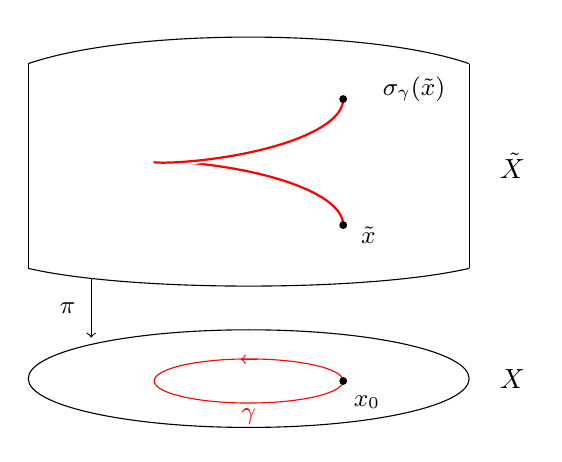
\begin{tikzpicture}[scale=1]
	% base
	\draw[thin] (0,0) ellipse (2.8 and 0.62);
	\node at (3.35,0) {$X$};
	\draw[thin, color=red] (0,-0.03) ellipse (1.2 and 0.28);
	\draw[->, thin, color=red] (0.1,0.245) -- (-0.1,0.245);
	\fill (1.2,-0.03) circle (0.05);
	\node at (1.5,-0.3) {\small $x_0$};
	\node[color=red] at (0,-0.48) {\small $\gamma$};
	% cover
	\draw[thin] (-2.8,1.4) -- (-2.8,4.0);
	\draw[thin] (2.8,1.4) -- (2.8,4.0);
	\draw[thin] (-2.8,4.0) .. controls (-1.5,4.45) and (1.5,4.45) .. (2.8,4.0);
	\draw[thin] (-2.8,1.4) .. controls (-1.5,1.1) and (1.5,1.1) .. (2.8,1.4);
	\node at (3.35,2.7) {$\tilde X$};
	% lifted path: back half first, then front half with a white halo so it reads
	% as passing in front
	\draw[thick, color=red, samples=120, domain=0:180, smooth, variable=\t]
		plot ({1.2*cos(\t)}, {0.28*sin(\t) + 1.95 + \t/360*1.6});
	\draw[line width=2.2pt, color=white, samples=120, domain=180:360, smooth, variable=\t]
		plot ({1.2*cos(\t)}, {0.28*sin(\t) + 1.95 + \t/360*1.6});
	\draw[thick, color=red, samples=120, domain=180:360, smooth, variable=\t]
		plot ({1.2*cos(\t)}, {0.28*sin(\t) + 1.95 + \t/360*1.6});
	\fill (1.2,1.95) circle (0.05);
	\node at (1.52,1.82) {\small $\tilde x$};
	\fill (1.2,3.55) circle (0.05);
	\node at (2.1,3.68) {\small $\sigma_\gamma(\tilde x)$};
	\draw[->, thin] (-2.0,1.28) -- (-2.0,0.52);
	\node at (-2.3,0.9) {\small $\pi$};
\end{tikzpicture}
\end{center}

\begin{proposition}
	The assignment $\gamma \mapsto \sigma_\gamma$ satisfies:
	\begin{enumerate}[label=(\roman*)]
		\item $\sigma_{c} = \id$ for the constant loop $c$;
		\item $\sigma_{\bar\gamma} = \sigma_\gamma^{-1}$, where $\bar\gamma(t) = \gamma(1-t)$;
		in particular each $\sigma_\gamma$ is a bijection;
		\item $\sigma_{\alpha \cdot \beta} = \sigma_\beta \circ \sigma_\alpha$;
		\item if $\alpha \simeq \beta$ then $\sigma_\alpha = \sigma_\beta$.
	\end{enumerate}
	Hence $\{\sigma_\gamma\}$ is a subgroup of $\sym(\pi^{-1}(x_0))$, and there is a
	well-defined (right) action of $\pi_1(X, x_0)$ on the fibre.
\end{proposition}

\begin{proof}
	(i) is clear. For (iii), if $\tilde\alpha_{\tilde x}$ is the lift of $\alpha$ at
	$\tilde x$, then the concatenation $\tilde\alpha_{\tilde x} \cdot
	\tilde\beta_{\tilde\alpha_{\tilde x}(1)}$ is a lift of $\alpha\cdot\beta$ starting at
	$\tilde x$, so by uniqueness it is \emph{the} lift, and its endpoint is
	$\sigma_\beta(\sigma_\alpha(\tilde x))$. Then (ii) follows from (i) and (iii). Finally
	(iv) is Theorem \ref{thm:homotopylifting}.
\end{proof}

\begin{definition}[Monodromy Group]
	The subgroup $\{\sigma_\gamma : \gamma \text{ a loop at } x_0\} \leq \sym(\pi^{-1}(x_0))$
	is the \vocab{monodromy group} of the covering $\pi$.
\end{definition}

Up to isomorphism it does not depend on the basepoint, since a path from $x_0$ to $x_1$
conjugates the two actions.

\begin{example}\label{ex:monodromypk}
	Take $p_k : \Cs \to \Cs$, $z \mapsto z^k$, with basepoint $1$. The fibre is the set of
	$k$-th roots of unity $\zeta^n$, $\zeta = e^{2\pi i /k}$. Let $\gamma(t) = e^{2\pi i t}$
	be the standard loop; its lift starting at $\zeta^n$ is
	$t \mapsto \zeta^n e^{2\pi i t /k}$, which ends at $\zeta^{n+1}$. So $\sigma_\gamma$ is
	the $k$-cycle $\zeta^n \mapsto \zeta^{n+1}$. Since $\pi_1(\Cs) \cong \Z$ is generated by
	$[\gamma]$, the monodromy group is cyclic of order $k$.

	This is the precise sense in which `$\sqrt[k]{z}$ has $k$ branches which are permuted
	cyclically as $z$ winds once round $0$'.
\end{example}

\begin{example}
	For $\exp : \C \to \Cs$ with basepoint $1$, the fibre is $2\pi i \Z$, the loop $\gamma$
	lifts to $t \mapsto 2\pi i t + 2\pi i n$ starting at $2\pi i n$, and
	$\sigma_\gamma$ is the shift $2\pi i n \mapsto 2\pi i (n+1)$. The monodromy group is
	infinite cyclic, matching the infinitely many branches of $\log$.
\end{example}

\section{The Space of Germs}\label{sec:germs}

We now build, once and for all, the Riemann surface on which a complete analytic function
becomes single-valued. The construction of Section \ref{sec:logsurface} was ad hoc: we
chose particular sectors and glued them by hand. The trick is to stop choosing. Take
\emph{all} function elements at once, remember only their local behaviour, and let the
topology sort things out.

\subsection{Germs}

Fix a domain $D \subseteq \C$.

\begin{definition}[Germ]
	Let $(f, U)$ and $(g, V)$ be function elements on $D$ and let $z \in U \cap V$. Write
	$(f,U) \equiv_z (g,V)$ if $f = g$ on some neighbourhood of $z$. This is an equivalence
	relation on the function elements whose domain contains $z$; the equivalence class of
	$(f,U)$ is the \vocab{germ} of $f$ at $z$, written $[f]_z$.
\end{definition}

So $[f]_z = [g]_w$ if and only if $z = w$ and $f, g$ agree near $z$. A germ at $z$ is
exactly the same data as a convergent power series centred at $z$; but the geometric
language will be more useful.

\begin{definition}[The Space of Germs]
	The \vocab{space of germs} over $D$ is
	$$
	\mathcal{G} = \mathcal{G}_D = \{[f]_z : z \in D, \ (f,U) \text{ a function element on } D \text{ with } z \in U\}.
	$$
\end{definition}

We topologise $\mathcal{G}$ so that germs of the same function at nearby points are
nearby. For a function element $(f,U)$ write
$$
[f]_U = \{[f]_z : z \in U\} \subseteq \mathcal{G},
$$
a `sheet' of germs.

\begin{lemma}
	The collection $\{[f]_U\}$, over all function elements $(f,U)$ on $D$, is a basis for a
	topology on $\mathcal{G}$.
\end{lemma}

\begin{proof}
	The sets cover $\mathcal{G}$ by definition. Suppose $[h]_z \in [f]_U \cap [g]_V$. Then
	$h$ agrees with $f$ near $z$ and with $g$ near $z$, so on some open $W \ni z$ with
	$W \subseteq U \cap V$ we have $h = f = g$, whence
	$[h]_W \subseteq [f]_U \cap [g]_V$ and $[h]_z \in [h]_W$.
\end{proof}

\begin{lemma}\label{lem:germshausdorff}
	$\mathcal{G}$ is Hausdorff.
\end{lemma}

\begin{proof}
	Let $[f]_z \neq [g]_w$. If $z \neq w$, choose disjoint neighbourhoods $U \ni z$,
	$V \ni w$ inside the domains of $f$ and $g$; then $[f]_U$ and $[g]_V$ are disjoint,
	since germs in them sit over disjoint sets of points.

	If $z = w$, choose a \emph{connected} open $U \ni z$ contained in both domains, so that
	$(f, U)$ and $(g,U)$ represent $[f]_z, [g]_z$. Suppose $[h]_y \in [f]_U \cap [g]_U$.
	Then $h$ agrees with $f$ near $y$ and with $g$ near $y$, so $f = g$ on a neighbourhood
	of $y$, and hence on all of $U$ by the identity theorem ($U$ being connected). But then
	$[f]_z = [g]_z$, a contradiction. So $[f]_U \cap [g]_U = \emptyset$.
\end{proof}

\begin{definition}
	The \vocab{forgetful map} $\pi : \mathcal{G} \to D$ is $\pi([f]_z) = z$.
\end{definition}

\begin{lemma}\label{lem:germscover}
	For each connected component $G$ of $\mathcal{G}$, the restriction $\pi : G \to D$ is a
	covering map onto its image, which is open in $D$. In particular $\pi$ is a local
	homeomorphism.
\end{lemma}

\begin{proof}
	$\pi$ is continuous: for $U \subseteq D$ open, $\pi^{-1}(U) = \bigcup [f]_{V}$ over all
	function elements $(f,V)$ with $V \subseteq U$, which is open. On a basic open set,
	$\pi|_{[f]_U} : [f]_U \to U$ is a bijection with inverse $z \mapsto [f]_z$, and this
	inverse is continuous because the preimage of a basic set $[g]_V$ is the open set
	$\{z \in U \cap V : f = g \text{ near } z\}$. So $\pi|_{[f]_U}$ is a homeomorphism onto
	the open set $U$, and $\pi$ is a local homeomorphism. Its image is therefore open, and
	each component $G$ of $\mathcal{G}$ is path-connected (being locally homeomorphic to
	open subsets of $\C$, hence locally path-connected) and Hausdorff by Lemma
	\ref{lem:germshausdorff}.
\end{proof}

\begin{remark}
	Note that $\pi : G \to D$ need not be \emph{regular}. For instance, take $D = \C$ and
	the component containing the germs of $z \mapsto 1/(1-z)$: continuation is blocked at
	$z=1$, and the fibre over $1$ can be empty while nearby fibres are not. This is exactly
	the phenomenon of a function element which cannot be continued along every path.
\end{remark}

By Lemma \ref{lem:coverstructure}, each component $G$ of $\mathcal{G}$ inherits a unique
conformal structure making $\pi$ holomorphic. Explicitly, the charts are the maps
$\pi|_{[f]_U}$ on the sets $[f]_U$, and the transition functions are identities. And
there is a canonical holomorphic function on it:

\begin{definition}[Evaluation Map]
	The \vocab{evaluation map} $E : \mathcal{G} \to \C$ is $E([f]_z) = f(z)$.
\end{definition}

This is well defined, since germs which agree near $z$ certainly agree at $z$. In the
chart $\pi|_{[f]_U}$ its local expression is
$$
E \circ (\pi|_{[f]_U})^{-1}(z) = E([f]_z) = f(z),
$$
which is holomorphic. So $E$ is a holomorphic function on $\mathcal{G}$.

This is the whole point. The multi-valued function has become the pair $(\pi, E)$: $\pi$
remembers which point of $D$ we are over, and $E$ is a genuine single-valued holomorphic
function.

\subsection{Analytic Continuation as Lifting}

Now we cash in.

\begin{theorem}\label{thm:contislifting}
	Let $(f,U), (g,V)$ be function elements on a domain $D$ and let $\gamma : [0,1] \to D$
	be a path with $\gamma(0) \in U$, $\gamma(1) \in V$. Then
	$$
	(f,U) \approx_\gamma (g,V) \iff \gamma \text{ lifts along } \pi \text{ to a path in } \mathcal{G} \text{ from } [f]_{\gamma(0)} \text{ to } [g]_{\gamma(1)}.
	$$
\end{theorem}

\begin{proof}
	($\Rightarrow$) Suppose we have a chain $(f,U) = (f_1,U_1) \sim \cdots \sim (f_n,U_n) = (g,V)$
	and a dissection $0 = t_0 < \cdots < t_n = 1$ with $\gamma([t_{i-1},t_i]) \subseteq U_i$.
	Define
	$$
	\tilde\gamma(t) = [f_i]_{\gamma(t)}, \qquad t \in [t_{i-1}, t_i].
	$$
	This is well defined at the joins: at $t = t_i$ we need $[f_i]_{\gamma(t_i)} =
	[f_{i+1}]_{\gamma(t_i)}$, which holds since $f_i = f_{i+1}$ on $U_i \cap U_{i+1}$, an
	open set containing $\gamma(t_i)$. On each $[t_{i-1},t_i]$ we have
	$\tilde\gamma = (\pi|_{[f_i]_{U_i}})^{-1}\circ\gamma$, which is continuous; by the
	gluing lemma $\tilde\gamma$ is continuous. Clearly $\pi \circ \tilde\gamma = \gamma$
	and the endpoints are as claimed.

	($\Leftarrow$) Suppose $\tilde\gamma$ is such a lift. Every point $\tilde\gamma(t)$ has
	a basic neighbourhood $[f_t]_{U_t}$ with $U_t$ a \emph{disc}. By compactness of $[0,1]$
	and the Lebesgue number lemma, there is a dissection
	$0 = t_0 < \cdots < t_n = 1$ and function elements $(f_i, U_i)$ with $U_i$ a disc and
	$\tilde\gamma([t_{i-1},t_i]) \subseteq [f_i]_{U_i}$. Applying $\pi$ gives
	$\gamma([t_{i-1},t_i]) \subseteq U_i$. Moreover for each $i$,
	$$
	[f_i]_{\gamma(t_i)} = \tilde\gamma(t_i) = [f_{i+1}]_{\gamma(t_i)},
	$$
	so $f_i = f_{i+1}$ near $\gamma(t_i) \in U_i \cap U_{i+1}$. Since $U_i, U_{i+1}$ are
	discs, $U_i \cap U_{i+1}$ is convex hence connected, and the identity theorem gives
	$f_i = f_{i+1}$ on $U_i \cap U_{i+1}$, i.e.\ $(f_i,U_i)\sim(f_{i+1},U_{i+1})$. Finally
	$[f_1]_{\gamma(0)} = [f]_{\gamma(0)}$ and $[f_n]_{\gamma(1)} = [g]_{\gamma(1)}$, and the
	identity theorem on the connected sets $U_1 \cap U$ and $U_n \cap V$ upgrades these germ
	equalities to $(f,U)\sim(f_1,U_1)$ and $(f_n,U_n)\sim(g,V)$.
\end{proof}

This is the theorem that makes the space of germs worth building: \emph{analytic
continuation along a path is path lifting}. Every fact about continuation is now a fact
about covering spaces.

\begin{corollary}\label{cor:completefn}
	Let $\mathcal{F}$ be a complete analytic function on a domain $D$. Then
	$$
	G_{\mathcal{F}} = \bigcup_{(f,U) \in \mathcal{F}} [f]_U
	$$
	is a path component of $\mathcal{G}$.
\end{corollary}

\begin{proof}
	Two germs lie in the same path component precisely when there is a path in
	$\mathcal{G}$ between them, which by Theorem \ref{thm:contislifting} happens precisely
	when the corresponding function elements are analytic continuations of one another.
\end{proof}

\begin{definition}
	$G_{\mathcal{F}}$, with the conformal structure of Lemma \ref{lem:coverstructure}, is
	\vocab{the Riemann surface of the complete analytic function} $\mathcal{F}$, equipped
	with $\pi : G_\mathcal{F} \to D$ and $E : G_\mathcal{F} \to \C$.
\end{definition}

\begin{example}
	Take $D = \Cs$ and $\mathcal{F}$ the complete analytic function containing the elements
	$F_n = (f_n, U_n)$ of Section \ref{subsec:logelements}. Then $G_\mathcal{F}$ is
	precisely the surface $R$ we built by hand, and $E$ is the function $f$. Indeed
	$\Phi : R \to G_\mathcal{F}$, $[z] \mapsto [f_n]_z$ for $z \in U_n$, is a well-defined
	homeomorphism commuting with the projections.
\end{example}

\subsection{The Classical Monodromy Theorem}

\begin{theorem}[Classical Monodromy Theorem]\label{thm:classicalmonodromy}
	Let $D \subseteq \C$ be a domain and $(f, U)$ a function element on $D$ which can be
	continued along \emph{every} path in $D$ starting in $U$. Suppose $\alpha, \beta$ are
	homotopic paths in $D$ (rel endpoints) from a point of $U$ to a point of $V$, and
	$$
	(f, U) \approx_\alpha (g_1, V), \qquad (f,U)\approx_\beta (g_2, V).
	$$
	Then $g_1 = g_2$ on $V$ (assuming $V$ connected).
\end{theorem}

\begin{proof}
	Let $G$ be the path component of $\mathcal{G}$ containing $[f]_{\alpha(0)}$. The
	hypothesis says exactly that every path in $D$ starting at $\alpha(0)$ lifts to $G$
	starting at $[f]_{\alpha(0)}$, from which one deduces that $\pi : G \to D$ is a regular
	covering map: given $z \in D$, take a disc $B \ni z$ in $D$; each germ in $\pi^{-1}(z)$
	extends over $B$ (continue along radii and use the identity theorem, or note that by
	Theorem \ref{thm:contislifting} the radial paths lift), giving a sheet of $\pi^{-1}(B)$
	over $B$, and these sheets are disjoint and exhaust $\pi^{-1}(B)$.

	Now let $\tilde\alpha, \tilde\beta$ be the lifts of $\alpha,\beta$ starting at
	$[f]_{\alpha(0)}$, which exist by Theorem \ref{thm:contislifting} and end at
	$[g_1]_{\alpha(1)}$, $[g_2]_{\beta(1)}$ respectively. Since $\alpha\simeq\beta$,
	Theorem \ref{thm:homotopylifting} gives $\tilde\alpha(1) = \tilde\beta(1)$, i.e.
	$$
	[g_1]_{\alpha(1)} = [g_2]_{\alpha(1)}.
	$$
	So $g_1 = g_2$ near $\alpha(1)$, hence on $V$ by the identity theorem.
\end{proof}

\begin{corollary}\label{cor:simplyconnectedcont}
	Let $D$ be a simply connected domain and $(f,U)$ a function element on $D$ which can be
	continued along every path in $D$ starting in $U$. Then there is a (unique) holomorphic
	$F : D \to \C$ with $F|_U = f$.
\end{corollary}

\begin{proof}
	For $z \in D$ choose a path $\gamma$ from a point of $U$ to $z$ and define $F(z)$ to be
	the value at $z$ of the continuation along $\gamma$. Any two such paths are homotopic
	rel endpoints, so Theorem \ref{thm:classicalmonodromy} says $F$ is well defined; and it
	is holomorphic since near each point it agrees with a function element.
\end{proof}

This explains, at last, the branch cuts of a first course. There is no holomorphic
logarithm on $\Cs$, because $\Cs$ is not simply connected and continuation once round the
origin changes the branch. Slitting the plane makes it simply connected, so a branch
exists; but the slit is a choice, and the honest object is the covering $\pi : R \to \Cs$
which forgets no branch at all.

\section{Gluing Riemann Surfaces}\label{sec:gluing}

The surfaces we have built so far are all non-compact -- and by Corollary
\ref{cor:noholofnsoncompact} it is compact surfaces where the interesting rigidity lives.
The missing operation is compactification: adding the points that continuation cannot
reach. The general mechanism is gluing.

\subsection{The Gluing Construction}

\begin{definition}[Gluing]
	Let $X, Y$ be topological spaces with subspaces $X' \subseteq X$, $Y' \subseteq Y$ and a
	homeomorphism $\Phi : X' \to Y'$. The result of \vocab{gluing $X$ to $Y$ along $\Phi$}
	is
	$$
	X \cup_\Phi Y = (X \sqcup Y)/\!\sim,
	$$
	where $\sim$ is generated by $x \sim \Phi(x)$ for $x \in X'$, with the quotient topology.
\end{definition}

\begin{proposition}\label{prop:gluingsurfaces}
	Let $R_1, R_2$ be Riemann surfaces and $S_j \subseteq R_j$ non-empty open connected
	subsets, and let $\Phi : S_1 \to S_2$ be a conformal equivalence. Then $R = R_1\cup_\Phi R_2$
	carries a unique conformal structure making the inclusions $i_j : R_j \to R$ holomorphic
	(indeed conformal onto their open images). If $R$ is Hausdorff, then $R$ is a Riemann
	surface.
\end{proposition}

\begin{proof}
	Each $i_j$ is an open injection, so we may regard $R_1, R_2$ as open subsets of $R$
	covering it. Take as atlas all charts of the form $(\phi_j\circ i_j^{-1}, i_j(U_j))$
	where $(\phi_j, U_j)$ is a chart of $R_j$. Two such charts coming from the same $R_j$
	have a transition function which is a transition function of $R_j$. A chart from $R_1$
	and one from $R_2$ overlap only inside $i_1(S_1) = i_2(S_2)$, where the transition
	function is
	$$
	\phi_2 \circ i_2^{-1}\circ i_1 \circ \phi_1^{-1} = \phi_2\circ \Phi \circ \phi_1^{-1},
	$$
	holomorphic since $\Phi$ is. So we have an atlas; extend it by Lemma
	\ref{lem:atlasextends}. The local expression of $i_j$ in these charts is the identity, so
	$i_j$ is holomorphic. Uniqueness follows as in Lemma \ref{lem:coverstructure}: any
	structure making the $i_j$ holomorphic and locally invertible must contain, hence by
	maximality equal, this one.

	Finally $R$ is connected: it is the union of the connected sets $i_1(R_1)$ and
	$i_2(R_2)$, which meet.
\end{proof}

The Hausdorff hypothesis is not automatic, and one must always check it.

\begin{example}[The Line with Two Origins]
	Take $R_1 = R_2 = \C$ and $S_1 = S_2 = \Cs$ with $\Phi = \id$. Then $R$ is the plane
	with a doubled origin: the two copies of $0$ have no disjoint neighbourhoods, since
	every punctured neighbourhood of either is identified with that of the other. So $R$ is
	not Hausdorff and is not a Riemann surface.
\end{example}

\begin{example}[The Sphere by Gluing]\label{ex:spheregluing}
	Take $R_1 = R_2 = \C$, $S_1 = S_2 = \Cs$, and $\Phi(z) = 1/z$, a conformal equivalence
	$\Cs \to \Cs$. The glued space $R$ is Hausdorff: given the two `extra' points
	$i_1(0)$ and $i_2(0)$, the sets $i_1(D(0,1))$ and $i_2(D(0,1))$ are disjoint open
	neighbourhoods, since $\Phi$ maps $D(0,1)\setminus\{0\}$ to the exterior of the closed
	unit disc. Other pairs of points are separated inside a single copy of $\C$. It is
	compact, being the union of the two compact sets $i_j(\overline{D}(0,1))$. And of course
	$R \cong \Cinf$: the map sending $i_1(z) \mapsto z$ and $i_2(w) \mapsto 1/w$ is a
	conformal equivalence, since the two charts of $\Cinf$ are related by exactly $\Phi$.
\end{example}

This is the model for everything that follows: to compactify a surface, find a second
surface containing the missing points and glue along the common part.

\subsection{The Surface of $w^2 = z^3 - z$}\label{subsec:cubicsurface}

Let us carry out a substantial example by hand. Set
$$
h(z) = z^3 - z = z(z-1)(z+1),
$$
and consider the multi-valued function $w = \sqrt{h(z)}$. Near any point where $h$ does
not vanish we can choose a square root holomorphically; the trouble is at $z = 0, \pm 1$,
and (as we shall see) at $\infty$.

\vspace{0.4em}
\textbf{Step 1: a cut domain.} Let
$$
D = \C \setminus \left( [-1, 0] \cup [1, \infty) \right).
$$
We construct branches of $\sqrt h$ on $D$. Fix $z_0 \in D$ and $w_0$ with $w_0^2 = h(z_0)$,
and define, for $z \in D$,
$$
g(z) = w_0 \exp\left( \frac{1}{2}\int_\gamma \frac{h'(\zeta)}{h(\zeta)} \dd\zeta \right)
$$
where $\gamma$ is any path in $D$ from $z_0$ to $z$.

\begin{center}
\begin{tikzpicture}[scale=1.15]
	\draw[thin,->] (-2.4,0) -- (2.9,0);
	\draw[thin,->] (0,-1.3) -- (0,1.3);
	% cuts
	\draw[ultra thick, color=red] (-1,0) -- (0,0);
	\draw[ultra thick, color=red] (1,0) -- (2.75,0);
	\fill (-1,0) circle (0.055); \fill (0,0) circle (0.055); \fill (1,0) circle (0.055);
	\node at (-1.05,-0.28) {\small $-1$};
	\node at (0.13,-0.28) {\small $0$};
	\node at (1.02,-0.28) {\small $1$};
	\node[color=red] at (2.35,0.3) {\small cut};
	\node[color=red] at (-0.5,0.3) {\small cut};
\end{tikzpicture}
\end{center}

\emph{Why this is well defined.} If $\gamma$ is a loop in $D$, the argument principle
gives
$$
\frac{1}{2\pi i}\int_\gamma \frac{h'}{h}\dd\zeta = n(\gamma, 0) + n(\gamma,1) + n(\gamma,-1),
$$
the sum of winding numbers about the zeros of $h$ (there are no poles). Now $\gamma$ lies
in $D$, so it cannot wind around $1$ at all -- the cut $[1,\infty)$ blocks it -- giving
$n(\gamma,1) = 0$; and it must wind the same number of times about $0$ and about $-1$,
since the cut $[-1,0]$ joins them and $\gamma$ cannot separate them. Hence the integral is
$2\pi i \cdot 2n(\gamma,0)$, an even multiple of $2\pi i$, and so
$$
\exp\left(\tfrac12 \int_\gamma \frac{h'}{h}\right) = \exp(2\pi i \, n(\gamma,0)) = 1.
$$
Therefore $g$ does not depend on $\gamma$, and it is holomorphic (locally it is
$w_0 \exp(\frac12 L)$ for a local branch $L$ of $\log h$), with
$$
g(z)^2 = w_0^2 \exp\left(\int_\gamma \frac{h'}{h}\right) = h(z_0)\cdot \frac{h(z)}{h(z_0)} = h(z).
$$

The two choices of $w_0$ give two branches $g_+ = -g_-$. Write $D_+, D_-$ for two copies
of $D$ carrying $g_+, g_-$ respectively.

\vspace{0.4em}
\textbf{Step 2: gluing along the cuts.} As a subset of the sphere, $D$ is $\Cinf$ minus
two closed arcs, hence homeomorphic to an open cylinder $S^1 \times \R$. For
$z_0$ in the interior of a cut, and writing $z \to z_0^{\pm}$ for approach from the upper
and lower half planes,
$$
\lim_{z \to z_0^-} g_+(z) = \lim_{z\to z_0^+} g_-(z), \qquad
\lim_{z\to z_0^+} g_+(z) = \lim_{z\to z_0^-} g_-(z).
$$
(Crossing a cut flips the sign of the square root, because the argument of exactly one of
the factors of $h$ jumps by $2\pi$.) So we glue the upper side of each cut in $D_+$ to the
lower side of the corresponding cut in $D_-$, and vice versa.

\begin{center}
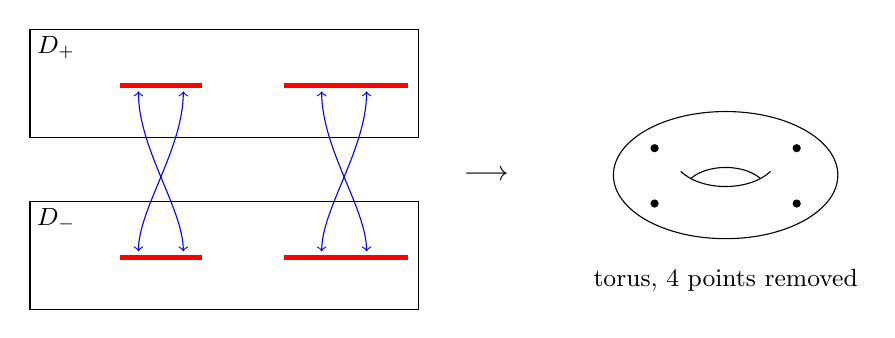
\begin{tikzpicture}[scale=0.95]
	% sheet +
	\begin{scope}
	\draw[thin] (-2.6,-0.6) rectangle (2.6,0.85);
	\node at (-2.25,0.6) {\small $D_+$};
	\draw[ultra thick, color=red] (-1.4,0.1) -- (-0.3,0.1);
	\draw[ultra thick, color=red] (0.8,0.1) -- (2.45,0.1);
	\end{scope}
	% sheet -
	\begin{scope}[yshift=-2.3cm]
	\draw[thin] (-2.6,-0.6) rectangle (2.6,0.85);
	\node at (-2.25,0.6) {\small $D_-$};
	\draw[ultra thick, color=red] (-1.4,0.1) -- (-0.3,0.1);
	\draw[ultra thick, color=red] (0.8,0.1) -- (2.45,0.1);
	\end{scope}
	% gluing arrows: each cut in D_+ is joined crosswise to the same cut in D_-
	\foreach \c in {-0.85, 1.6} {
		\draw[<->, thin, color=blue] ({\c-0.3},0.02) .. controls ({\c-0.3},-0.75) and ({\c+0.3},-1.55) .. ({\c+0.3},-2.12);
		\draw[<->, thin, color=blue] ({\c+0.3},0.02) .. controls ({\c+0.3},-0.75) and ({\c-0.3},-1.55) .. ({\c-0.3},-2.12);
	}
	% result
	\node at (3.5,-1.1) {$\longrightarrow$};
	\begin{scope}[xshift=6.7cm, yshift=-1.1cm]
		\draw[thin] (0,0) ellipse (1.5 and 0.85);
		\draw[thin] (-0.6,0.05) .. controls (-0.32,-0.22) and (0.32,-0.22) .. (0.6,0.05);
		\draw[thin] (-0.46,-0.04) .. controls (-0.23,0.15) and (0.23,0.15) .. (0.46,-0.04);
		\fill (-0.95,0.36) circle (0.055);
		\fill (0.95,0.36) circle (0.055);
		\fill (-0.95,-0.38) circle (0.055);
		\fill (0.95,-0.38) circle (0.055);
		\node at (0,-1.4) {\small torus, $4$ points removed};
	\end{scope}
\end{tikzpicture}
\end{center}

Each $D_\pm$ is a cylinder; gluing two cylinders along two pairs of slits produces a torus
with the four points $0, \pm 1, \infty$ removed. (Think of each cylinder as a sphere with
two slits; gluing crosswise along two slits is exactly the standard construction of a
genus-$1$ surface from two spheres with two handles' worth of identification.) We shall
verify this by computation in Section \ref{sec:RH}, and the reader should not feel obliged
to believe the picture until then.

Call the resulting Riemann surface $R$. The two branches assemble into a holomorphic
$g : R \to \C$, and the two inclusions $D_\pm \hookrightarrow \C\setminus\{0,\pm1\}$
assemble into a holomorphic covering map $\pi : R \to \C\setminus\{0,\pm 1\}$, with
$$
g(p)^2 = \pi(p)^3 - \pi(p) \qquad \text{for all } p \in R.
$$

\subsection{Compactifying the Cubic}\label{subsec:compactifycubic}

The surface $R$ above is missing four points. To restore them, we use the graph
description. Let
$$
R_1 = \{(z,w) \in \C^2 : w^2 = z^3 - z\}.
$$
One checks (this is an example sheet exercise, and we shall do the general case in Section
\ref{subsec:algebraic}) that $R_1$ is a Riemann surface: away from $w=0$ the projection
$(z,w)\mapsto z$ is a chart, and at the three points $(0,0),(\pm 1, 0)$ the projection
$(z,w)\mapsto w$ is a chart. It contains $R$ as the complement of those three points, so
$R_1$ restores $0$ and $\pm 1$. Only $\infty$ is missing.

To add it, change coordinates so that $\infty$ becomes finite. Put
$$
u = \frac{1}{z}, \qquad v = \frac{z}{w},
$$
so that $z = 1/u$ and $w = z/v = 1/(uv)$. Substituting into $w^2 = z^3 - z$:
$$
\frac{1}{u^2v^2} = \frac{1}{u^3} - \frac1u \implies u = v^2(1 - u^2).
$$
So set
$$
R_2 = \{(u,v)\in\C^2 : u = v^2(1-u^2)\},
$$
again a Riemann surface by the same argument, and note that $(u,v) = (0,0)$ lies on it --
this is our point at infinity. The map
$$
\Phi(z,w) = \left(\tfrac1z, \tfrac zw\right)
$$
is a conformal equivalence from $R_1 \setminus \{(0,0),(\pm1,0)\}$ onto
$R_2 \setminus \{(0,0)\}$, with inverse $(u,v)\mapsto (1/u, 1/(uv))$. Define
$$
\hat R = R_1 \cup_\Phi R_2.
$$

\begin{proposition}
	$\hat R$ is a compact Riemann surface.
\end{proposition}

\begin{proof}
	By Proposition \ref{prop:gluingsurfaces} we need only Hausdorffness and compactness.
	Define $\hat\pi : \hat R \to \Cinf$ by $\hat\pi(i_1(z,w)) = z$ and
	$\hat\pi(i_2(u,v)) = 1/u$; these agree on the overlap by construction of $\Phi$, so
	$\hat\pi$ is a well-defined continuous map, and it is holomorphic in the glued
	structure.

	\emph{Hausdorff.} Points both in $i_1(R_1)$, or both in $i_2(R_2)$, are separated
	there. The only points not in $i_2(R_2)$ are $i_1(0,0), i_1(\pm1,0)$, and the only
	point not in $i_1(R_1)$ is $i_2(0,0)$. These are separated by
	$\hat\pi^{-1}(D(0,2))$ and $\hat\pi^{-1}(\Cinf\setminus \overline D(0,2))$.

	\emph{Compact.} We show sequential compactness (which suffices, $\hat R$ being
	second countable and metrisable, or directly by a covering argument). Let $(p_n)$ be a
	sequence in $\hat R$. If some subsequence has $|\hat\pi(p_n)| \leq M$, pass to a further
	subsequence with $\hat\pi(p_n) \to z_0 \in \C$; there are at most two $w_0$ with
	$w_0^2 = h(z_0)$, so a further subsequence converges to some $i_1(z_0,w_0)$. Otherwise
	$|\hat\pi(p_n)|\to\infty$, and since $i_2(0,0)$ is the unique point with
	$\hat\pi = \infty$, and $\hat\pi$ is a proper map near there, $p_n \to i_2(0,0)$.
\end{proof}

We have obtained a compact Riemann surface $\hat R$ carrying a meromorphic function
$\hat\pi$ (of degree $2$, as we shall see) and a meromorphic $\hat g$ extending $g$, with
$\hat g^2 = \hat\pi^3 - \hat\pi$. This is the \vocab{elliptic curve} $w^2 = z^3 - z$, and
in Section \ref{sec:elliptic} we shall discover that it is conformally a complex torus.

\section{Branching and the Degree}\label{sec:branching}

The map $\hat p_k : \Cinf \to \Cinf$, $z \mapsto z^k$, is $k$-to-one except over $0$ and
$\infty$, where the $k$ preimages collide. This is the only local phenomenon there is: we
now prove that \emph{every} non-constant holomorphic map looks like $z \mapsto z^n$ in
suitable coordinates.

\subsection{The Local Normal Form}

\begin{proposition}[Local Normal Form]\label{prop:localform}
	Let $f : R \to S$ be a non-constant holomorphic map of Riemann surfaces and $p \in R$.
	Then there is an integer $n \geq 1$ and charts $(\phi, U)$ about $p$ and $(\psi, V)$
	about $f(p)$ with $\phi(p) = 0$, $\psi(f(p)) = 0$ and
	$$
	\psi \circ f \circ \phi^{-1}(z) = z^n
	$$
	on $\phi(U)$.
\end{proposition}

\begin{proof}
	Start with any charts $(\phi_0, U_0)$ about $p$ and $(\psi, V)$ about $f(p)$,
	normalised so that $\phi_0(p) = 0$ and $\psi(f(p)) = 0$, with $f(U_0) \subseteq V$. The
	local expression $F = \psi \circ f \circ \phi_0^{-1}$ is holomorphic near $0$ with
	$F(0) = 0$, and is not identically zero by Corollary \ref{cor:notlocallyconstant}. So by
	Proposition \ref{prop:isolatedzeros} there is $n \geq 1$ and a holomorphic $G$ near $0$
	with
	$$
	F(z) = z^n G(z), \qquad G(0) \neq 0.
	$$
	Choose $\delta > 0$ with $D(0,\delta)$ inside the domain of $G$ and
	$G(D(0,\delta)) \subseteq D(G(0), |G(0)|)$; the latter disc misses $0$ and is
	simply connected, so there is a holomorphic branch $\rho$ of the $n$-th root on it.
	Put
	$$
	h(z) = z\,\rho(G(z)), \qquad z \in D(0,\delta),
	$$
	so that $h(z)^n = z^n G(z) = F(z)$. Now $h(0) = 0$ and
	$h'(0) = \rho(G(0)) \neq 0$, so by the inverse function theorem (Theorem \ref{thm:ift})
	$h$ is a biholomorphism from some $D(0,\varepsilon)$ onto an open set.

	Set $\phi = h \circ \phi_0$, restricted to $U = \phi_0^{-1}(D(0,\varepsilon))$. This is
	a chart (a composite of a chart with a biholomorphism) with $\phi(p) = 0$, and it is
	compatible with the existing structure since $h$ is biholomorphic. Finally
	\begin{align*}
	\psi \circ f \circ \phi^{-1}(z) &= \psi \circ f \circ \phi_0^{-1}\circ h^{-1}(z)\\
	&= F(h^{-1}(z)) = h(h^{-1}(z))^n = z^n. \qedhere
	\end{align*}
\end{proof}

\begin{definition}[Multiplicity]
	The integer $n$ of Proposition \ref{prop:localform} is the \vocab{multiplicity} (or
	\vocab{ramification index}, or \vocab{local degree}) of $f$ at $p$, written $\mult_f(p)$.
\end{definition}

\begin{lemma}
	$\mult_f(p)$ is well defined, i.e.\ independent of the charts chosen.
\end{lemma}

\begin{proof}
	If $z^n$ and $z^m$ are both local expressions, then they differ by pre-composition
	and post-composition with biholomorphisms fixing $0$. So $\alpha(z)^n = \beta(z^m)$ near
	$0$ with $\alpha,\beta$ biholomorphic and $\alpha(0)=\beta(0)=0$. Counting orders of
	vanishing at $0$: $\alpha$ and $\beta$ have simple zeros (their derivatives are
	non-zero), so the left side vanishes to order $n$ and the right to order $m$. Hence
	$n=m$.
\end{proof}

Equivalently: $\mult_f(p)$ is the order of the zero of $\psi\circ f\circ\phi^{-1} - \psi(f(p))$
at $\phi(p)$, in any charts.

\begin{definition}[Ramification and Branch Points]
	If $\mult_f(p) > 1$ we call $p$ a \vocab{ramification point} of $f$, and $f(p)$ a
	\vocab{branch point}. A point $q \in S$ with $f^{-1}(q)$ a single point $p$ of
	multiplicity $\deg f$ is \vocab{totally ramified}.
\end{definition}

The local picture is worth having firmly in mind. Under $z \mapsto z^n$, the disc
$|z|<\varepsilon$ is wrapped $n$ times around the disc $|w| < \varepsilon^n$: each of the
$n$ sectors of angle $2\pi/n$ is opened out to a full disc, and the $n$ preimages of a
point $w \neq 0$ merge into the single preimage $0$ of $0$.

\begin{center}
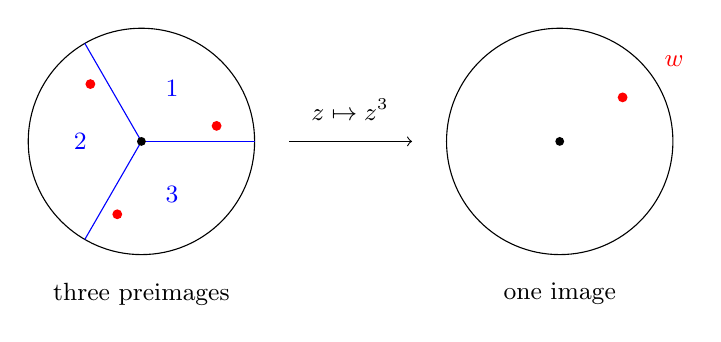
\begin{tikzpicture}[scale=1.25]
	% source disc with sectors
	\draw[thin] (0,0) circle (1.15);
	\foreach \a in {0,120,240} { \draw[thin, color=blue] (0,0) -- (\a:1.15); }
	\fill (0,0) circle (0.045);
	\foreach \a/\lab in {60/1, 180/2, 300/3} { \node[color=blue] at (\a:0.62) {\small $\lab$}; }
	\node at (0,-1.55) {\small three preimages};
	% the three cube roots of the point w below, one in each sector
	\foreach \a in {11.67,131.67,251.67} { \fill[color=red] (\a:0.78) circle (0.05); }
	% arrow
	\draw[->, thin] (1.5,0) -- (2.75,0);
	\node at (2.12,0.32) {\small $z \mapsto z^3$};
	% target disc
	\begin{scope}[xshift=4.25cm]
		\draw[thin] (0,0) circle (1.15);
		\fill (0,0) circle (0.045);
		\fill[color=red] (35:0.78) circle (0.05);
		\node[color=red] at (35:1.42) {\small $w$};
		\node at (0,-1.55) {\small one image};
	\end{scope}
\end{tikzpicture}
\end{center}

\begin{example}\label{ex:polymult}
	Let $f : \Cinf \to \Cinf$ be a polynomial $f(z) = a_dz^d + \cdots + a_0$ with
	$a_d \neq 0$ and $d \geq 1$, extended by $f(\infty) = \infty$. Away from $\infty$, the
	local expression of $f$ is $f$ itself and $\mult_f(p)$ is the order of the zero of
	$f(z) - f(p)$ at $p$; so the ramification points in $\C$ are exactly the zeros of $f'$.
	At $\infty$, use the chart $w = 1/z$ upstairs and downstairs:
	$$
	\frac{1}{f(1/w)} = \frac{w^d}{a_d + a_{d-1}w+\cdots+a_0w^d},
	$$
	which vanishes to order $d$ at $w = 0$. So $\mult_f(\infty) = d$, and $\infty$ is
	totally ramified whenever $d \geq 2$.
\end{example}

\begin{remark}	More generally, if $f : R \to \C$ is holomorphic and $(\phi, U)$ is any chart about $p$
	with $F = f\circ\phi^{-1}$, then writing $F(z) - F(z_0) = (z-z_0)^m G(z)$ with
	$G(z_0)\ne 0$ and $m = \mult_f(p)$, we get
	$$
	F'(z) = (z-z_0)^{m-1}\left(mG(z) + (z-z_0)G'(z)\right),
	$$
	so $F'(z_0) = 0$ if and only if $m > 1$. The ramification points are the zeros of the
	derivative in any chart. Since $F'$ is not identically zero (as $f$ is non-constant),
	its zeros are isolated: \emph{a non-constant holomorphic map has a discrete set of
	ramification points}. If $R$ is compact, there are only finitely many.
\end{remark}

\begin{lemma}[Multiplicativity]\label{lem:multmult}
	If $f : R \to S$ and $g : S \to T$ are non-constant holomorphic, then
	$$
	\mult_{g\circ f}(p) = \mult_g(f(p))\cdot \mult_f(p).
	$$
\end{lemma}

\begin{proof}
	Choose charts in which $f$ is $z \mapsto z^{m}$ with $m = \mult_f(p)$, and in which $g$
	is $w \mapsto w^{n}$ with $n = \mult_g(f(p))$; we may take the target chart for $f$ to
	be the source chart for $g$, since both are just `some chart about $f(p)$ sending it to
	$0$', and the local normal form allows us to choose the source chart freely at each
	stage --- more carefully, take the normal form charts for $g$ first, then run the proof
	of Proposition \ref{prop:localform} for $f$ with that target chart. Then $g\circ f$ has
	local expression $z \mapsto (z^{m})^{n} = z^{mn}$.
\end{proof}

\subsection{Proper Maps and the Degree}

\begin{definition}[Proper Map]
	A continuous map $f : R \to S$ is \vocab{proper} if $f^{-1}(K)$ is compact for every
	compact $K \subseteq S$.
\end{definition}

If $R$ is compact then every continuous $f : R \to S$ is proper, since a closed subset of
a compact space is compact. That is the case we shall use most often, but properness is
the right hypothesis in general: it is what makes fibres finite, and what stops points of
a fibre escaping to infinity as we move around in $S$.

\begin{example}\
	\begin{enumerate}[label=(\roman*)]
		\item A non-constant polynomial $f : \C \to \C$ is proper, since $|f(z)|\to\infty$
		as $|z|\to\infty$ and so the preimage of a bounded set is bounded and closed.
		\item $p_k : \Cs \to \Cs$ is proper: $|z^k| \to \infty$ as $|z| \to \infty$ and
		$|z^k|\to 0$ as $z \to 0$, so preimages of compact subsets of $\Cs$ stay away from
		both ends.
		\item \emph{(Non-examples.)} $\exp : \C \to \Cs$ is not proper, since
		$\exp^{-1}(\{1\}) = 2\pi i \Z$ is an infinite discrete set. The inclusion
		$\disc \hookrightarrow \C$ is not proper either, as $\overline{D}(0,1)$ has
		non-compact preimage $\disc$. Neither map has a sensible degree: $\exp$ is
		$\infty$-to-one, and the inclusion is one-to-one over $\disc$ and zero-to-one
		outside it.
	\end{enumerate}
\end{example}

The two properties of proper maps we need are the following.

\begin{lemma}\label{lem:properclosed}
	Let $f : R \to S$ be a proper continuous map of Riemann surfaces. Then $f$ is a closed
	map. If moreover $f$ is holomorphic and non-constant, every fibre $f^{-1}(q)$ is finite.
\end{lemma}

\begin{proof}
	For the fibres, $f^{-1}(q)$ is compact, being the preimage of the compact set $\{q\}$,
	and discrete by Corollary \ref{cor:notlocallyconstant}; a compact discrete space is
	finite.

	For closedness, let $A \subseteq R$ be closed and $q \in \overline{f(A)}$. Pick a chart
	$(\psi, V)$ about $q$ with $\psi(q) = 0$ and put
	$N = \psi^{-1}(\overline{D}(0,r))$ for some small $r > 0$ with
	$\overline{D}(0,r)\subseteq\psi(V)$, a compact neighbourhood of $q$. Then $f^{-1}(N)$
	is compact by properness, so $A \cap f^{-1}(N)$ is compact, and therefore
	$f\left(A \cap f^{-1}(N)\right)$ is compact and hence closed in the Hausdorff space $S$.
	Every neighbourhood of $q$ contained in the interior of $N$ meets $f(A)$, and the points
	of $f(A)$ it meets lie in $f(A\cap f^{-1}(N))$; so $q$ is in the closure of that set,
	which is the set itself. Hence $q \in f(A)$, and $f(A)$ is closed.
\end{proof}

\begin{theorem}[Valency Theorem]\label{thm:valency}
	Let $f : R \to S$ be a non-constant proper holomorphic map of Riemann surfaces. Then
	the function
	$$
	n(q) = \sum_{p \in f^{-1}(q)} \mult_f(p)
	$$
	is constant on $S$. In particular this applies to any non-constant holomorphic map of
	compact Riemann surfaces.
\end{theorem}

\begin{proof}
	First, each fibre $f^{-1}(q)$ is finite by Lemma \ref{lem:properclosed}, so $n$ is well
	defined and $\N$-valued. Since $S$ is connected it suffices to prove $n$ is locally
	constant.

	Fix $q_0 \in S$ and write $f^{-1}(q_0) = \{p_1, \dots, p_k\}$ with
	$m_i = \mult_f(p_i)$. Choose a chart $(\psi, V)$ about $q_0$ with $\psi(q_0) = 0$, and
	by Proposition \ref{prop:localform} charts $(\phi_i, U_i)$ about $p_i$ with
	$\psi f\phi_i^{-1}(z) = z^{m_i}$; shrinking, we may take the $U_i$ pairwise disjoint and
	contained in $f^{-1}(V)$.

	Let $U = \bigcup_i U_i$. Then $R \setminus U$ is closed in $R$, so
	$K = f(R\setminus U)$ is closed in $S$ by Lemma \ref{lem:properclosed}. Note that
	$q_0 \notin K$, since the whole fibre over $q_0$ lies in $U$. Put
	$$
	V' = V \setminus K,
	$$
	an open neighbourhood of $q_0$, and $U_i' = U_i \cap f^{-1}(V')$. Then
	$$
	f^{-1}(V') \subseteq U, \qquad \text{so} \qquad f^{-1}(V') = \coprod_{i=1}^k U_i'.
	$$
	On $U_i'$, in the charts $\phi_i$ and $\psi$, $f$ is the map $z \mapsto z^{m_i}$
	restricted to an open set; such a map takes each value $w \neq 0$ exactly $m_i$ times
	(counted without multiplicity, all multiplicities being $1$) and the value $0$ once with
	multiplicity $m_i$. Hence for every $q \in V'$,
	$$
	n(q) = \sum_{i=1}^{k}\ \sum_{p\in U_i' \cap f^{-1}(q)}\mult_f(p) = \sum_{i=1}^k m_i = n(q_0).
	$$
	So $n$ is constant on $V'$.
\end{proof}

\begin{definition}[Degree]
	The constant value $n$ of Theorem \ref{thm:valency} is the \vocab{degree} of $f$,
	written $\deg f$.
\end{definition}

Thus a non-constant proper holomorphic map is `$\deg f$-to-one, when points are counted
with multiplicity'; in particular this is true of any non-constant holomorphic map of
compact Riemann surfaces, which is the situation we shall almost always be in. Note that
$p_k : \Cs\to\Cs$ has degree $k$ and a polynomial $\C\to\C$ has degree equal to its degree
as a polynomial, so the notion is consistent with the classical one even off compact
surfaces.

\begin{corollary}\label{cor:degree1}
	A holomorphic map $f : R \to S$ of compact Riemann surfaces with $\deg f = 1$ is a
	conformal equivalence. In particular a holomorphic bijection of compact Riemann surfaces
	is a conformal equivalence.
\end{corollary}

\begin{proof}
	If $\deg f = 1$ then every fibre is a single point of multiplicity $1$, so $f$ is a
	bijection with no ramification points. By Proposition \ref{prop:localform} $f$ is
	locally biholomorphic, so $f^{-1}$ is holomorphic.
\end{proof}

\begin{example}
	If $f$ is a polynomial of degree $d$, regarded as $f : \Cinf\to\Cinf$, then $\deg f = d$:
	compute $n(\infty)$, which by Example \ref{ex:polymult} is $\mult_f(\infty) = d$ since
	$\infty$ is the only preimage of $\infty$.
\end{example}

\begin{corollary}[Fundamental Theorem of Algebra]
	A polynomial $f \in \C[z]$ of degree $d \geq 1$ has exactly $d$ roots in $\C$, counted
	with multiplicity.
\end{corollary}

\begin{proof}
	Extend to $f: \Cinf\to\Cinf$, of degree $d$. Then $n(0) = d$, and $f^{-1}(0) \subseteq \C$
	since $f(\infty)=\infty$. The multiplicity of $f$ at a root is the order of the root.
\end{proof}

\begin{example}
	A rational function $f = p/q$ in lowest terms with $\deg p = m$, $\deg q = n$ has
	$\deg f = \max(m,n)$ as a map $\Cinf\to\Cinf$. Indeed if $m > n$ then $\infty$ is the
	only preimage of $\infty$ with multiplicity $m - n$... rather than pursue this, compute
	$n(w)$ for generic $w$: the equation $p(z) - wq(z) = 0$ has $\max(m,n)$ roots for all
	but finitely many $w$, since the leading coefficient of $p - wq$ vanishes for at most
	one $w$.
\end{example}

\begin{example}[The Two-Sheeted Cover of the Sphere]\label{ex:2sheeted}
	Consider $\hat p_2 : \Cinf\to\Cinf$, $z\mapsto z^2$. It has degree $2$, and its
	branch points are $0$ and $\infty$, each totally ramified. Topologically: take two
	copies of the sphere, slit each along an arc from $0$ to $\infty$, and glue crosswise.
	The result is again a sphere.
\end{example}

\begin{center}
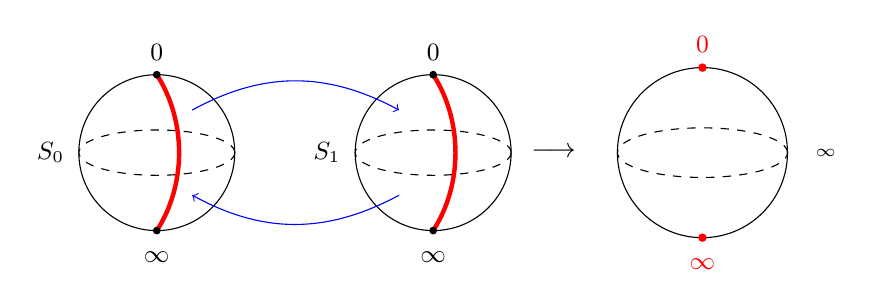
\begin{tikzpicture}[scale=0.9]
	% two slit spheres side by side
	\foreach \s/\x/\lab in {0/0/{S_0}, 1/3.9/{S_1}} {
	\begin{scope}[xshift={\x cm}]
		\draw[thin] (0,0) circle (1.1);
		\draw[thin, dashed] (0,0) ellipse (1.1 and 0.32);
		\draw[ultra thick, color=red] (0,1.1) .. controls (0.42,0.45) and (0.42,-0.45) .. (0,-1.1);
		\fill (0,1.1) circle (0.055);
		\fill (0,-1.1) circle (0.055);
		\node at (0,1.42) {\small $0$};
		\node at (0,-1.48) {\small $\infty$};
		\node at (-1.5,0) {\small $\lab$};
	\end{scope}}
	% crosswise gluing arrows
	\draw[->, thin, color=blue] (0.5,0.6) .. controls (1.5,1.15) and (2.4,1.15) .. (3.42,0.6);
	\draw[->, thin, color=blue] (3.42,-0.6) .. controls (2.4,-1.15) and (1.5,-1.15) .. (0.5,-0.6);
	\node at (5.6,0) {$\longrightarrow$};
	% resulting sphere
	\begin{scope}[xshift=7.7cm]
		\draw[thin] (0,0) circle (1.2);
		\draw[thin, dashed] (0,0) ellipse (1.2 and 0.35);
		\fill[color=red] (0,1.2) circle (0.06);
		\fill[color=red] (0,-1.2) circle (0.06);
		\node[color=red] at (0,1.52) {\small $0$};
		\node[color=red] at (0,-1.58) {\small $\infty$};
		\node at (1.75,0) {\small $\Cinf$};
	\end{scope}
\end{tikzpicture}
\end{center}

Gluing the upper side of the slit in $S_0$ to the lower side of the slit in $S_1$, and
vice versa, returns a sphere; the two red points are the branch points $0$ and $\infty$,
and over every other point there are two preimages. That the total space is again a
sphere and not, say, a torus is
a genuine constraint, and Riemann--Hurwitz is the tool that makes such constraints
computable.

\subsection{Riemann Surfaces of Algebraic Functions}\label{subsec:algebraic}

The examples $w^2 = z^3 - z$ and $w^k = z$ are instances of a general construction. Let
$$
P(z,w) = w^d + c_{d-1}(z)w^{d-1} + \cdots + c_0(z)
$$
be a polynomial in $w$ whose coefficients are polynomials in $z$, and suppose $P$ is
irreducible in $\C[z,w]$. The \vocab{algebraic function} $w(z)$ defined by $P(z,w)=0$ is
the classical object; the modern one is the surface
$$
X' = \{(z,w) \in \C^2 : P(z,w) = 0\}.
$$

\begin{proposition}\label{prop:algebraicsurface}
	Suppose $X'$ is \vocab{smooth}, that is, at every point of $X'$ at least one of
	$\partial P/\partial z$, $\partial P /\partial w$ is non-zero. Then $X'$ is a Riemann
	surface, with charts given by the coordinate projections, and
	$\pi_z : X' \to \C$, $(z,w)\mapsto z$, is holomorphic.
\end{proposition}

\begin{proof}[Proof sketch]
	$X'$ is Hausdorff and second countable as a subspace of $\C^2$. Near a point
	$(z_0,w_0)$ with $\partial P/\partial w \neq 0$, the holomorphic implicit function
	theorem provides a holomorphic $\eta$ near $z_0$ with $\eta(z_0)=w_0$ and
	$P(z,\eta(z))=0$, and the graph of $\eta$ is a neighbourhood of $(z_0,w_0)$ in $X'$; so
	$\pi_z$ is a homeomorphism there and serves as a chart. Symmetrically, where
	$\partial P/\partial z \neq 0$, $\pi_w$ is a chart. Smoothness says these cover $X'$.
	The transition functions are $\eta$ and its inverse, which are holomorphic. Connectedness
	is the one genuinely non-trivial point, and it follows from irreducibility of $P$; we
	verify it by hand in the examples we need.
\end{proof}

Away from the finitely many $z$ for which $P(z,\cdot)$ has a repeated root -- the
\vocab{discriminant locus} -- the map $\pi_z$ is a $d$-sheeted covering map, since the $d$
roots $w$ vary holomorphically and distinctly. Over the discriminant locus, roots collide
and $\pi_z$ ramifies. Compactifying (by gluing in charts at $\infty$, as in Section
\ref{subsec:compactifycubic}) gives a compact Riemann surface $X$ with a degree-$d$
meromorphic function $\hat\pi_z : X \to \Cinf$.

\begin{example}[Fermat Curves]\label{ex:fermat}
	Let $d \geq 1$ and
	$$
	F_d' = \{(x,y)\in\C^2 : x^d + y^d = 1\}.
	$$
	Here $P = y^d + x^d - 1$, with $\partial P/\partial y = dy^{d-1}$ and
	$\partial P /\partial x = dx^{d-1}$, which vanish simultaneously only at $(0,0)$, not a
	point of $F_d'$. So $F_d'$ is smooth.

	Concretely, $\pi_x$ has local inverse $x \mapsto (x, \sqrt[d]{1-x^d})$, which exists
	and is holomorphic near any $x_0$ with $x_0^d \neq 1$, i.e.\ away from
	$y_0 = 0$; and $\pi_y$ provides charts near the points where $y = 0$, since there
	$x \ne 0$. These cover $F_d'$.

	For connectedness: let
	$$
	D = \C\setminus\bigcup_{i=0}^{d-1}\{t\zeta_d^i : t \geq 1\}, \qquad \zeta_d = e^{2\pi i/d},
	$$
	the plane with $d$ radial slits removed. This is simply connected and $1 - x^d$ does not
	vanish on it, so there are $d$ holomorphic branches of $(1-x^d)^{1/d}$ on $D$, each
	extending continuously to the slit endpoints $\zeta_d^i$. Given $(x_0,y_0)\in F_d'$ with
	$x_0\in D$, choose the branch $y$ with $y(x_0)=y_0$ and a path $\gamma$ in $D$ from
	$x_0$ to $1$; then $t\mapsto (\gamma(t), y(\gamma(t)))$ joins $(x_0,y_0)$ to $(1,0)$.
	Points with $x_0 \notin D$ can first be joined to nearby points with $x_0 \in D$, as $D$
	is dense. So $F_d'$ is path-connected, hence a Riemann surface.

	The compactification $F_d$ is obtained by gluing on a second chart at infinity (an
	example sheet exercise), and $\hat\pi_x : F_d \to \Cinf$ has degree $d$. Its
	ramification points are the $d$ points $(\zeta_d^i, 0)$, each of multiplicity $d$ (there
	$1 - x^d$ has a simple zero, so $y = (1-x^d)^{1/d}$ is a $d$-th root of a simple zero),
	and $\hat\pi_x^{-1}(\infty)$ consists of $d$ distinct unramified points. We compute the
	genus of $F_d$ in Example \ref{ex:fermatgenus}.
\end{example}

\section{Euler Characteristic and Riemann--Hurwitz}\label{sec:RH}

Everything so far has been local or analytic. We now bring in topology, and the payoff is
immediate: the degree and ramification of a holomorphic map determine the topology of its
source from that of its target.

\subsection{Triangulations and the Euler Characteristic}

\begin{definition}[Triangulation]
	Let $S$ be a compact Riemann surface. A \vocab{topological triangle} in $S$ is a
	continuous embedding $\Delta \hookrightarrow S$ of a closed non-degenerate triangle
	$\Delta \subseteq \R^2$. A \vocab{triangulation} of $S$ is a finite collection
	$\{\Delta_i\}$ of topological triangles such that
	\begin{enumerate}[label=(\roman*)]
		\item $\bigcup_i \Delta_i = S$;
		\item for $i \neq j$, $\Delta_i \cap \Delta_j$ is empty, a common vertex, or a
		common edge;
		\item each edge lies in exactly two triangles.
	\end{enumerate}
\end{definition}

\begin{definition}[Euler Characteristic]
	The \vocab{Euler characteristic} of a triangulation is $\chi = V - E + F$, where $V, E,
	F$ count vertices, edges and faces.
\end{definition}

\begin{lemma}\label{lem:triangexists}
	Every compact Riemann surface admits a triangulation, and $\chi$ is independent of the
	triangulation chosen.
\end{lemma}

We take this on trust; the first part is Rad\'o's theorem and the second is the
topological invariance of simplicial homology, proved in II Algebraic Topology (where
$\chi = \sum_i (-1)^i \operatorname{rank} H_i$). We write $\chi(S)$ for the common value.

\begin{example}
	$\chi(\Cinf) = 2$. Triangulate the sphere as the boundary of a tetrahedron:
	$V - E + F = 4 - 6 + 4 = 2$.
\end{example}

\begin{example}
	$\chi(\C/\Lambda) = 0$. Represent the torus as a square with opposite sides identified
	and cut it into two triangles by a diagonal. After identification there is $V=1$ vertex,
	$E = 3$ edges (two sides and the diagonal), and $F = 2$ faces, giving
	$1 - 3 + 2 = 0$. (Strictly this is not a triangulation in the sense above, since the two
	triangles share more than one edge; subdividing repairs this without changing $\chi$.)
\end{example}

We quote from II Algebraic Topology the classification of surfaces: every compact
connected orientable surface is homeomorphic to $\Sigma_g$, the $g$-holed torus, for a
unique $g \geq 0$, and
$$
\chi(\Sigma_g) = 2 - 2g.
$$
A Riemann surface is orientable, since holomorphic transition functions have positive
Jacobian determinant $|\phi'|^2 > 0$. So a compact Riemann surface is homeomorphic to some
$\Sigma_g$, and $\chi$ determines it up to homeomorphism.

\begin{definition}[Genus]
	The \vocab{genus} of a compact Riemann surface $S$ is $g(S) = (2 - \chi(S))/2$.
\end{definition}

The standard picture of $\Sigma_g$ is a sphere with $g$ handles; equivalently it is a
$4g$-gon with its edges identified in the pattern
$a_1b_1a_1^{-1}b_1^{-1}\cdots a_gb_ga_g^{-1}b_g^{-1}$. For $g = 2$:

\begin{center}
\begin{tikzpicture}[scale=1]
	% genus 2 surface
	\begin{scope}
		\draw[thin] plot[smooth cycle, tension=0.75] coordinates
			{(-2.5,0) (-1.8,0.95) (-0.7,0.6) (0,0.85) (0.7,0.6) (1.8,0.95) (2.5,0)
			 (1.8,-0.95) (0.7,-0.6) (0,-0.85) (-0.7,-0.6) (-1.8,-0.95)};
		% holes, drawn in the standard two-arc way
		\foreach \c in {-1.25, 1.25} {
			\draw[thin] ({\c-0.44},0.06) .. controls ({\c-0.22},-0.16) and ({\c+0.22},-0.16) .. ({\c+0.44},0.06);
			\draw[thin] ({\c-0.33},-0.02) .. controls ({\c-0.17},0.12) and ({\c+0.17},0.12) .. ({\c+0.33},-0.02);
		}
	\end{scope}
	\node at (0,-1.55) {\small $\Sigma_2$};
	% octagon
	\begin{scope}[xshift=6.3cm]
		\foreach \i in {0,...,7} {
			\pgfmathsetmacro\a{22.5 + \i*45}
			\pgfmathsetmacro\b{22.5 + (\i+1)*45}
			\draw[thick] (\a:1.5) -- (\b:1.5);
		}
		\node at (45:1.72) {\small $a_1$};
		\node at (90:1.65) {\small $b_1$};
		\node at (135:1.78) {\small $a_1^{-1}$};
		\node at (180:1.88) {\small $b_1^{-1}$};
		\node at (225:1.78) {\small $a_2$};
		\node at (270:1.65) {\small $b_2$};
		\node at (315:1.78) {\small $a_2^{-1}$};
		\node at (0:1.88) {\small $b_2^{-1}$};
		\node at (0,-2.15) {\small the $8$-gon};
	\end{scope}
\end{tikzpicture}
\end{center}

From the octagon picture one reads off $\chi(\Sigma_2)$ directly: all $8$ vertices are
identified to one, the $8$ edges become $4$, and there is $1$ face, giving
$1 - 4 + 1 = -2 = 2 - 2\cdot 2$.

\subsection{The Riemann--Hurwitz Formula}

\begin{theorem}[Riemann--Hurwitz]\label{thm:RH}
	Let $f : R \to S$ be a non-constant holomorphic map of compact Riemann surfaces of
	degree $n$. Then
	$$
	\chi(R) = n\,\chi(S) - \sum_{p \in R}\left(\mult_f(p) - 1\right).
	$$
	Equivalently, in terms of genera,
	$$
	2g(R) - 2 = n\left(2g(S) - 2\right) + \sum_{p\in R}\left(\mult_f(p)-1\right).
	$$
\end{theorem}

The sum is finite: as we observed above, the ramification points of $f$ are isolated, and
$R$ is compact, so there are finitely many.

\begin{proof}
	As in the proof of the valency theorem, every $q \in S$ has an open neighbourhood $V_q$
	which is \vocab{well covered}: $f^{-1}(V_q)$ is a disjoint union of open sets on each of
	which $f$ is, in suitable charts, a power map $z \mapsto z^m$, and $V_q$ contains no
	branch point other than possibly $q$. By compactness of $S$, finitely many
	$V_{q_1},\dots,V_{q_r}$ cover $S$; in particular there are finitely many branch points.

	Choose a triangulation of $S$ and subdivide it repeatedly (barycentrically, say) until
	\begin{enumerate}[label=(\roman*)]
		\item every branch point of $f$ is a vertex, and
		\item every triangle is contained in some $V_{q_i}$.
	\end{enumerate}
	Both are achievable: (i) by first taking a triangulation with the finitely many branch
	points among the vertices, and (ii) since subdivision makes the triangles arbitrarily
	small and the $V_{q_i}$ have a Lebesgue number.

	Now pull back. If $\Delta \subseteq V_{q_i}$ is a (closed) triangle then
	$f^{-1}(\Delta)$ is a disjoint union of triangles, each mapped homeomorphically onto
	$\Delta$ by $f$; the same for edges. Indeed $\Delta$ is simply connected and, since its
	interior contains no branch point, $f$ restricted over the interior is a covering map of
	degree $n$; and the branch points on $\partial \Delta$ are vertices, where the local
	picture $z \mapsto z^m$ still sends the $m$ triangle-corners upstairs homeomorphically
	onto the corner downstairs. So the preimages of the triangles of $S$ form a
	triangulation of $R$, with
	$$
	F_R = n F_S, \qquad E_R = n E_S,
	$$
	since each face and each edge downstairs has exactly $n$ preimages.

	Vertices are where the count fails. For $q \in S$ a vertex, the valency theorem gives
	\begin{align*}
	\left|f^{-1}(q)\right| = \sum_{p \in f^{-1}(q)} 1
	&= \sum_{p\in f^{-1}(q)}\mult_f(p) - \sum_{p\in f^{-1}(q)}\left(\mult_f(p)-1\right)\\
	&= n - \sum_{p\in f^{-1}(q)}\left(\mult_f(p)-1\right).
	\end{align*}
	Summing over the vertices $q$ of $S$, and noting that every ramification point of $f$
	lies over a branch point, which is a vertex,
	$$
	V_R = nV_S - \sum_{p\in R}\left(\mult_f(p)-1\right).
	$$
	Therefore
	$$
	\chi(R) = V_R - E_R + F_R = n(V_S - E_S + F_S) - \sum_{p\in R}(\mult_f(p)-1),
	$$
	which is the first formula. The second follows by substituting $\chi = 2-2g$.
\end{proof}

\begin{center}
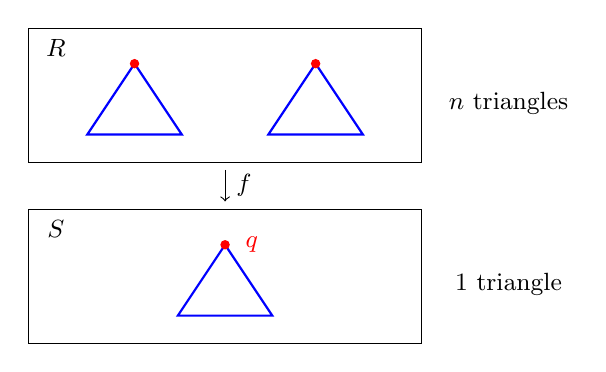
\begin{tikzpicture}[scale=1]
	% upstairs: two triangles over one
	\begin{scope}[yshift=2.3cm]
		\draw[thin] (-2.5,-0.75) rectangle (2.5,0.95);
		\node at (-2.15,0.7) {\small $R$};
		\draw[thick, color=blue] (-1.75,-0.4) -- (-0.55,-0.4) -- (-1.15,0.5) -- cycle;
		\draw[thick, color=blue] (0.55,-0.4) -- (1.75,-0.4) -- (1.15,0.5) -- cycle;
		\fill[color=red] (-1.15,0.5) circle (0.06);
		\fill[color=red] (1.15,0.5) circle (0.06);
	\end{scope}
	\draw[->, thin] (0,1.45) -- (0,1.05);
	\node at (0.24,1.25) {\small $f$};
	% downstairs
	\draw[thin] (-2.5,-0.75) rectangle (2.5,0.95);
	\node at (-2.15,0.7) {\small $S$};
	\draw[thick, color=blue] (-0.6,-0.4) -- (0.6,-0.4) -- (0,0.5) -- cycle;
	\fill[color=red] (0,0.5) circle (0.06);
	\node[color=red] at (0.34,0.5) {\small $q$};
	\node at (3.6,2.3) {\small $n$ triangles};
	\node at (3.6,0) {\small $1$ triangle};
\end{tikzpicture}
\end{center}

Each triangle and each edge downstairs has exactly $n$ preimages; only the vertices lying
under ramification points have fewer than $n$ preimages, and the deficiency is exactly
$\sum(\mult_f(p)-1)$.

\begin{remark}	The correction term $\sum_p (\mult_f(p)-1)$ is always even, being
	$\chi(R) - n\chi(S) = (2-2g(R)) - n(2 - 2g(S))$. This trivial-looking observation is
	surprisingly useful: it often pins down the ramification at a point we have not
	analysed.
\end{remark}

\subsection{First Applications}

\begin{corollary}\label{cor:unramified}
	Suppose $f : R \to S$ is an unramified non-constant holomorphic map of compact Riemann
	surfaces (equivalently, a covering map) of degree $n$. Then $g(R) - 1 = n(g(S)-1)$, and
	\begin{enumerate}[label=(\roman*)]
		\item if $g(S) = 0$ then $n = 1$ and $R \cong S \cong \Cinf$;
		\item if $g(S) = 1$ then $g(R) = 1$, and $n$ is unrestricted;
		\item if $g(S) \geq 2$ then either $n = 1$ and $f$ is a conformal equivalence, or
		$n \geq 2$ and $g(R) > g(S)$.
	\end{enumerate}
\end{corollary}

\begin{proof}
	Riemann--Hurwitz with no correction term gives $2g(R)-2 = n(2g(S)-2)$. If $g(S)=0$ then
	$g(R) - 1 = -n < 0$, forcing $g(R) = 0$ and $n = 1$; then $f$ is a conformal equivalence
	by Corollary \ref{cor:degree1}, and a genus $0$ compact surface is $\Cinf$ (which we
	prove in Corollary \ref{cor:genus0}). If $g(S)=1$ then $g(R)=1$ for any $n$. If
	$g(S)\geq 2$ then $g(R) - 1 = n(g(S)-1) \geq n$, so $n \geq 2$ gives
	$g(R) \geq 2g(S)-1 > g(S)$.
\end{proof}

\begin{example}
	That case (ii) is genuinely unrestricted: take $\Lambda_n = \genby{n, i}$ for
	$n \in \Z_{>0}$. Then $\Lambda_n \leq \Lambda_1 = \genby{1,i}$ with index $n$, so the
	identity on $\C$ descends to an unramified degree-$n$ map $\C/\Lambda_n \to \C/\Lambda_1$
	of tori.
\end{example}

\begin{example}[The Cubic Curve]\label{ex:cubicgenus}
	Let $\hat R$ be the compactification of the surface of $w^2 = z^3-z$ from Section
	\ref{subsec:compactifycubic}, with $\hat\pi : \hat R \to \Cinf$. Since a generic $z$
	has exactly two preimages $(z,\pm\sqrt{h(z)})$, $\deg\hat\pi = 2$. The branch points are
	$0, \pm 1$ (where $h$ has a simple zero, so the two sheets come together) and $\infty$;
	each is totally ramified, with a single preimage of multiplicity $2$. So
	$$
	2g(\hat R) - 2 = 2(0 - 2) + 4\cdot(2-1) = -4 + 4 = 0 \implies g(\hat R) = 1,
	$$
	confirming that $\hat R$ is a torus.
\end{example}

\begin{remark}
	Suppose we had not analysed the behaviour at $\infty$. Writing
	$$
	C = \sum_{p \in \hat\pi^{-1}(\infty)}\left(\mult_{\hat\pi}(p)-1\right),
	$$
	the correction term is
	$3 + C$, which must be even by the parity remark above; so $C$ is odd, and since
	$\deg\hat\pi = 2$ we must have $C = 1$, i.e.\ $\infty$ is a branch point. The parity
	argument has done the local analysis for us. This works whenever $\deg f = 2$.
\end{remark}

\begin{example}[Hyperelliptic Curves]
	More generally, let $h(z)$ be a polynomial of degree $d$ with $d$ distinct roots, and
	let $X$ be the compactification of $\{w^2 = h(z)\}$, with $\hat\pi : X \to \Cinf$ of
	degree $2$. The branch points in $\C$ are the $d$ roots of $h$. What happens at
	$\infty$? Setting $u = 1/z$, we get $w^2 = u^{-d}(1 + O(u))$, so $w \sim u^{-d/2}$: if
	$d$ is even there are two points over $\infty$, unramified; if $d$ is odd there is one,
	ramified. Either way the total correction is $d$ or $d+1$, i.e.\ $2\lceil d/2\rceil$,
	and
	$$
	2g(X) - 2 = 2(-2) + 2\left\lceil \tfrac d2\right\rceil \implies g(X) = \left\lceil \tfrac d2\right\rceil - 1 = \left\lfloor \frac{d-1}{2}\right\rfloor.
	$$
	So $d = 3, 4$ give genus $1$; $d = 5,6$ give genus $2$; and so on. These are the
	\vocab{hyperelliptic} curves.
\end{example}

\begin{example}[Fermat Curves and the Degree--Genus Formula]\label{ex:fermatgenus}
	Let $F_d$ be the compactified Fermat curve of Example \ref{ex:fermat}, with
	$\hat\pi_x : F_d \to \Cinf$ of degree $d$. There are $d$ ramification points
	$(\zeta_d^i, 0)$, each of multiplicity $d$, and no others. So
	$$
	2g(F_d) - 2 = d(0-2) + d(d-1) \implies g(F_d) = \frac{(d-1)(d-2)}{2}.
	$$

	This is an instance of the \vocab{degree--genus formula}: a smooth projective plane
	curve of degree $d$ has genus $(d-1)(d-2)/2$. For $d = 1, 2$ we get $g = 0$ (lines and
	conics are spheres); for $d = 3$, $g = 1$ (cubics are tori, as we found for
	$w^2 = z^3-z$ after homogenising); for $d = 4$, $g = 3$; and $g$ grows quadratically.
	In particular there exist compact Riemann surfaces of arbitrarily large genus --
	something not at all obvious from the definitions.

	Note that not every genus arises from a plane curve: $(d-1)(d-2)/2$ takes the values
	$0,0,1,3,6,10,\dots$, so no smooth plane curve has genus $2$. (Genus $2$ surfaces exist
	all the same -- they are hyperelliptic, by the previous example with $d = 5$.)
\end{example}

\section{Elliptic Functions and Complex Tori}\label{sec:elliptic}

We now describe all the meromorphic functions on the two compact surfaces we understand
best: the sphere, and the torus. The sphere is easy and classical. The torus is the heart
of the course, and the answer is remarkable -- every complex torus is a plane cubic curve,
and every elliptic function is a rational expression in one particular function and its
derivative.

\subsection{Meromorphic Functions on the Sphere}

\begin{proposition}\label{prop:rational}
	Every meromorphic function $f : \Cinf \to \Cinf$ is rational:
	$$
	f(z) = c\,\frac{(z-a_1)\cdots(z-a_m)}{(z-b_1)\cdots(z-b_n)}
	$$
	for some $c \in \Cs$ and $a_i, b_j \in \C$ with $a_i \neq b_j$.
\end{proposition}

\begin{proof}
	We may assume $f$ is non-constant. Replacing $f$ by $1/f$ if necessary (which does not
	affect the conclusion), assume $f(\infty)\neq\infty$. The poles of $f$ form a discrete
	closed subset of the compact space $\Cinf$, hence a finite set $\{b_1,\dots,b_{n'}\}$,
	and none is $\infty$. About each $b_j$ write the Laurent expansion
	$$
	f(z) = \sum_{l \geq -k_j} c_{j,l}(z-b_j)^l, \qquad c_{j,-k_j}\neq 0,
	$$
	and let $Q_j(z) = \sum_{l=-k_j}^{-1}c_{j,l}(z-b_j)^l$ be the principal part. Then
	$$
	g = f - \sum_{j=1}^{n'} Q_j
	$$
	is holomorphic on all of $\C$ -- the principal parts have cancelled every pole -- and
	is bounded near $\infty$, since $f$ is (having a finite value there) and each $Q_j \to 0$.
	By Liouville, $g$ is constant. So $f$ is a constant plus a sum of principal parts, which
	is a rational function.
\end{proof}

\begin{remark}
	If $f$ is written as above in lowest terms, its degree as a holomorphic map is
	$\max(m,n)$: this counts the preimages of a generic point. The zeros $a_i$ and poles
	$b_j$ may be prescribed arbitrarily, subject only to being finite in number -- there is
	no constraint on the sphere. On a torus we shall find that there is one.
\end{remark}

\subsection{Periodic Meromorphic Functions}

\begin{definition}[Period]
	Let $f : \C \to \Cinf$ be meromorphic. A \vocab{period} of $f$ is $\omega \in \C$ with
	$f(z+\omega) = f(z)$ for all $z$.
\end{definition}

The set $\Omega$ of periods is a subgroup of $(\C,+)$, and it is closed: if
$\omega_n \to \omega$ with $\omega_n \in \Omega$ then $f(z + \omega) = f(z)$ for all $z$
not a pole, by continuity, and hence everywhere.

\begin{lemma}\label{lem:periodgroups}
	Let $f$ be a non-constant meromorphic function on $\C$ with period group $\Omega$.
	Then exactly one of the following holds:
	\begin{enumerate}[label=(\roman*)]
		\item $\Omega = \{0\}$;
		\item $\Omega = \genby{\omega} \cong \Z$ for some $\omega \neq 0$;
		\item $\Omega = \genby{\omega_1,\omega_2} \cong \Z^2$ is a lattice, with
		$\omega_1/\omega_2 \notin \R$.
	\end{enumerate}
	(If $f$ is constant then $\Omega = \C$.)
\end{lemma}

\begin{proof}[Proof sketch]
	$\Omega$ is a closed subgroup of $\C \cong \R^2$, and the classification of such
	subgroups gives $\{0\}$, a discrete rank-$1$ or rank-$2$ subgroup, a line, a line plus a
	discrete complement, or all of $\C$. If $\Omega$ contained a line $\R\omega$ then the
	zeros of $f - f(z_0)$ would be non-discrete for suitable $z_0$, contradicting the
	identity theorem. The remaining possibilities are (i)--(iii). This is on the example
	sheets.
\end{proof}

\begin{definition}
	A non-constant meromorphic $f$ on $\C$ is \vocab{simply periodic} in case (ii), and
	\vocab{doubly periodic} or \vocab{elliptic} in case (iii).
\end{definition}

The reason to care is the correspondence with functions on quotients.

\begin{proposition}\label{prop:descend}
	Let $f$ be meromorphic on $\C$ and suppose $\Lambda \subseteq \Omega$ where
	$\Lambda \le \C$ is a lattice (respectively, $\genby{\omega} \subseteq \Omega$). Then
	there is a unique meromorphic function $\bar f$ on $\C/\Lambda$ (respectively on $\Cs$)
	with
	$$
	f = \bar f \circ \pi, \qquad \pi : \C \to \C/\Lambda \ \ (\text{resp. } z \mapsto e^{2\pi i z/\omega}).
	$$
\end{proposition}

\begin{proof}
	Uniqueness is clear as $\pi$ is surjective. For existence set $\bar f(\pi(z)) = f(z)$,
	which is well defined by periodicity. It is holomorphic as a map to $\Cinf$ because
	$\pi$ is a covering map with local holomorphic inverses: near any point,
	$\bar f = f \circ (\pi|_{\tilde U})^{-1}$.
\end{proof}

Thus simply periodic functions are the same thing as meromorphic functions on
$\Cs \cong \C/\genby{\omega}$, and elliptic functions with $\Lambda \subseteq \Omega$ are
the same thing as meromorphic functions on the complex torus $\C/\Lambda$. Everything we
know about compact surfaces now applies.

\begin{corollary}
	A holomorphic doubly periodic function on $\C$ is constant.
\end{corollary}

\begin{proof}
	It descends to a holomorphic function on the compact surface $\C/\Lambda$, which is
	constant by Corollary \ref{cor:noholofnsoncompact}.
\end{proof}

\begin{corollary}\label{cor:degatleast2}
	A non-constant elliptic function, viewed as $\bar f : \C/\Lambda \to \Cinf$, has
	$\deg \bar f \geq 2$.
\end{corollary}

\begin{proof}
	If $\deg\bar f = 1$ then $\bar f$ is a conformal equivalence $\C/\Lambda \to \Cinf$ by
	Corollary \ref{cor:degree1}, contradicting $\chi(\C/\Lambda) = 0 \neq 2 = \chi(\Cinf)$.
	(Equivalently: Riemann--Hurwitz would give $0 = 1\cdot(-2) + 0$.)
\end{proof}

It is worth also seeing the classical proof, which is where the theory came from.

\begin{proof}[Second proof of Corollary \ref{cor:degatleast2}]
	Choose $z_0$ so that no zero or pole of $f$ lies on the boundary of the period
	parallelogram $P = z_0 + \{s\omega_1 + t\omega_2 : s,t\in[0,1]\}$; this is possible as
	there are finitely many such points modulo $\Lambda$. The residue theorem gives
	$$
	\sum_{z \text{ pole in } P^\circ} \res_z(f) = \frac{1}{2\pi i}\oint_{\partial P} f(z)\dd z = 0,
	$$
	because the contributions of opposite sides of $P$ cancel: $f$ takes the same values on
	them and they are traversed in opposite directions. If $f$ had a single simple pole in
	$P$, its residue would be non-zero, contradiction. So $f$ has either no poles (hence is
	constant) or at least two poles counted with multiplicity.
\end{proof}

\subsection{The Weierstrass $\wp$-Function}

We need a non-constant elliptic function to exist at all. By the above the simplest
possible has a single double pole per period parallelogram, and this pins down the
definition.

\begin{definition}[Weierstrass $\wp$-function]
	Let $\Lambda \subseteq \C$ be a lattice. The \vocab{Weierstrass $\wp$-function} is
	$$
	\wp(z) = \wp_\Lambda(z) = \frac{1}{z^2} + \sum_{\omega \in \Lambda\setminus\{0\}}
	\left(\frac{1}{(z-\omega)^2} - \frac{1}{\omega^2}\right).
	$$
\end{definition}

The subtracted terms $1/\omega^2$ are there purely to make the series converge; without
them it diverges. To prove convergence we need a lemma on lattice sums.

\begin{lemma}\label{lem:latticesum}
	Let $\Lambda = \genby{\omega_1,\omega_2}$ be a lattice and $t \in \R$. Then
	$$
	\sum_{\omega\in\Lambda\setminus\{0\}}\frac{1}{|\omega|^t}
	$$
	converges if and only if $t > 2$.
\end{lemma}

\begin{proof}
	Consider $Q = \{(t_1,t_2)\in\R^2 : |t_1| + |t_2| = 1\}$, a compact set, and the
	continuous function $(t_1,t_2)\mapsto |t_1\omega_1 + t_2\omega_2|$ on it. It attains a
	maximum $M$ and a minimum $m$, and $m > 0$ since $\omega_1, \omega_2$ are linearly
	independent over $\R$ so the expression vanishes only at the origin, which is not in
	$Q$. Given $(k,l) \in \Z^2\setminus\{0\}$, apply this with
	$t_1 = k/(|k|+|l|)$, $t_2 = l/(|k|+|l|)$ to get
	$$
	m(|k|+|l|) \leq |k\omega_1 + l\omega_2| \leq M(|k|+|l|).
	$$
	So the sum in question is bounded above and below by positive multiples of
	$$
	\sum_{(k,l)\neq(0,0)}\frac{1}{(|k|+|l|)^t}.
	$$
	For each $n \geq 1$ there are exactly $4n$ pairs $(k,l)$ with $|k|+|l| = n$, so this
	equals
	$$
	\sum_{n\geq 1}\frac{4n}{n^t} = 4\sum_{n\geq1}\frac{1}{n^{t-1}},
	$$
	which converges if and only if $t - 1 > 1$.
\end{proof}

Notice that the same estimate shows every bounded region contains only finitely many
lattice points, which is what we assumed in Proposition \ref{prop:torusstructure}.

\begin{theorem}\label{thm:wp}
	$\wp_\Lambda$ is a well-defined elliptic function whose period group is exactly
	$\Lambda$. It is even, its poles are precisely the points of $\Lambda$, each a double
	pole, and $\deg\wp_\Lambda = 2$ as a map $\C/\Lambda\to\Cinf$.
\end{theorem}

\begin{proof}
	\emph{Convergence.} Fix $R > 0$ and work on $|z| \leq R$. For $\omega \neq 0$,
	$$
	\frac{1}{(z-\omega)^2}-\frac{1}{\omega^2} = \frac{\omega^2 - (z-\omega)^2}{\omega^2(z-\omega)^2}
	= \frac{z(2\omega - z)}{\omega^2(z-\omega)^2}
	= \frac{z}{\omega^2}\left(\frac{2}{z - \omega} + \frac{-z}{(z-\omega)^2}\right)\cdot(-1),
	$$
	so
	$$
	\left|\frac{1}{(z-\omega)^2}-\frac{1}{\omega^2}\right|
	\leq \frac{|z|}{|\omega|^2}\left(\frac{2}{|z-\omega|}+\frac{|z|}{|z-\omega|^2}\right).
	$$
	For all but finitely many $\omega$ we have $|\omega|\geq 2R$, whence
	$|z - \omega| \geq |\omega| - R \geq |\omega|/2 \geq R$, and the bound becomes
	$$
	\frac{R}{|\omega|^2}\left(\frac{4}{|\omega|}+\frac{R}{(|\omega|/2)\cdot R}\right)
	= \frac{R}{|\omega|^2}\cdot\frac{6}{|\omega|} = \frac{6R}{|\omega|^3}.
	$$
	By Lemma \ref{lem:latticesum} with $t = 3$, the series converges absolutely and
	uniformly on $|z|\leq R$ after discarding finitely many terms. So $\wp$ is a
	well-defined meromorphic function on $\C$, holomorphic away from $\Lambda$, with a
	double pole at each lattice point (the discarded terms contribute those).

	\emph{Evenness.} Replacing $z$ by $-z$ and $\omega$ by $-\omega$ permutes the terms of
	the (absolutely convergent) sum, so $\wp(-z)=\wp(z)$.

	\emph{Periodicity.} Differentiating term by term (legitimate by local uniform
	convergence),
	$$
	\wp'(z) = -2\sum_{\omega\in\Lambda}\frac{1}{(z-\omega)^3},
	$$
	which is manifestly $\Lambda$-periodic, since translating $z$ by $\omega_0 \in\Lambda$
	just permutes the summands. Fix $\omega_0 \in \Lambda$ and put
	$F(z) = \wp(z+\omega_0)-\wp(z)$. Then $F' = 0$, so $F$ is constant, say $F \equiv c$.
	Now take $z = -\omega_0/2$, which is not a pole if $\omega_0/2 \notin\Lambda$ (and if it
	is, replace $\omega_0$ by a generator and argue for generators, which suffices):
	$$
	c = \wp(\omega_0/2)-\wp(-\omega_0/2) = 0
	$$
	by evenness. So $\omega_0$ is a period, and $\Lambda \subseteq \Omega$.

	Conversely the poles of $\wp$ are exactly $\Lambda$; a period must permute the poles, so
	$\Omega \subseteq \Lambda$ (as $0$ is a pole, any $\omega \in \Omega$ satisfies
	$-\omega \in \Lambda$). Hence $\Omega = \Lambda$.

	\emph{Degree.} On $\C/\Lambda$, $\wp$ has a single pole, at $0$, of order $2$. So
	$\deg\wp = n(\infty) = 2$.
\end{proof}

\begin{remark}
	The properties
	\begin{enumerate}[label=(\roman*)]
		\item $\wp$ is meromorphic with period lattice $\Lambda$,
		\item the poles of $\wp$ are exactly $\Lambda$, and
		\item $\wp(z) - z^{-2}\to 0$ as $z \to 0$
	\end{enumerate}
	characterise $\wp$ uniquely: if $\tilde\wp$ also has them then $\wp - \tilde\wp$ is
	holomorphic and elliptic, hence constant, and the constant is $0$ by (iii).
\end{remark}

\subsection{Ramification of $\wp$}

Since $\deg\wp = 2$, Riemann--Hurwitz gives
$$
0 = 2\cdot(-2) + \sum_p(\mult_\wp(p)-1) \implies \sum_p(\mult_\wp(p)-1) = 4,
$$
so $\wp$ has exactly four ramification points, each of multiplicity $2$ (multiplicity
cannot exceed the degree). Let us find them.

One is $p = 0$: the pole is double, so $\mult_\wp(0)=2$. The others are the zeros of
$\wp'$, since ramification points are the zeros of the derivative in a chart. Now $\wp'$
is odd (differentiate $\wp(-z)=\wp(z)$),
elliptic with period lattice $\Lambda$, and has a triple pole at each lattice point, so
$\deg\wp' = 3$ on $\C/\Lambda$. For any $\omega\in\Lambda$,
$$
\wp'(\omega/2) = \wp'(\omega/2 - \omega) = \wp'(-\omega/2) = -\wp'(\omega/2),
$$
using periodicity and oddness; hence $\wp'(\omega/2) = 0$ whenever $\omega/2\notin\Lambda$.
Taking $\omega = \omega_1, \omega_2, \omega_1+\omega_2$ gives three distinct zeros in
$\C/\Lambda$, namely the three non-zero \vocab{half-periods}. Since $\deg \wp'=3$ there are
no others, and all three are simple.

\begin{center}
\begin{tikzpicture}[scale=1.5]
	% parallelogram
	\draw[thin, color=gray] (0,0) -- (1.7,0) -- (2.25,1.35) -- (0.55,1.35) -- cycle;
	% lattice corners
	\foreach \x/\y in {0/0, 1.7/0, 2.25/1.35, 0.55/1.35} { \fill (\x,\y) circle (0.06); }
	% half periods
	\fill[color=red] (0.85,0) circle (0.06);
	\fill[color=red] (0.275,0.675) circle (0.06);
	\fill[color=red] (1.125,0.675) circle (0.06);
	\node at (-0.22,-0.1) {\small $0$};
	\node[color=red] at (0.85,-0.34) {\small $\tfrac{\omega_1}{2}$};
	\node[color=red] at (-0.15,0.72) {\small $\tfrac{\omega_2}{2}$};
	\node[color=red] at (1.62,0.72) {\small $\tfrac{\omega_1+\omega_2}{2}$};
	\node at (1.88,-0.14) {\small $\omega_1$};
	\node at (0.4,1.52) {\small $\omega_2$};
\end{tikzpicture}
\end{center}

\begin{proposition}\label{prop:wpbranch}
	The four ramification points of $\wp : \C/\Lambda \to \Cinf$ are
	$0, \omega_1/2, \omega_2/2, (\omega_1+\omega_2)/2$, each of multiplicity $2$, and their
	images
	$$
	\infty, \quad e_1 = \wp(\omega_1/2), \quad e_2 = \wp(\omega_2/2), \quad e_3 = \wp\!\left(\tfrac{\omega_1+\omega_2}{2}\right)
	$$
	are four distinct points of $\Cinf$.
\end{proposition}

\begin{proof}
	We have found the four ramification points and know each has multiplicity $2$. They
	must have distinct images: if two of them mapped to the same $q$, then $n(q)$ would be
	at least $4 > 2 = \deg\wp$.
\end{proof}

So $\wp$ realises $\C/\Lambda$ as a two-sheeted cover of the sphere branched over four
points -- exactly the description of the surface of $w^2 = z^3-z$ found in Example
\ref{ex:cubicgenus}. This is not a coincidence.

\subsection{The Differential Equation}

\begin{proposition}\label{prop:wpode}
	There are constants $g_2, g_3 \in \C$, depending only on $\Lambda$, such that
	$$
	(\wp')^2 = 4\wp^3 - g_2\wp - g_3.
	$$
\end{proposition}

\begin{proof}
	Near $z = 0$ we expand. Since $\wp$ is even and $\wp(z) - z^{-2}$ vanishes at $0$, its
	Laurent series has the form
	$$
	\wp(z) = \frac{1}{z^2} + az^2 + bz^4 + O(z^6)
	$$
	(no odd powers, and no constant term). Cubing,
	$$
	\wp(z)^3 = \frac{1}{z^6} + \frac{3a}{z^2} + 3b + O(z^2),
	$$
	while differentiating and squaring,
	$$
	\wp'(z) = \frac{-2}{z^3}+2az+4bz^3+O(z^5), \qquad
	\wp'(z)^2 = \frac{4}{z^6} - \frac{8a}{z^2} - 16 b + O(z^2).
	$$
	Hence
	$$
	\wp'(z)^2 - 4\wp(z)^3 = -\frac{20a}{z^2} - 28b + O(z^2).
	$$
	Set $g_2 = 20a$. Then
	$$
	H := (\wp')^2 - 4\wp^3 + g_2\wp
	$$
	is elliptic, and near $0$ it equals $-28b + O(z^2) + g_2 \cdot O(z^2)$, so it is
	holomorphic at $0$. Its only possible poles were at $\Lambda$, so $H$ is a holomorphic
	elliptic function, hence constant; call the constant $-g_3$. Rearranging gives the
	result.
\end{proof}

\begin{remark}
	The constants are computable: expanding $\wp$ gives
	$g_2 = 60\sum_{\omega\neq0}\omega^{-4}$ and $g_3 = 140\sum_{\omega\neq0}\omega^{-6}$,
	which converge by Lemma \ref{lem:latticesum}. We shall not need this.
\end{remark}

\begin{corollary}\label{cor:eiroots}
	$e_1, e_2, e_3$ are the three roots of $4X^3 - g_2X - g_3$; they are distinct, and
	$e_1+e_2+e_3 = 0$. Moreover
	$$
	(\wp')^2 = 4(\wp - e_1)(\wp-e_2)(\wp-e_3).
	$$
\end{corollary}

\begin{proof}
	At $z = \omega_i/2$ we have $\wp'(z) = 0$ and $\wp(z) = e_i$, so
	$0 = 4e_i^3 - g_2e_i - g_3$. The $e_i$ are distinct by Proposition \ref{prop:wpbranch},
	so they are all three roots; the sum of the roots is $-(\text{coefficient of }X^2)/4 = 0$.
	The factorisation follows.
\end{proof}

\subsection{The Torus as a Cubic Curve}

\begin{theorem}\label{thm:toruscubic}
	Let $\Lambda\subseteq\C$ be a lattice with invariants $g_2, g_3$ as above, and let
	$$
	X' = \{(x,y)\in\C^2 : y^2 = 4x^3-g_2x-g_3\},
	$$
	with $X = X'\cup\{\infty\}$ its one-point compactification (a compact Riemann surface,
	as in Section \ref{subsec:compactifycubic}). Then
	$$
	\C/\Lambda \cong X
	$$
	as Riemann surfaces, via $z + \Lambda \mapsto (\wp(z),\wp'(z))$ and $0 \mapsto \infty$.
\end{theorem}

\begin{proof}
	Since $4X^3-g_2X-g_3 = 4(X-e_1)(X-e_2)(X-e_3)$ has distinct roots, $X'$ is smooth and
	is a Riemann surface with coordinate projections as charts (Proposition
	\ref{prop:algebraicsurface}), and $X$ is its compactification.

	Define $F : \C\setminus\Lambda \to X'$ by $F(z) = (\wp(z),\wp'(z))$. Its image lies in
	$X'$ by Proposition \ref{prop:wpode}. It is holomorphic: composed with the chart
	$\pi_x$ it is $\wp$, and composed with $\pi_y$ it is $\wp'$, both holomorphic. Extending
	by $F(\omega)=\infty$ for $\omega \in \Lambda$ gives a holomorphic map $\C \to X$ (the
	point $\infty$ of $X$ is exactly where both coordinates blow up, and the local
	computation there is as in Section \ref{subsec:compactifycubic}). Since $F$ is
	$\Lambda$-periodic it descends, by Proposition \ref{prop:descend}, to a holomorphic
	$$
	\Phi : \C/\Lambda \to X.
	$$

	$\Phi$ is non-constant, and $\C/\Lambda$ is compact, so $\Phi$ is surjective by
	Corollary \ref{cor:compactsurjective}. It remains to prove injectivity, for then
	$\deg\Phi = 1$ and Corollary \ref{cor:degree1} finishes the proof.

	Work in the centred period parallelogram $P$ with vertices $\pm(\omega_1\pm\omega_2)/2$,
	whose interior $P^\circ$ maps injectively to $\C/\Lambda$ and contains exactly one
	point of each class except for those on $\partial P$. Suppose $\Phi(z)=\Phi(z')$ for
	$z,z' \in P^\circ$. Then $\wp(z)=\wp(z')$; as $\wp$ is even of degree $2$, the fibre of
	$\wp$ over a non-branch value is $\{\pm z\}$, so $z' = \pm z$ (and if $z$ is one of the
	four ramification points then $z'=z$ directly). Also $\wp'(z)=\wp'(z')$; if $z'=-z$
	then, $\wp'$ being odd, $\wp'(z) = -\wp'(z)$, so $\wp'(z)=0$ and $z$ is a half-period.
	But the non-zero half-periods lie on $\partial P$ for this centred parallelogram, and
	$z = 0$ gives $z' = -z = z$. Either way $z=z'$. Hence $\Phi$ is injective on $P^\circ$
	and so on $\C/\Lambda$.
\end{proof}

So the two families of genus-$1$ surfaces we have met -- complex tori and compactified
plane cubics -- coincide. The map $\Phi$ is what makes the addition law on a cubic curve
comprehensible: it is transported from the group $\C/\Lambda$.

\subsection{The Field of Elliptic Functions}

\begin{theorem}\label{thm:ellipticfield}
	Let $f$ be an elliptic function with period lattice containing $\Lambda$, and write
	$\wp = \wp_\Lambda$. Then there are rational functions $Q_1, Q_2$ with
	$$
	f(z) = Q_1(\wp(z)) + Q_2(\wp(z))\,\wp'(z).
	$$
	If $f$ is even then $Q_2 = 0$.
\end{theorem}

\begin{proof}
	\emph{Case 1: $f$ even.} We first reduce to a convenient normalisation. The function $f$
	and $\wp$ each have finitely many branch points on the compact surface $\C/\Lambda$, so
	we may pick distinct $c, d\in\C$ which are not among the values of $f$ at its
	ramification points. Replacing $f$ by
	$$
	\frac{f - c}{f - d},
	$$
	which is $f$ composed with a M\"obius map, hence still even and elliptic, and from which
	$f$ can be recovered by the inverse M\"obius map, we may assume all the zeros and poles
	of $f$ are simple and occur away from the ramification points of $\wp$.

	Since $f$ is even, its zeros come in pairs $\pm a_i$ and its poles in pairs $\pm b_j$
	(modulo $\Lambda$), with $a_i \not\equiv \pm a_j$ for $i \neq j$ and similarly for the
	$b_j$; say the zeros are $\{\pm a_1,\dots,\pm a_m\}$ and the poles
	$\{\pm b_1,\dots,\pm b_n\}$. Consider
	$$
	g(z) = \frac{(\wp(z)-\wp(a_1))\cdots(\wp(z)-\wp(a_m))}{(\wp(z)-\wp(b_1))\cdots(\wp(z)-\wp(b_n))}.
	$$
	Each factor $\wp(z)-\wp(a_i)$ is elliptic of degree $2$ with zeros exactly $\pm a_i$
	(simple, as $a_i$ is not a ramification point of $\wp$) and a double pole at $0$. So $g$
	has exactly the same zeros and poles as $f$ away from $0$, and at $0$ the pole orders are
	$2n - 2m$ in $g$ and, by the valency theorem applied to $f$, also match. Hence $f/g$ is
	an elliptic function with no zeros and no poles, so it is holomorphic, hence constant.
	Therefore $f = \lambda g$ is a rational function of $\wp$.

	\emph{Case 2: $f$ odd.} Then $f/\wp'$ is even (as $\wp'$ is odd) and elliptic, so
	$f/\wp' = Q_2(\wp)$ by Case 1, giving $f = Q_2(\wp)\wp'$.

	\emph{General case.} Write
	$$
	f(z) = \frac{f(z)+f(-z)}{2} + \frac{f(z)-f(-z)}{2},
	$$
	a sum of an even and an odd elliptic function, and apply the two cases.
\end{proof}

In the language of fields: the field $\mathcal{M}(\C/\Lambda)$ of meromorphic functions on
the torus is $\C(\wp)[\wp']$, a degree-$2$ extension of the rational function field
$\C(\wp)$, with $\wp'$ satisfying the quadratic $(\wp')^2 = 4\wp^3-g_2\wp-g_3$. Compare
Proposition \ref{prop:rational}, which says $\mathcal{M}(\Cinf) = \C(z)$. In both cases
the meromorphic functions on a compact Riemann surface form a field of transcendence
degree $1$ over $\C$ -- this is true in general, and is the beginning of the dictionary
between compact Riemann surfaces and algebraic curves.

\section{Quotients and Uniformisation}

We finish by classifying all Riemann surfaces, at least in principle. The classification
is startlingly clean: there are only three simply connected Riemann surfaces, and every
other surface is a quotient of one of them.

\subsection{Quotients by Group Actions}

\begin{definition}
	Let a group $G$ act on a topological space $X$ by homeomorphisms. The action is
	\begin{enumerate}[label=(\roman*)]
		\item \vocab{properly discontinuous} if for every compact $K \subseteq X$ the set
		$\{g\in G : g(K)\cap K \neq\emptyset\}$ is finite;
		\item \vocab{free} if $\stab_G(x) = \{1\}$ for every $x \in X$.
	\end{enumerate}
\end{definition}

\begin{example}
	A lattice $\Lambda$ acts on $\C$ by translation. This action is free (a non-zero
	translation has no fixed point) and properly discontinuous (a compact $K$ is bounded,
	and only finitely many $\lambda\in\Lambda$ have $|\lambda| \le \operatorname{diam}K$).
\end{example}

\begin{lemma}\label{lem:quotientcover}
	Let $G$ act freely and properly discontinuously by homeomorphisms on a Riemann surface
	$R$. Then $G\backslash R$ is Hausdorff and the quotient map $\pi : R \to G\backslash R$
	is a regular covering map.
\end{lemma}

\begin{proof}
	First, $\pi$ is open, since $\pi^{-1}(\pi(U)) = \bigcup_{g} g(U)$.

	\emph{Hausdorff.} Let $p, q \in R$ with $\pi(p)\neq\pi(q)$. Choose open $U\ni p$,
	$V\ni q$ with compact closures, and set $K = \bar U\cup\bar V$, compact. Then
	$$
	\{g \in G : g(\bar U)\cap \bar V \neq \emptyset\} \subseteq \{g : g(K)\cap K \neq\emptyset\}
	$$
	is finite, say $\{g_1,\dots,g_k\}$. For each $i$ we have $g_i p \neq q$ (else
	$\pi(p)=\pi(q)$), so choose disjoint open $U_i \ni p$ and $V_i \ni g_i q$. Shrinking to
	$$
	U' = U \cap \bigcap_i U_i, \qquad V' = V\cap\bigcap_i g_i^{-1}(V_i),
	$$
	we get $g(U')\cap V' = \emptyset$ for every $g \in G$. Then $\pi(U')$ and $\pi(V')$ are
	disjoint open neighbourhoods.

	\emph{Covering.} Let $p \in R$ and choose open $U\ni p$ with $\bar U$ compact, so that
	$\{g : g(\bar U)\cap\bar U\neq\emptyset\} = \{1, g_1,\dots,g_k\}$ is finite. Freeness
	gives $g_ip\neq p$, so choose disjoint open $U_i\ni p$, $V_i \ni g_ip$, and set
	$$
	U' = U\cap\bigcap_i\left(U_i \cap g_i^{-1}(V_i)\right).
	$$
	Then $g(U')\cap U' = \emptyset$ for all $g \neq 1$, so $\pi^{-1}(\pi(U')) =
	\coprod_g g(U')$ and each $g(U')$ maps homeomorphically onto $\pi(U')$ (as $\pi$ is
	open, continuous and injective on $U'$). So $\pi(U')$ is evenly covered.
\end{proof}

\begin{proposition}\label{prop:quotientRS}
	Let $R$ be a Riemann surface and $G$ a group acting freely and properly discontinuously
	on $R$ by \emph{conformal equivalences}. Then $S = G\backslash R$ carries a unique
	conformal structure making $\pi : R \to S$ holomorphic, and $\pi$ is then a regular
	holomorphic covering map.
\end{proposition}

\begin{proof}
	$S$ is connected as a continuous image of $R$, and Hausdorff with $\pi$ a regular
	covering map by Lemma \ref{lem:quotientcover}. Charts on $S$ are obtained by pushing
	charts of $R$ forward along local inverses of $\pi$: for $U'$ as in the lemma and a
	chart $(\phi, U'')$ with $U''\subseteq U'$, take $(\phi\circ(\pi|_{U'})^{-1}, \pi(U''))$.
	Two such charts differ by a transition function of $R$ composed with the action of some
	$g\in G$, which is holomorphic by hypothesis. Uniqueness is as in Lemma
	\ref{lem:coverstructure}.
\end{proof}

This is the converse of Lemma \ref{lem:coverstructure}, and together they say: quotients
by free properly discontinuous actions of conformal automorphisms are exactly covering
spaces, in the holomorphic category. The complex torus is the case $R = \C$,
$G = \Lambda$.

\begin{theorem}\label{thm:hurwitzbound}
	Let $R$ be a compact Riemann surface with $g(R) \geq 2$ and let $G$ act freely and
	properly discontinuously on $R$ by conformal equivalences. Then $G$ is finite, with
	$$
	|G| \leq g(R) - 1.
	$$
\end{theorem}

\begin{proof}
	By Proposition \ref{prop:quotientRS}, $S = G\backslash R$ is a Riemann surface, compact
	as a continuous image of $R$, and $\pi : R \to S$ is an unramified holomorphic map of
	degree $|G|$ (the fibres are the $G$-orbits, which all have size $|G|$ by freeness; in
	particular $G$ is finite since fibres are finite). Riemann--Hurwitz with no ramification
	gives
	$$
	g(R) - 1 = |G|\left(g(S)-1\right).
	$$
	Since $g(R)\geq 2$ the left side is positive, so $g(S)\geq 2$ and $g(S)-1\geq1$, whence
	$|G| \leq g(R)-1$.
\end{proof}

\begin{remark}
	This fails for $g = 1$: the torus $\C/\Lambda$ acts on itself freely by translation, and
	any finite subgroup does too, with no bound on its order. The genus $\geq 2$ hypothesis
	is essential, and it is the first sign that high-genus surfaces are rigid. (The sharp
	statement, Hurwitz's automorphism theorem, bounds the full automorphism group by
	$84(g-1)$; that is beyond us here.)
\end{remark}

\subsection{The Uniformisation Theorem}

\begin{theorem}[Uniformisation Theorem]\label{thm:uniformisation}
	Every simply connected Riemann surface is conformally equivalent to exactly one of
	$$
	\Cinf, \qquad \C, \qquad \disc = D(0,1).
	$$
\end{theorem}

The proof is well beyond this course. What we can do is check that the three are genuinely
distinct, and then extract the consequences.

\begin{proposition}
	No two of $\Cinf, \C, \disc$ are conformally equivalent.
\end{proposition}

\begin{proof}
	$\Cinf$ is compact and the other two are not. If $\disc \cong \C$ then there would be a
	non-constant holomorphic map $\C\to\disc$, hence a bounded non-constant entire function,
	contradicting Liouville.
\end{proof}

\begin{corollary}\label{cor:genus0}
	Every conformal structure on $S^2$ is conformally equivalent to $\Cinf$; equivalently,
	a compact Riemann surface of genus $0$ is the Riemann sphere.
\end{corollary}

\begin{proof}
	$S^2$ is simply connected, so it is one of the three; it is compact, so it is $\Cinf$.
\end{proof}

For non-simply-connected surfaces we pass to the universal cover.

\begin{theorem}\label{thm:universalcover}
	Every Riemann surface $R$ admits a regular covering map $\pi : \tilde R \to R$ with
	$\tilde R$ simply connected. Moreover $\tilde R$ has a unique conformal structure making
	$\pi$ holomorphic, and the deck transformation group
	$$
	G = \Deck(\pi) = \{\varphi : \tilde R \to \tilde R \text{ conformal} : \pi\circ\varphi = \pi\} \cong \pi_1(R)
	$$
	acts freely and properly discontinuously by conformal equivalences with
	$G\backslash \tilde R \cong R$.
\end{theorem}

\begin{proof}
	Existence of the universal cover and the identification $\Deck(\pi)\cong\pi_1(R)$ for a
	simply connected cover are from II Algebraic Topology (a Riemann surface is locally
	homeomorphic to a disc, hence locally path-connected and semi-locally simply connected,
	so the theory applies). The conformal structure on $\tilde R$ comes from Lemma
	\ref{lem:coverstructure}, and each deck transformation is then holomorphic (locally it
	is $(\pi|_{\tilde U'})^{-1}\circ\pi$) with holomorphic inverse. Freeness and proper
	discontinuity are standard properties of deck groups of covering spaces.
\end{proof}

\begin{corollary}\label{cor:uniformisationgeneral}
	Every Riemann surface $R$ is conformally equivalent to $G\backslash\tilde R$, where
	$\tilde R \in \{\Cinf, \C, \disc\}$ and $G \cong \pi_1(R)$ acts freely and properly
	discontinuously by conformal automorphisms of $\tilde R$.
\end{corollary}

We say $R$ is \vocab{uniformised by} $\tilde R$. To make this useful we need to know the
conformal automorphisms of each model.

\begin{proposition}\label{prop:automorphisms}
	\begin{enumerate}[label=(\roman*)]
		\item $\aut(\Cinf) = \{z\mapsto \frac{az+b}{cz+d} : ad-bc\neq0\} \cong \PGL_2(\C)$,
		the M\"obius group.
		\item $\aut(\C) = \{z\mapsto az+b : a \in \Cs, b\in\C\}$.
		\item $\aut(\disc) = \{z\mapsto e^{i\theta}\frac{z-a}{1-\bar az} : a\in\disc, \theta\in\R\}$.
	\end{enumerate}
\end{proposition}

\begin{proof}[Proof sketch]
	(i) A conformal automorphism of $\Cinf$ is a degree-$1$ meromorphic function, hence
	rational of degree $1$ by Proposition \ref{prop:rational}, hence M\"obius. (ii) An
	automorphism of $\C$ extends over $\infty$: by Casorati--Weierstrass the singularity at
	$\infty$ cannot be essential (an injective function cannot have dense image on every
	punctured neighbourhood while also being injective near a distant point), so it is a
	pole or removable; removable would force boundedness and constancy, so it is a pole, and
	$f$ is a polynomial, which is injective only if it is linear. (iii) This was proved in
	IB Complex Analysis using the Schwarz lemma.
\end{proof}

\begin{proposition}\label{prop:uniformbyCinf}
	If $R$ is uniformised by $\Cinf$ then $R \cong \Cinf$.
\end{proposition}

\begin{proof}
	Say $R = G\backslash\Cinf$ with $G$ acting freely by M\"obius maps. But every M\"obius
	map has a fixed point in $\Cinf$: the equation $az+b = z(cz+d)$ is a quadratic (or
	linear) with a root in $\C$, unless $c = 0$ and $a = d$, in which case $z \mapsto z + b/d$
	fixes $\infty$. So freeness forces $G = \{1\}$.
\end{proof}

\begin{proposition}\label{prop:uniformbyC}
	If $R$ is uniformised by $\C$, then exactly one of the following holds:
	\begin{enumerate}[label=(\roman*)]
		\item $G = \{1\}$ and $R \cong \C$;
		\item $G \cong \Z$ and $R \cong \Cs$;
		\item $G \cong \Z^2$ and $R\cong\C/\Lambda$ for a lattice $\Lambda$.
	\end{enumerate}
\end{proposition}

\begin{proof}
	By Proposition \ref{prop:automorphisms}(ii), $G$ consists of maps $z\mapsto az+b$. If
	$a \neq 1$ then $z = b/(1-a)$ is a fixed point, so freeness forces $a = 1$: every
	element of $G$ is a translation. Identifying $G$ with a subgroup of $(\C,+)$, proper
	discontinuity forces $G$ to be discrete, and a discrete subgroup of $\C$ is trivial,
	infinite cyclic, or a lattice (Lemma \ref{lem:periodgroups}). These give
	$\C$, $\C/\genby\omega \cong \Cs$ (via $z\mapsto e^{2\pi i z/\omega}$), and $\C/\Lambda$.
\end{proof}

\begin{lemma}[Lifting Lemma]\label{lem:lifting}
	Let $f : R\to S$ be holomorphic with $R$ simply connected, and let $\pi : \tilde S\to S$
	be the universal cover of $S$. Then there is a holomorphic $F : R \to \tilde S$ with
	$f = \pi\circ F$.
\end{lemma}

\begin{proof}
	The topological lifting criterion from II Algebraic Topology gives a continuous lift
	$F$, since $f_*\pi_1(R) = \{1\} \subseteq \pi_*\pi_1(\tilde S)$. It is holomorphic
	because locally $F = (\pi|_{\tilde U})^{-1}\circ f$, a composite of holomorphic maps.
\end{proof}

\begin{proposition}
	A Riemann surface is uniformised by at most one of $\Cinf,\C,\disc$.
\end{proposition}

\begin{proof}
	The universal cover is unique up to homeomorphism, so this is really the statement that
	the three models are not conformally equivalent, which we know. Explicitly: suppose $R$
	were uniformised both by $\disc$ and by $\tilde R \in \{\C,\Cinf\}$, with uniformising
	maps $\pi : \disc \to R$ and $f : \tilde R \to R$. Since $\tilde R$ is simply connected,
	Lemma \ref{lem:lifting} gives holomorphic $F : \tilde R \to \disc$ with $f = \pi\circ F$.
	Restricting to $\C \subseteq \tilde R$, $F$ is a bounded entire function, hence constant
	by Liouville; so $f$ is constant, contradicting surjectivity.
\end{proof}

So every Riemann surface other than $\Cinf, \C, \Cs$ and the tori is uniformised by the
disc. In particular:

\begin{corollary}
	Every compact Riemann surface of genus $\geq 2$ is uniformised by $\disc$.
\end{corollary}

\begin{proof}
	It is not $\Cinf$ (genus $0$), and by Proposition \ref{prop:uniformbyC} the only compact
	surface uniformised by $\C$ is a torus (genus $1$).
\end{proof}

\subsection{Fuchsian Groups and the Hyperbolic Plane}

The disc case is the generic one, and it connects this course to IB Geometry. Recall the
M\"obius map
$$
z \mapsto \frac{1+iz}{1-iz}
$$
carries the upper half-plane $\Hp$ conformally onto $\disc$; under it,
$$
\aut(\Hp) = \left\{z\mapsto\frac{az+b}{cz+d} : a,b,c,d\in\R,\ ad-bc=1\right\} \cong \PSL_2(\R).
$$
These are precisely the orientation-preserving isometries of the hyperbolic metric
$$
\frac{|\dd z|^2}{(\im z)^2}
$$
on $\Hp$ (equivalently $4|\dd z|^2/(1-|z|^2)^2$ on $\disc$), as was shown in IB Geometry.
So a Riemann surface uniformised by $\disc$ inherits a hyperbolic metric, and its
conformal geometry is hyperbolic geometry.

\begin{definition}[Fuchsian Group]
	A subgroup $\Gamma \leq \PSL_2(\R)$ acting properly discontinuously on $\Hp$ is called
	a \vocab{Fuchsian group}.
\end{definition}

By Corollary \ref{cor:uniformisationgeneral}, the Riemann surfaces uniformised by the disc
are exactly the quotients $\Gamma\backslash\Hp$ for torsion-free Fuchsian $\Gamma$. Such a
quotient is understood through a \vocab{fundamental domain}: a region $F \subseteq \disc$
whose $\Gamma$-translates tile the disc and cover the quotient exactly once. For a compact
genus-$2$ surface one may take a regular hyperbolic octagon with all angles $2\pi/8$,
whose sides are glued in the pattern $a_1b_1a_1^{-1}b_1^{-1}a_2b_2a_2^{-1}b_2^{-1}$ --
the same octagon as in Section \ref{sec:RH}, but now with a genuine hyperbolic structure.

\begin{center}
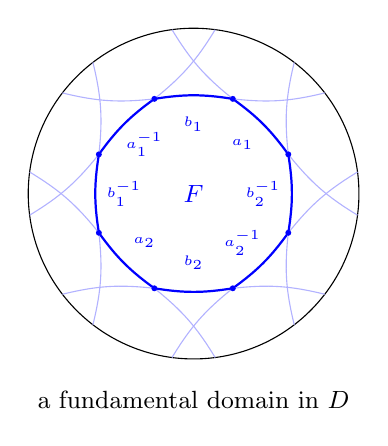
\begin{tikzpicture}[scale=2.1]
	\draw[thin] (0,0) circle (1);
	% vertices of the octagon
	\foreach \i in {0,...,7} { \coordinate (v\i) at ({22.5+45*\i}:0.62); }
	% central octagon; its sides are hyperbolic geodesics, so they bow gently
	% towards the centre
	\foreach \i in {0,...,7} {
		\pgfmathtruncatemacro\j{mod(\i+1,8)}
		\draw[thick, color=blue] (v\i) to[bend right=9] (v\j);
	}
	\node[color=blue] at (0,0) {\small $F$};
	% the geodesics continue out to the boundary, cutting off the neighbouring tiles
	\foreach \i in {0,...,7} {
		\pgfmathsetmacro\a{22.5+45*\i}
		\draw[thin, color=blue!30] (v\i) to[bend right=10] ({\a-30}:1);
		\draw[thin, color=blue!30] (v\i) to[bend left=10] ({\a+30}:1);
	}
	\foreach \i in {0,...,7} { \fill[color=blue] (v\i) circle (0.018); }
	% side identifications, as in the Euclidean octagon above
	\foreach \i/\lab in {0/{a_1}, 1/{b_1}, 2/{a_1^{-1}}, 3/{b_1^{-1}},
		4/{a_2}, 5/{b_2}, 6/{a_2^{-1}}, 7/{b_2^{-1}}} {
		\pgfmathsetmacro\a{45+45*\i}
		\node[color=blue] at (\a:0.42) {\tiny $\lab$};
	}
	\node at (0,-1.25) {\small a fundamental domain in $\disc$};
\end{tikzpicture}
\end{center}

\subsection{Consequences of Uniformisation}

We close with two classical theorems which fall out of the machine.

\begin{theorem}[Riemann Mapping Theorem]
	Every simply connected domain $D \subsetneq \C$ is conformally equivalent to $\disc$.
\end{theorem}

\begin{proof}
	$D$ is a simply connected Riemann surface, so by Theorem \ref{thm:uniformisation} it is
	$\Cinf$, $\C$ or $\disc$. It is not $\Cinf$, being non-compact. Suppose
	$f : \C \to D$ were a conformal equivalence. Composing with the inclusion
	$D \hookrightarrow \C$ gives an injective entire function $f$; by
	Casorati--Weierstrass its singularity at $\infty$ is not essential (an injective
	function cannot take values densely near $\infty$ while being open near a fixed finite
	point), so $f$ extends to a holomorphic $\bar f : \Cinf\to\Cinf$. This is non-constant,
	so it is surjective by Corollary \ref{cor:compactsurjective}; injectivity of $f$ then
	forces $\bar f(\infty)=\infty$ and $D = f(\C) = \C$, contradicting $D \subsetneq\C$.
	So $D\cong\disc$.
\end{proof}

It is worth noticing how the logic runs: uniformisation is the general theorem and the
Riemann mapping theorem is a special case, whereas historically the implication is
usually run the other way (the Riemann mapping theorem being an ingredient in proofs of
uniformisation).

\begin{theorem}[Little Picard Theorem]
	Every holomorphic function $f : \C \to \C\setminus\{0,1\}$ is constant.
\end{theorem}

\begin{proof}
	The surface $\C\setminus\{0,1\}$ is uniformised by $\disc$: it is not $\Cinf$ or $\C$
	or $\Cs$ or a torus, so by Propositions \ref{prop:uniformbyCinf} and
	\ref{prop:uniformbyC} its universal cover is $\disc$. (One can also exhibit the covering
	explicitly using the modular $\lambda$-function; this is on the example sheets.)

	Let $\pi : \disc \to \C\setminus\{0,1\}$ be the uniformising map. As $\C$ is simply
	connected, Lemma \ref{lem:lifting} gives a holomorphic $F : \C \to \disc$ with
	$f = \pi\circ F$. But $F$ is a bounded entire function, hence constant by Liouville, so
	$f$ is constant.
\end{proof}

Of course $\{0,1\}$ may be replaced by any two distinct points of $\C$, by composing with
a suitable affine map. The theorem is a dramatic strengthening of Liouville: an entire
function which omits merely \emph{two} values is constant. That such a statement should
follow from a covering-space argument -- with no estimate in sight -- is a fair summary of
what Riemann surfaces are for.

\end{document}
